
%%%
%%%
%%%

\section{Kinematic distributions}
\label{sec:results_kinematic_distributions}
The realistic NUHM2 model and the simplified Higgsino model are similar except the $m_{\widetilde{\chi}^{\pm}_{1}}$ is not exactly half way between $m_{\widetilde{\chi}^{0}_{2}}$ and $m_{\widetilde{\chi}^{0}_{1}}$.
The ratio between the $\Delta m(\widetilde{\chi}^{0}_{2}, \widetilde{\chi}^{0}_{1})$ and $\Delta m(\widetilde{\chi}^{\pm}_{1}, \widetilde{\chi}^{0}_{1})$ varies from 1.61 to 1.21 as shown in Table~\ref{tab:data_mass_splitting_ratio}.
The sensitivity of the NUHM2 model used for the 2$\ell$ final state Higgsino analysis is examined by comparing the kinematic distributions of the NUHM2 signal samples and the simplied Higgsino model grid mass points.

All kinematic distributions in the trutl level are very similar and the largest difference is in the $m_{\ell \ell}$ distribution due to the mass splitings $\Delta m(\widetilde{\chi}^{0}_{2}, \widetilde{\chi}^{0}_{1})$ and $\Delta m(\widetilde{\chi}^{\pm}_{1}, \widetilde{\chi}^{0}_{1})$.
This distinguish feature motivates the NUHM2 interpretation.

\begin{figure}[htbp]
    \begin{center}
        \begin{subfigure}[b]{0.48\textwidth}
            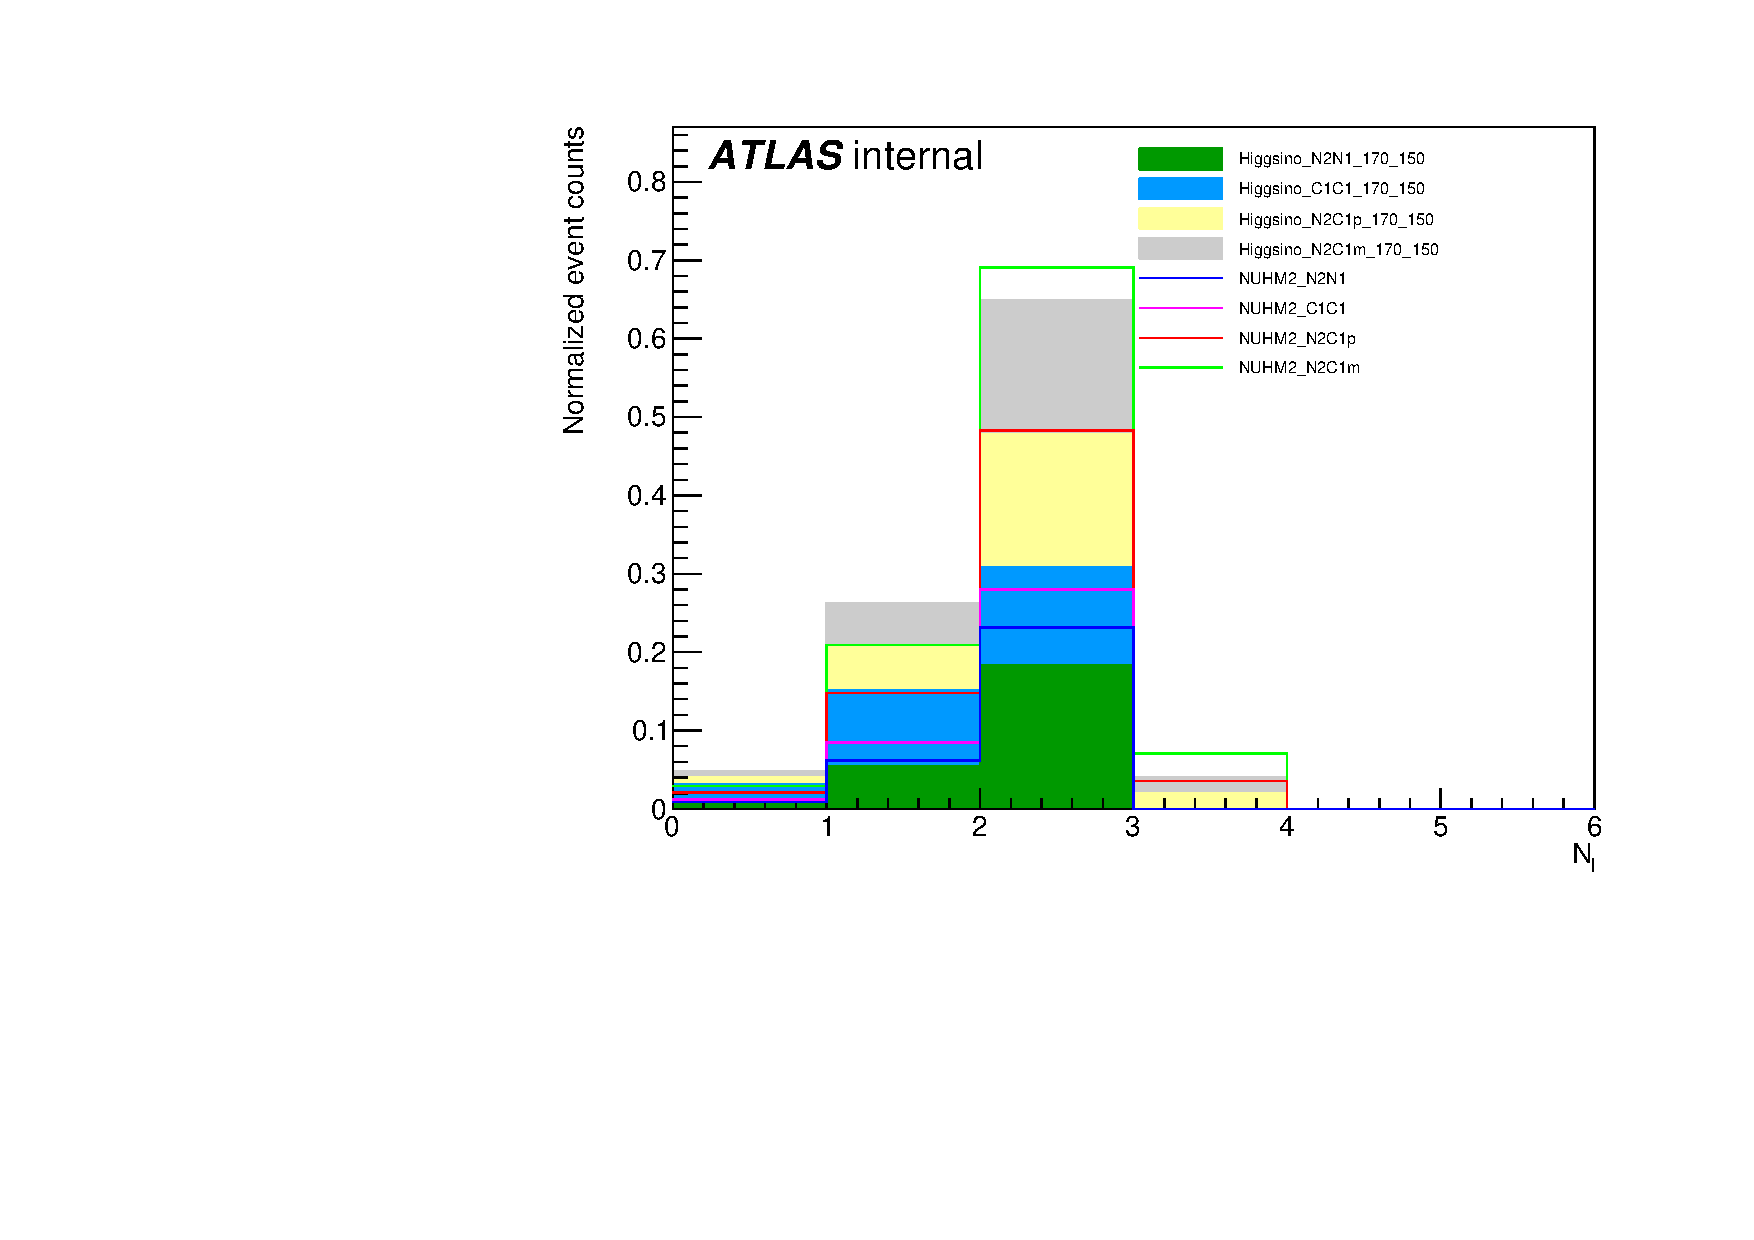
\includegraphics[scale=0.4]{nBaselineLeptons.pdf}
            \caption{Baseline leptons multiplicities}
        \end{subfigure}
        \begin{subfigure}[b]{0.48\textwidth}
            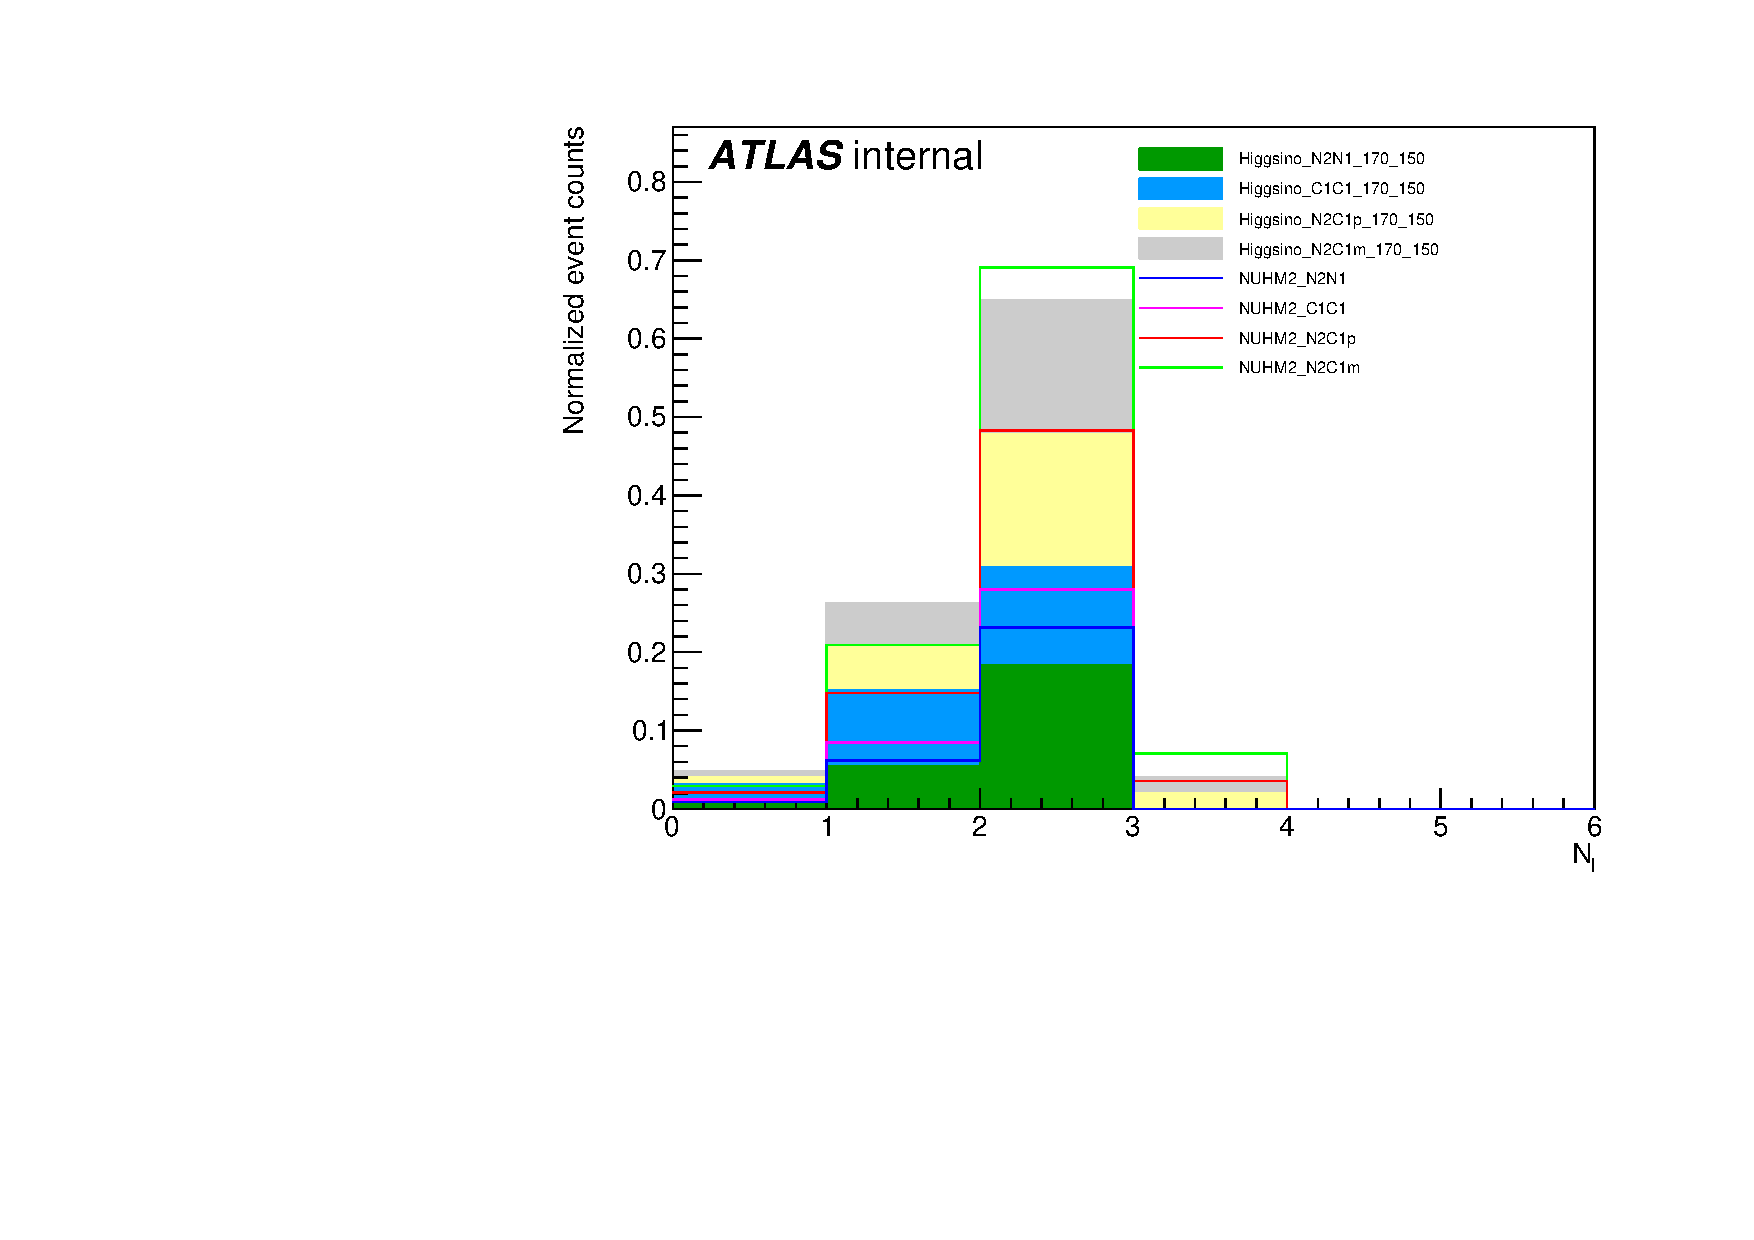
\includegraphics[scale=0.4]{nSignalLeptons.pdf}
            \caption{Signal leptons multiplicities}
        \end{subfigure}
        \begin{subfigure}[b]{0.48\textwidth}
            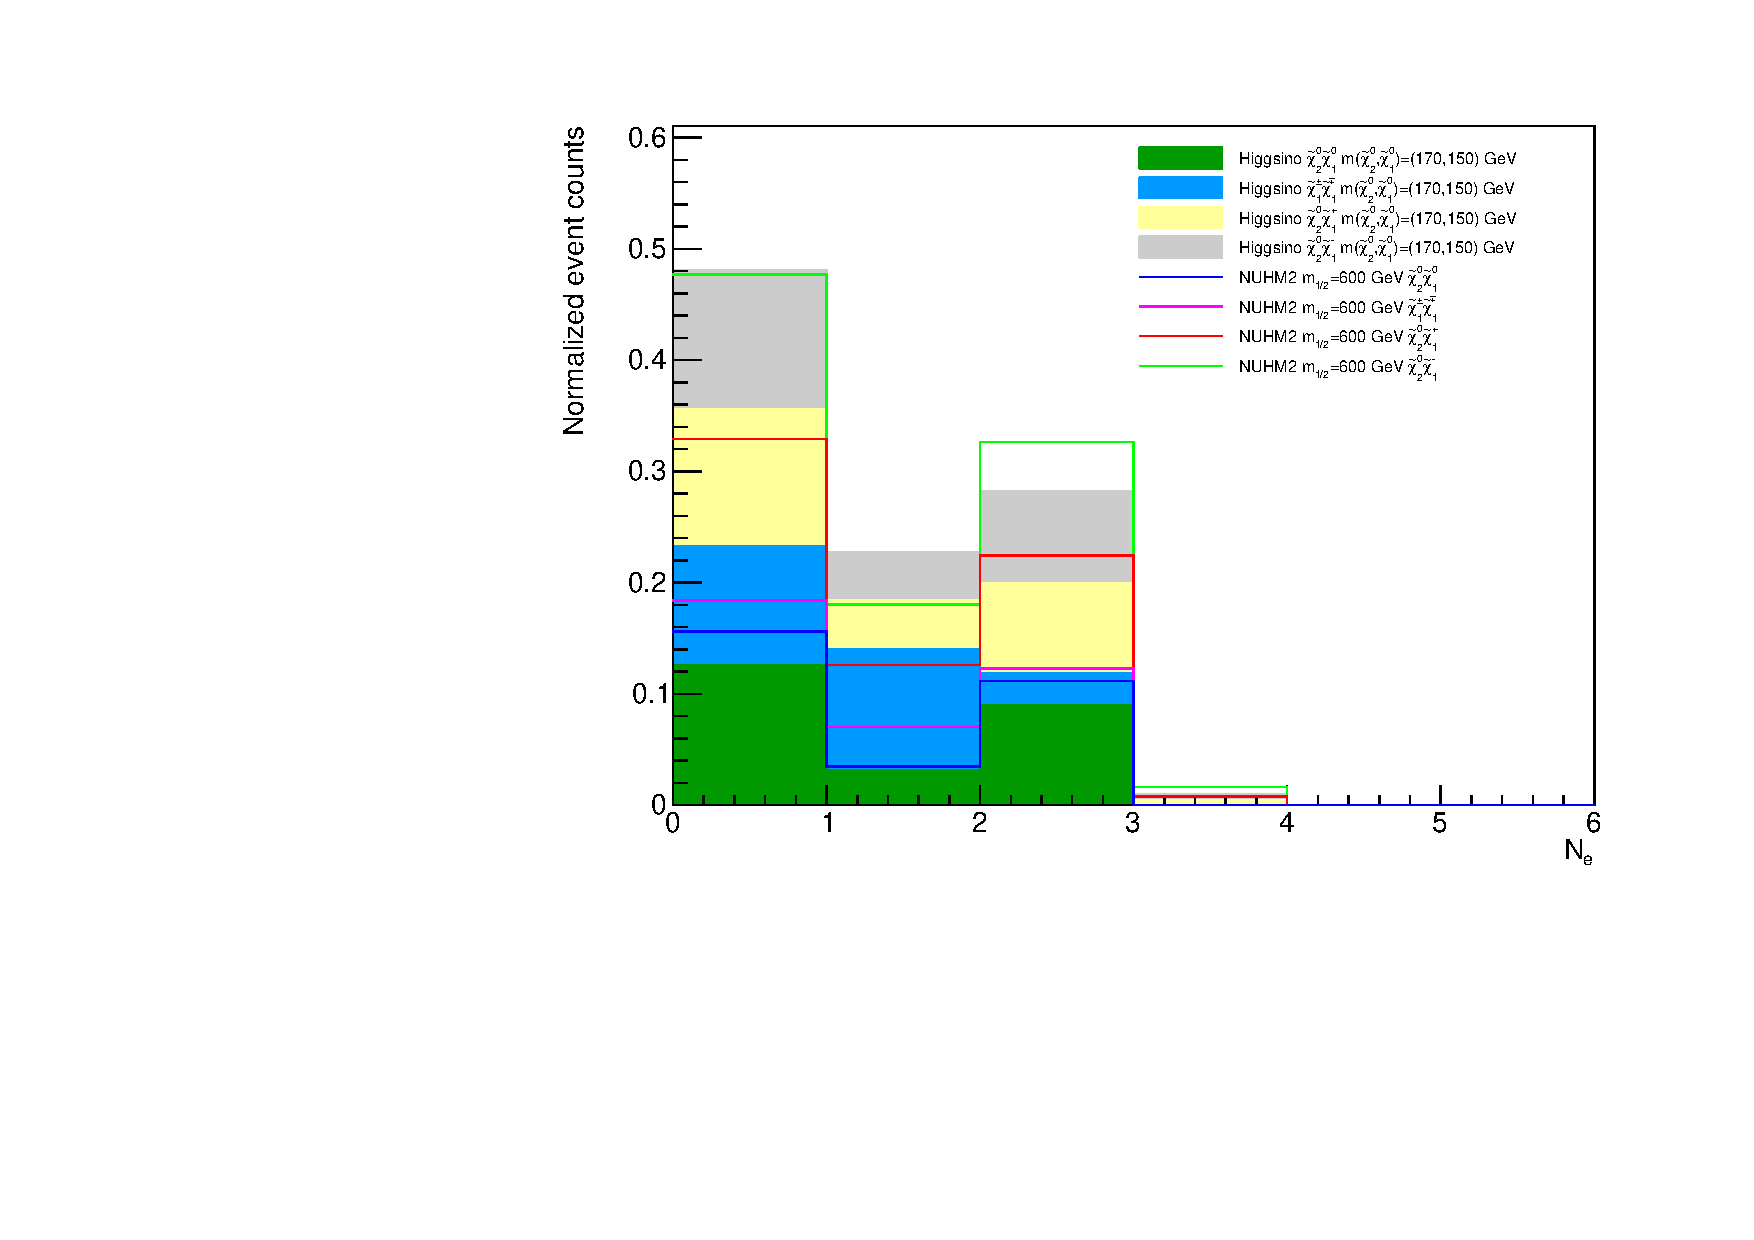
\includegraphics[scale=0.4]{nElectrons.pdf}
            \caption{Signal electrons multiplicities}
        \end{subfigure}
        \begin{subfigure}[b]{0.48\textwidth}
            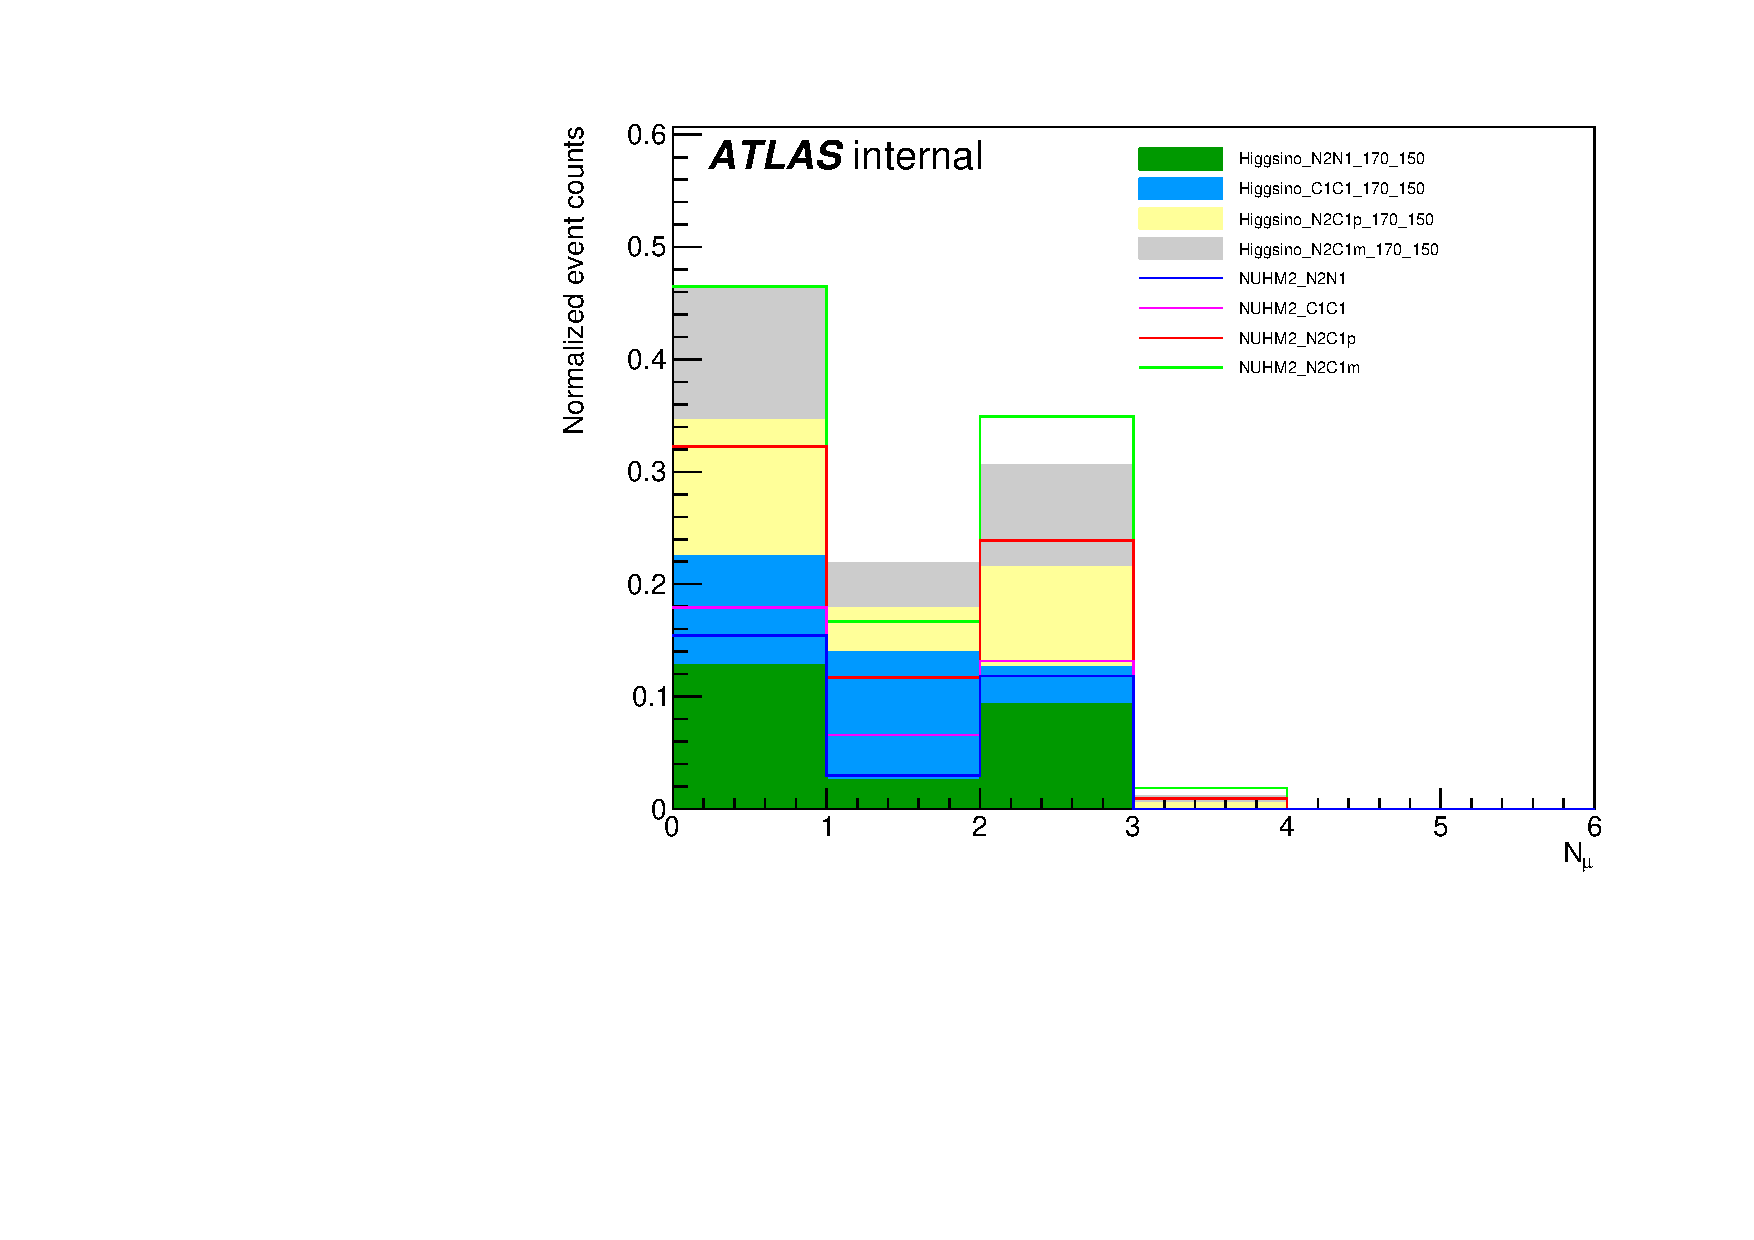
\includegraphics[scale=0.4]{nMuons.pdf}
            \caption{Signal muons multiplicities}
        \end{subfigure}
    \end{center}
    \caption{The lepton multiplicity distributions.
    The lepton multiplicity of NUHM2 with $m_{1/2} = 600$~{\GeV} are compared to the simplified Higgsino model with $m_{\widetilde{\chi}^{0}_{2}}=170$~{\GeV} and $m_{\widetilde{\chi}^{0}_{1}}=150$~{\GeV}.
    Four different production channels, $\widetilde{\chi}^{0}_{2}\widetilde{\chi}^{0}_{1}$, $\widetilde{\chi}^{0}_{2}\widetilde{\chi}^{+}_{1}$, $\widetilde{\chi}^{0}_{2}\widetilde{\chi}^{-}_{1}$, and $\widetilde{\chi}^{\pm}_{1}\widetilde{\chi}^{\mp}_{1}$, for the NUHM2 and the simplified Higgsino model are considered.
    The distributions of four productions are combined and normalized to equal area.}
    \label{fig:results_nuhm2_lepton_multiplicity}
\end{figure}

\begin{figure}[htbp]
    \begin{center}
        \begin{subfigure}[b]{0.48\textwidth}
            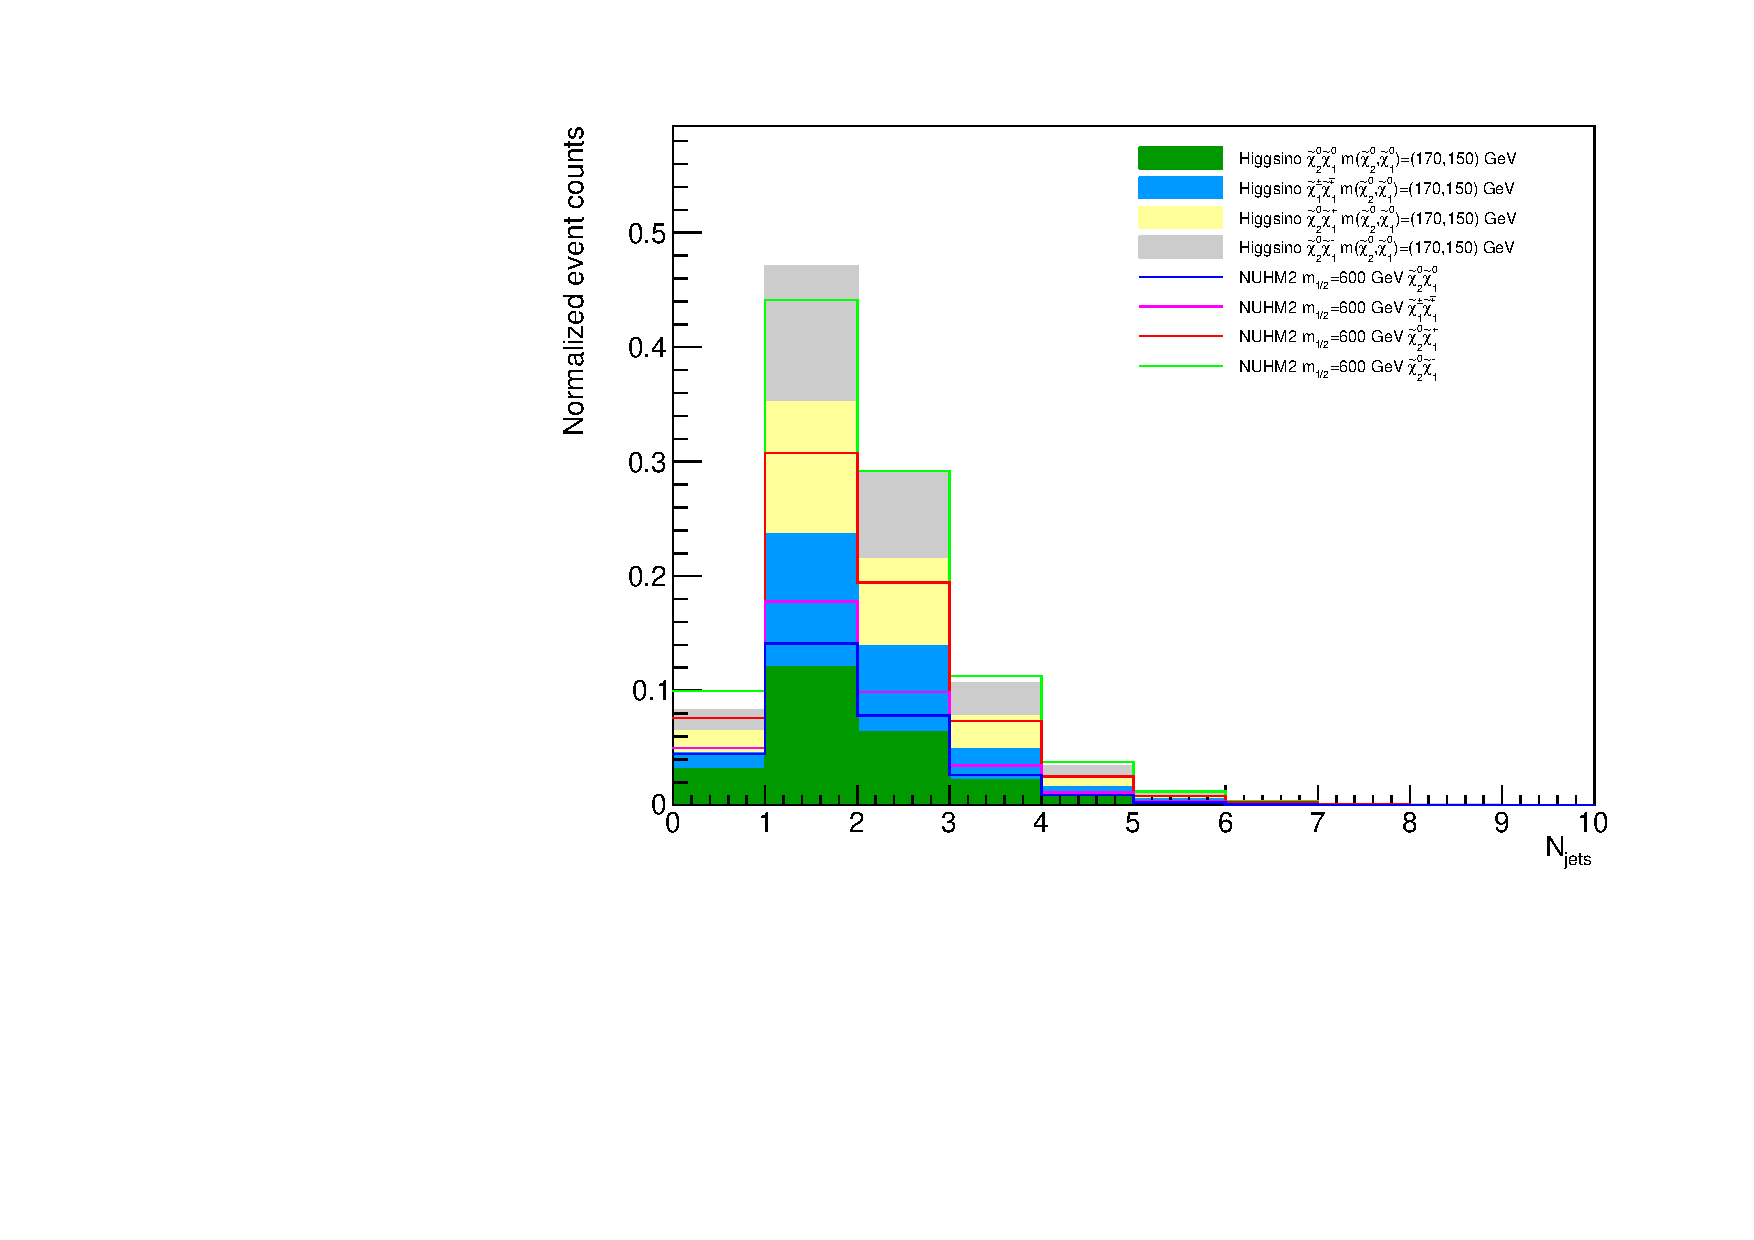
\includegraphics[scale=0.4]{nJets.pdf}
            \caption{Jets multiplicity}
        \end{subfigure}
        \begin{subfigure}[b]{0.48\textwidth}
            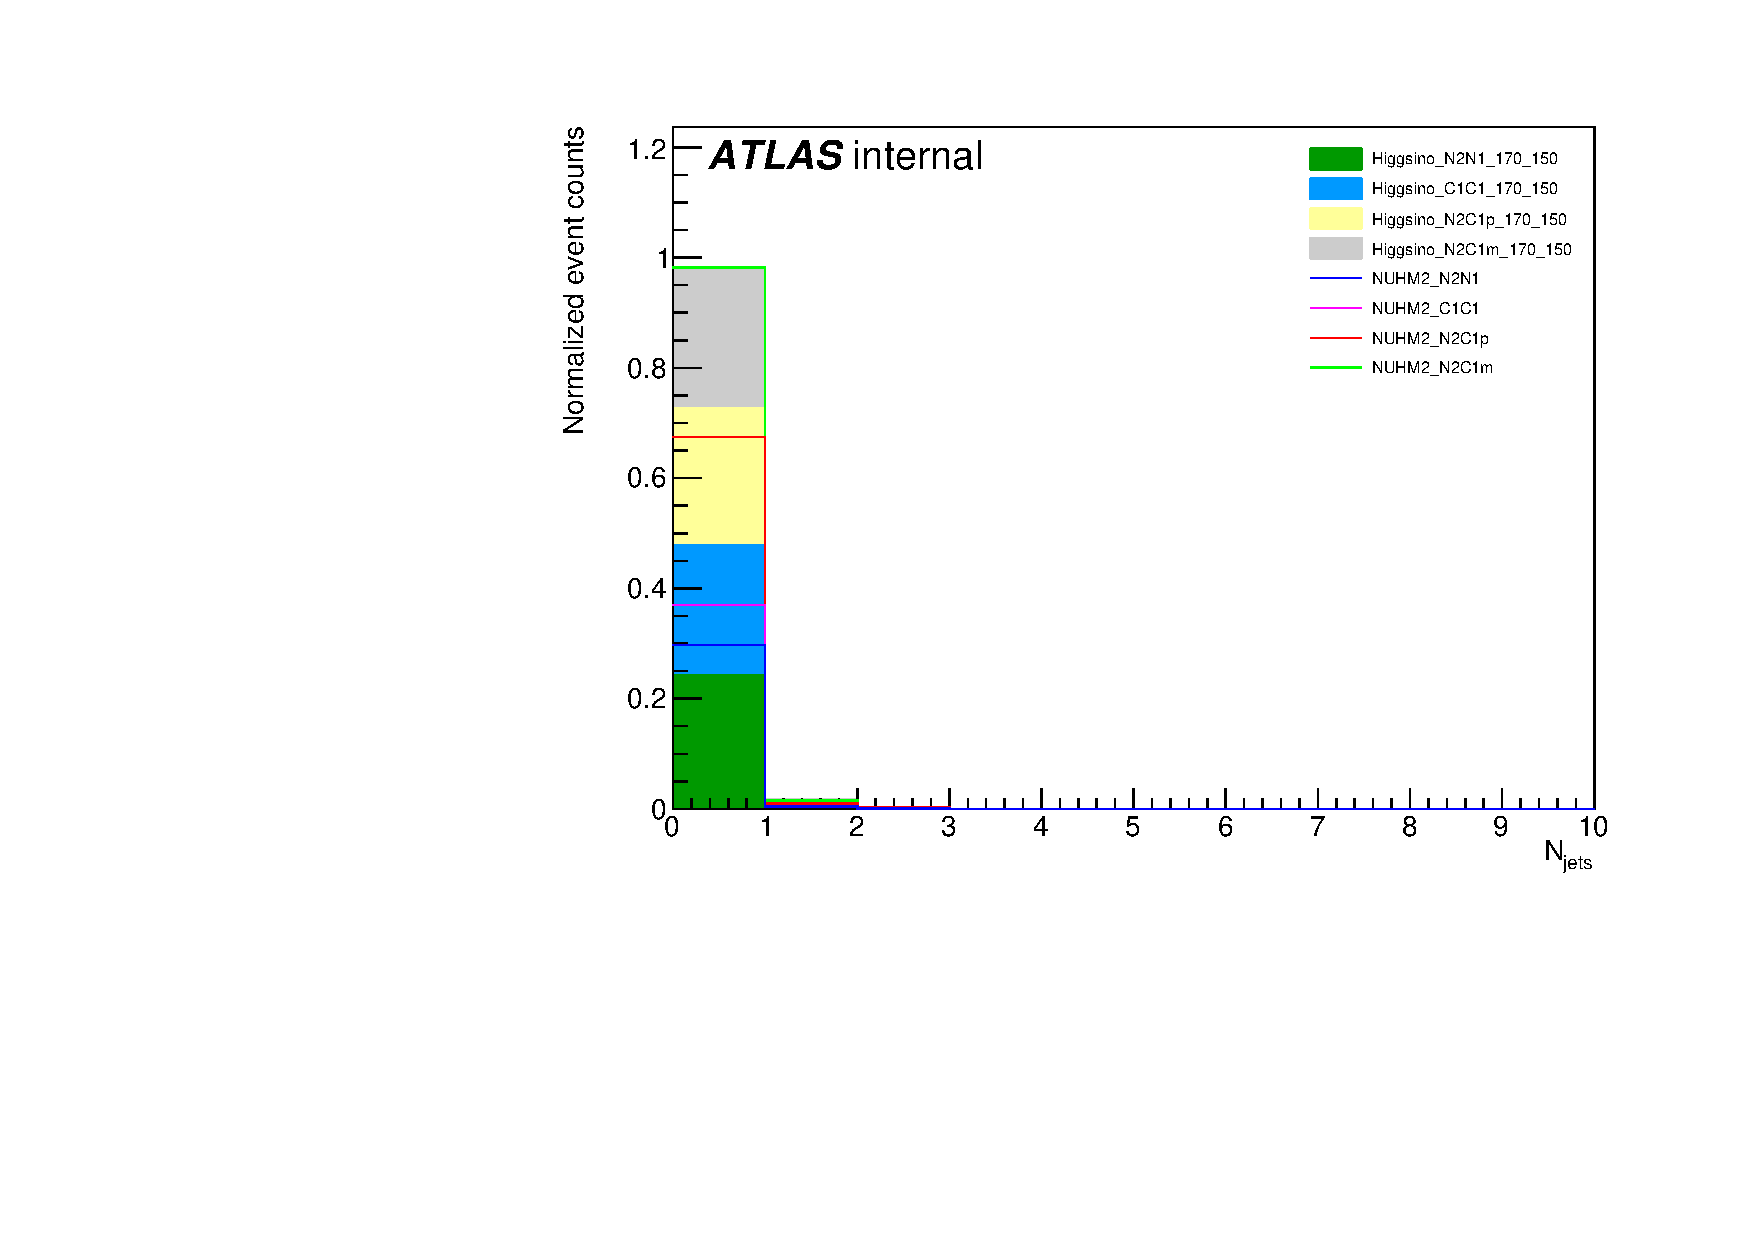
\includegraphics[scale=0.4]{nBjets.pdf}
            \caption{$b$-jets multiplicity}
        \end{subfigure}
        \begin{subfigure}[b]{0.48\textwidth}
            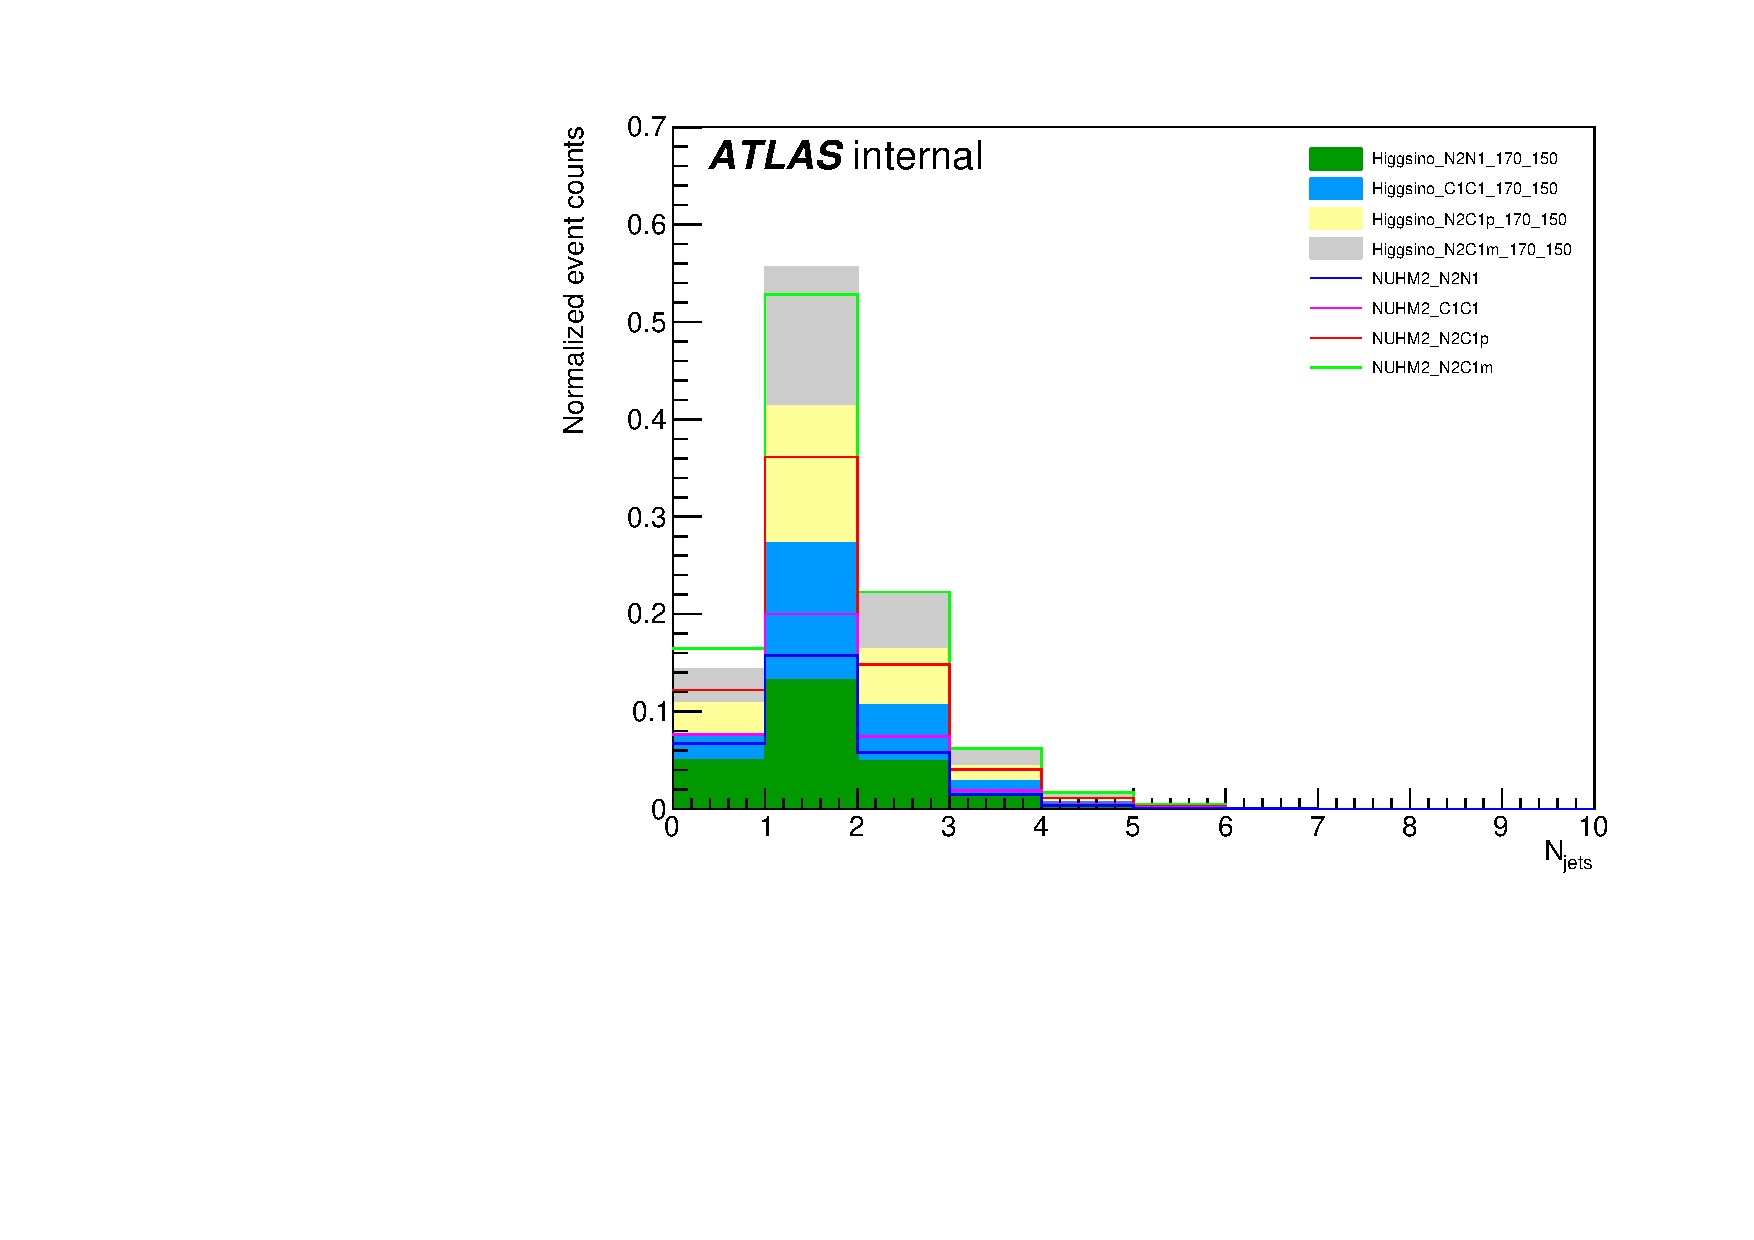
\includegraphics[scale=0.4]{nJet25.pdf}
            \caption{Signal jets multiplicity with $\pt > 25$~{\GeV}}
        \end{subfigure}
        \begin{subfigure}[b]{0.48\textwidth}
            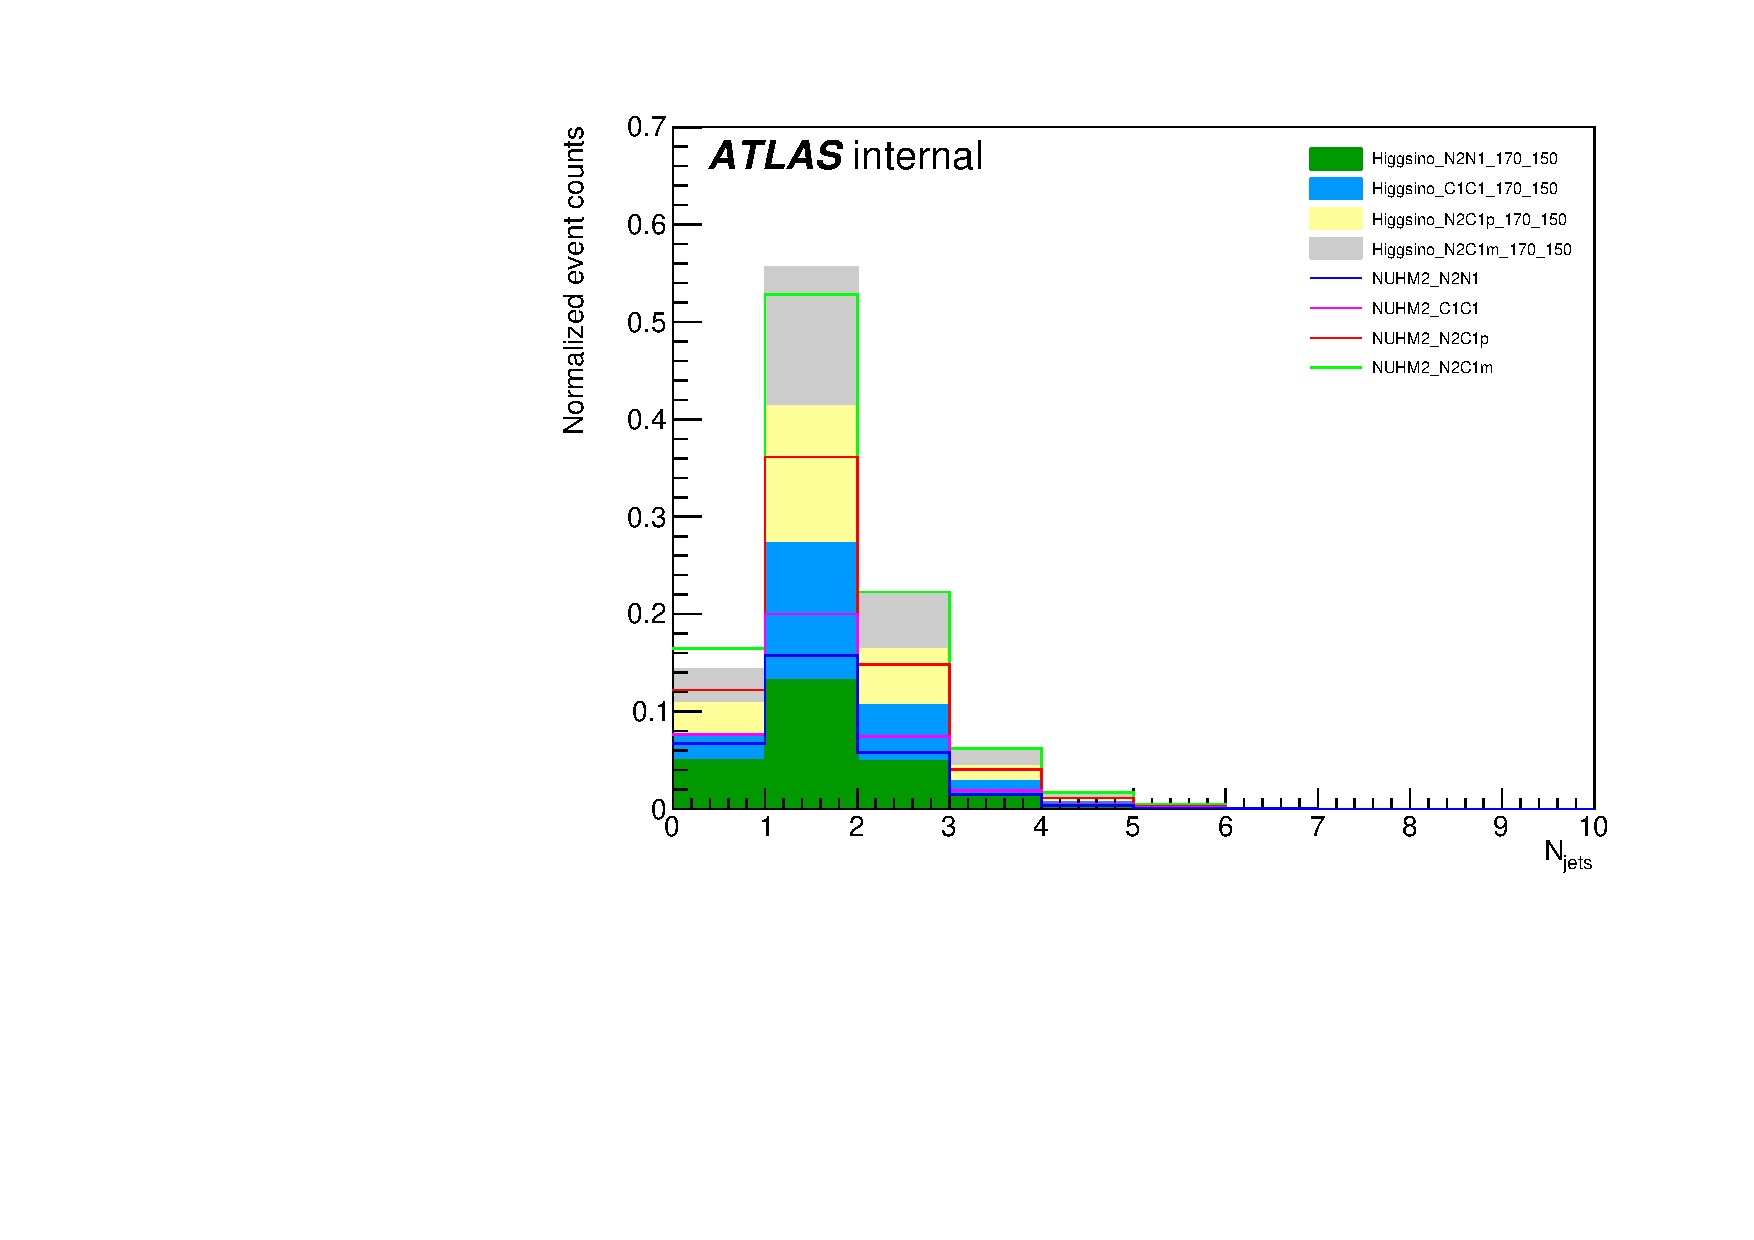
\includegraphics[scale=0.4]{nJet30.pdf}
            \caption{Signal jets multiplicity with $\pt > 30$~{\GeV}}
        \end{subfigure}
    \end{center}
    \caption{The jets multiplicity distributions.
    The jet multiplicity of NUHM2 with $m_{1/2} = 600$~{\GeV} are compared to the simplified Higgsino model with $m_{\widetilde{\chi}^{0}_{2}}=170$~{\GeV} and $m_{\widetilde{\chi}^{0}_{1}}=150$~{\GeV}.
    The top left plot includes the forward jets and the bottom two plots use the signal jets with $\pt > 25$~{\GeV} and $\pt > 30$~{\GeV}, respectively.
    Four different production channels, $\widetilde{\chi}^{0}_{2}\widetilde{\chi}^{0}_{1}$, $\widetilde{\chi}^{0}_{2}\widetilde{\chi}^{+}_{1}$, $\widetilde{\chi}^{0}_{2}\widetilde{\chi}^{-}_{1}$, and $\widetilde{\chi}^{\pm}_{1}\widetilde{\chi}^{\mp}_{1}$, for the NUHM2 and the simplified Higgsino model are considered.
    The distributions of four productions are combined and normalized to equal area.}
    \label{fig:results_nuhm2_jets_multiplicity}
\end{figure}

\begin{figure}[htbp]
    \begin{center}
        \begin{subfigure}[b]{0.48\textwidth}
            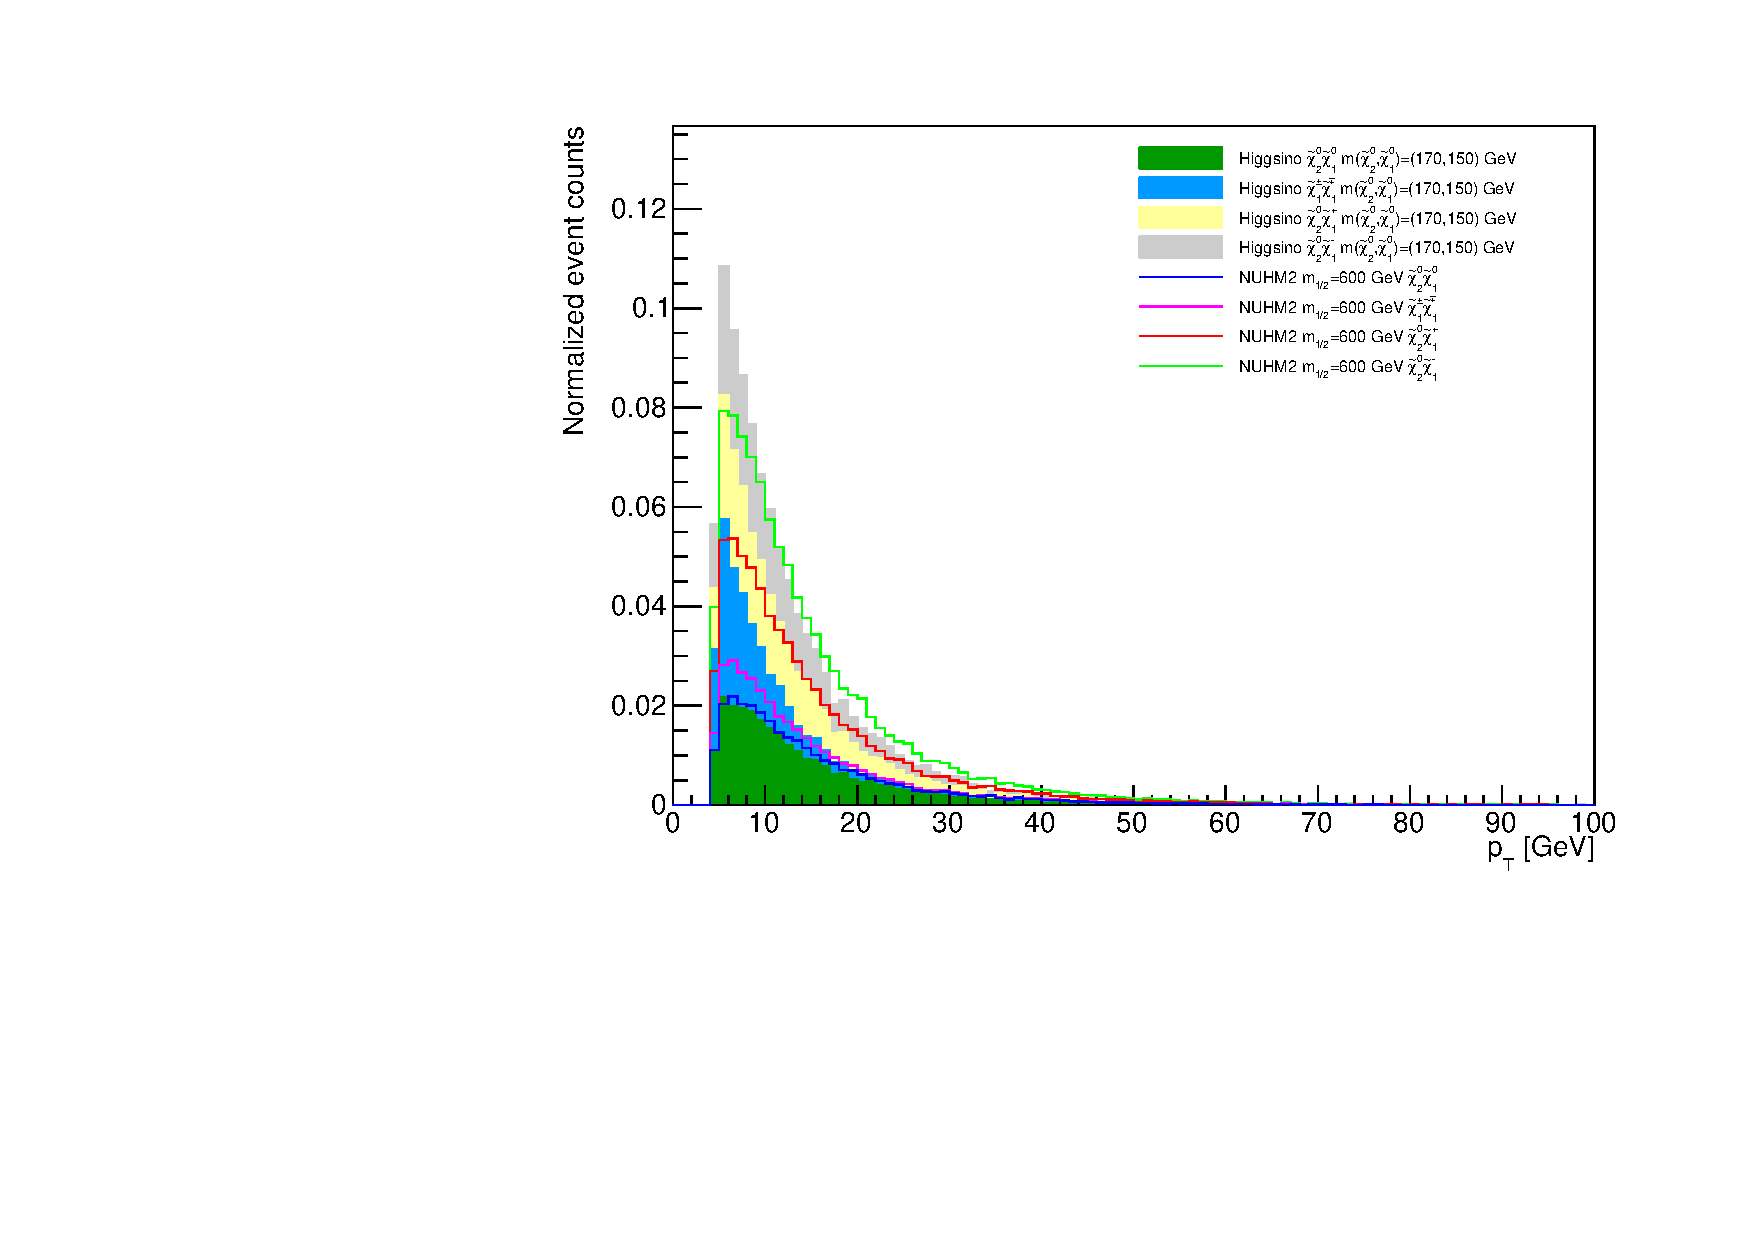
\includegraphics[scale=0.35]{signalElectrons_pt.pdf}
            \caption{Signal electrons \pt}
        \end{subfigure}
        \begin{subfigure}[b]{0.48\textwidth}
            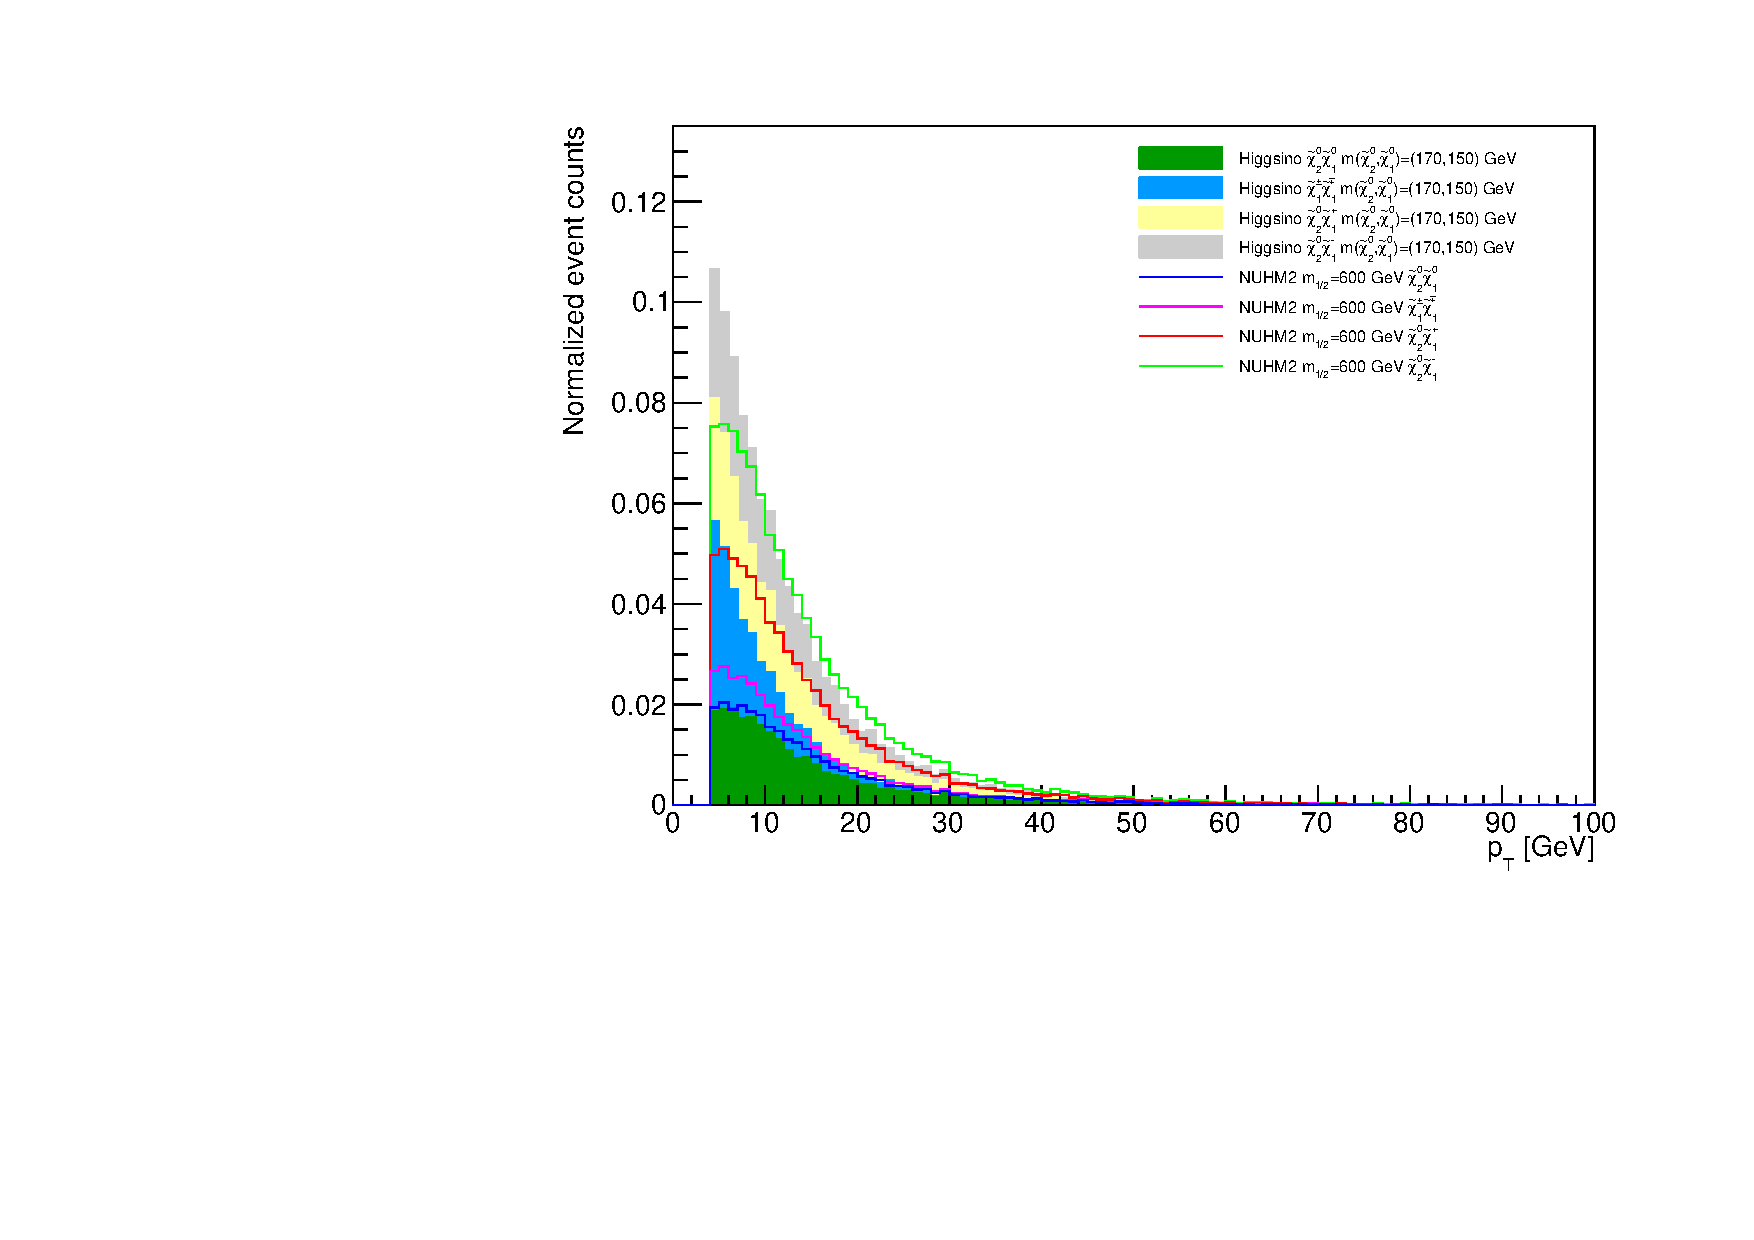
\includegraphics[scale=0.35]{signalMuons_pt.pdf}
            \caption{Signal muons \pt}
        \end{subfigure}
        \begin{subfigure}[b]{0.48\textwidth}
            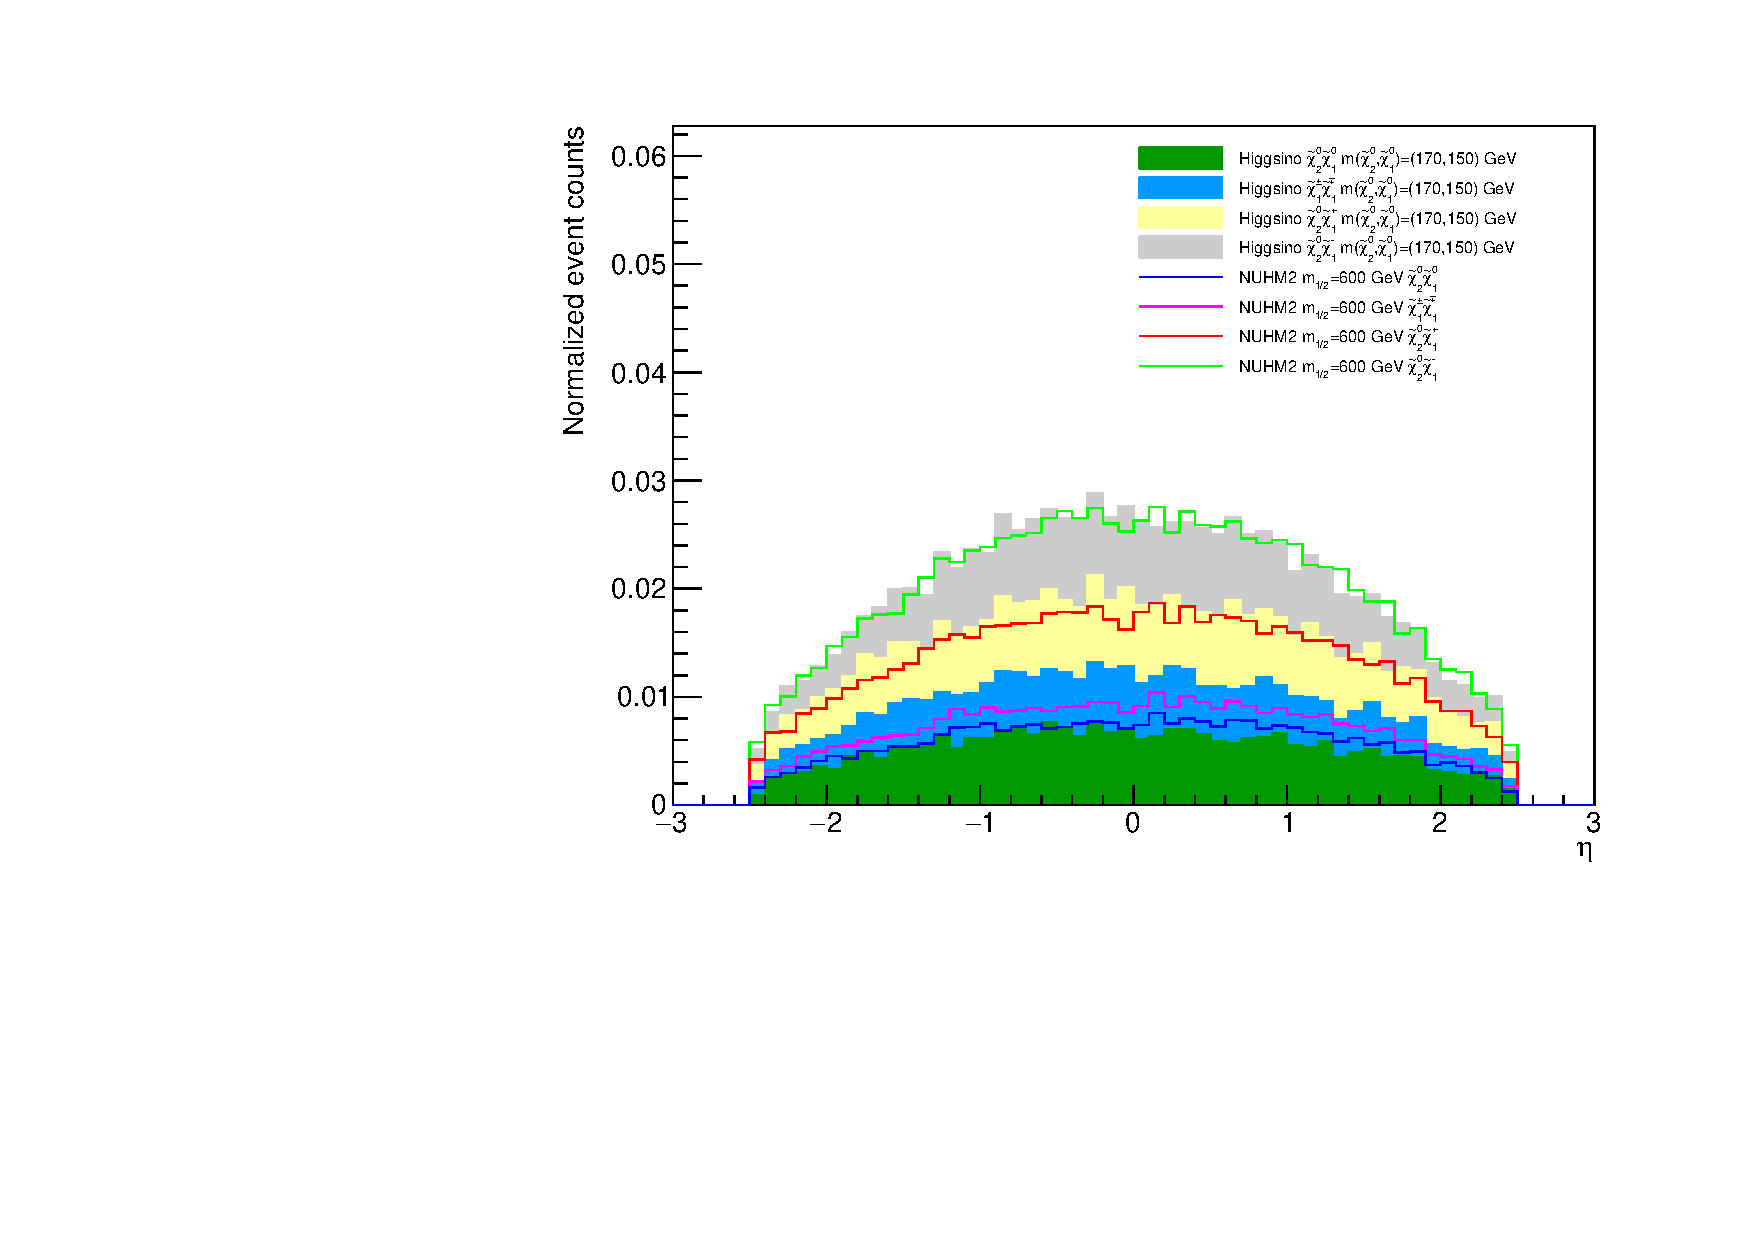
\includegraphics[scale=0.35]{signalElectrons_eta.pdf}
            \caption{Signal electrons $\eta$}
        \end{subfigure}
        \begin{subfigure}[b]{0.48\textwidth}
            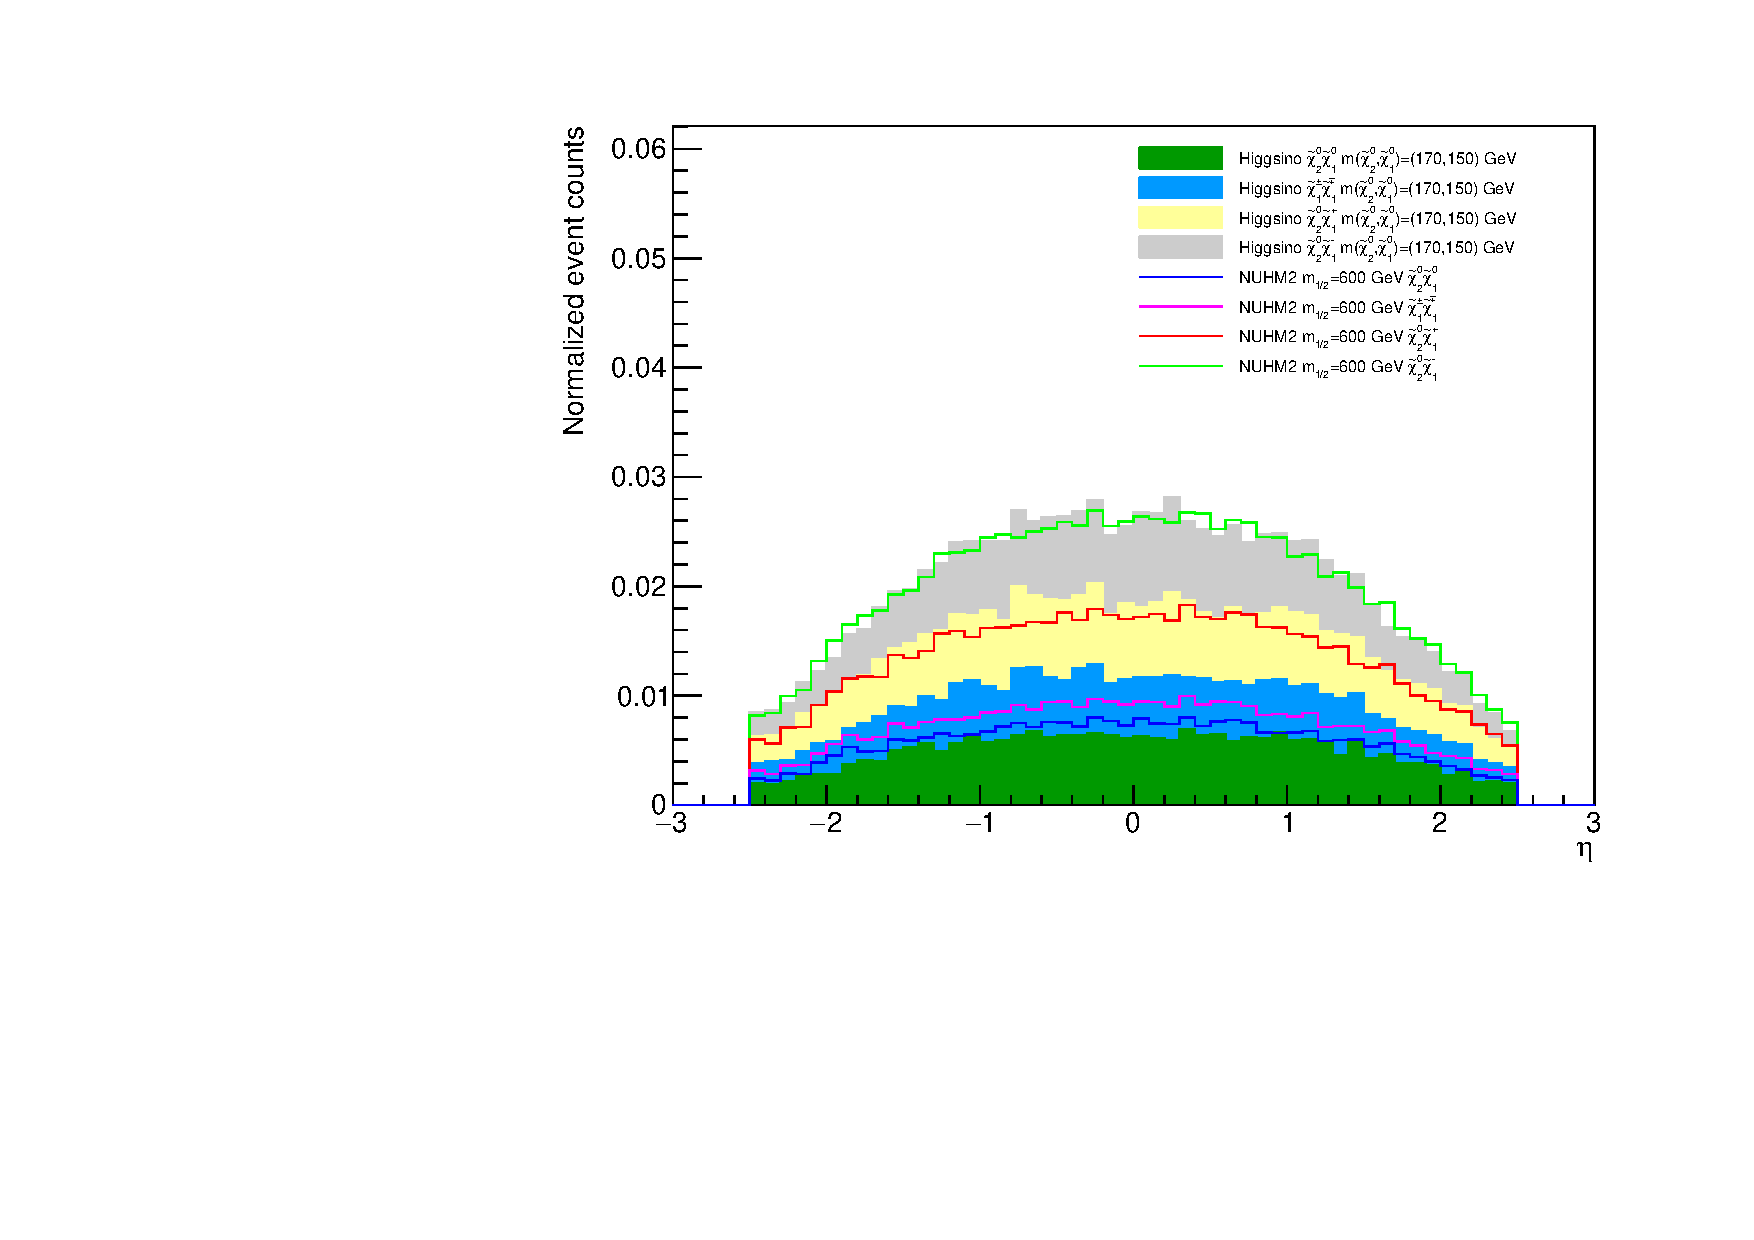
\includegraphics[scale=0.35]{signalMuons_eta.pdf}
            \caption{Signal muons $\eta$}
        \end{subfigure}
        \begin{subfigure}[b]{0.48\textwidth}
            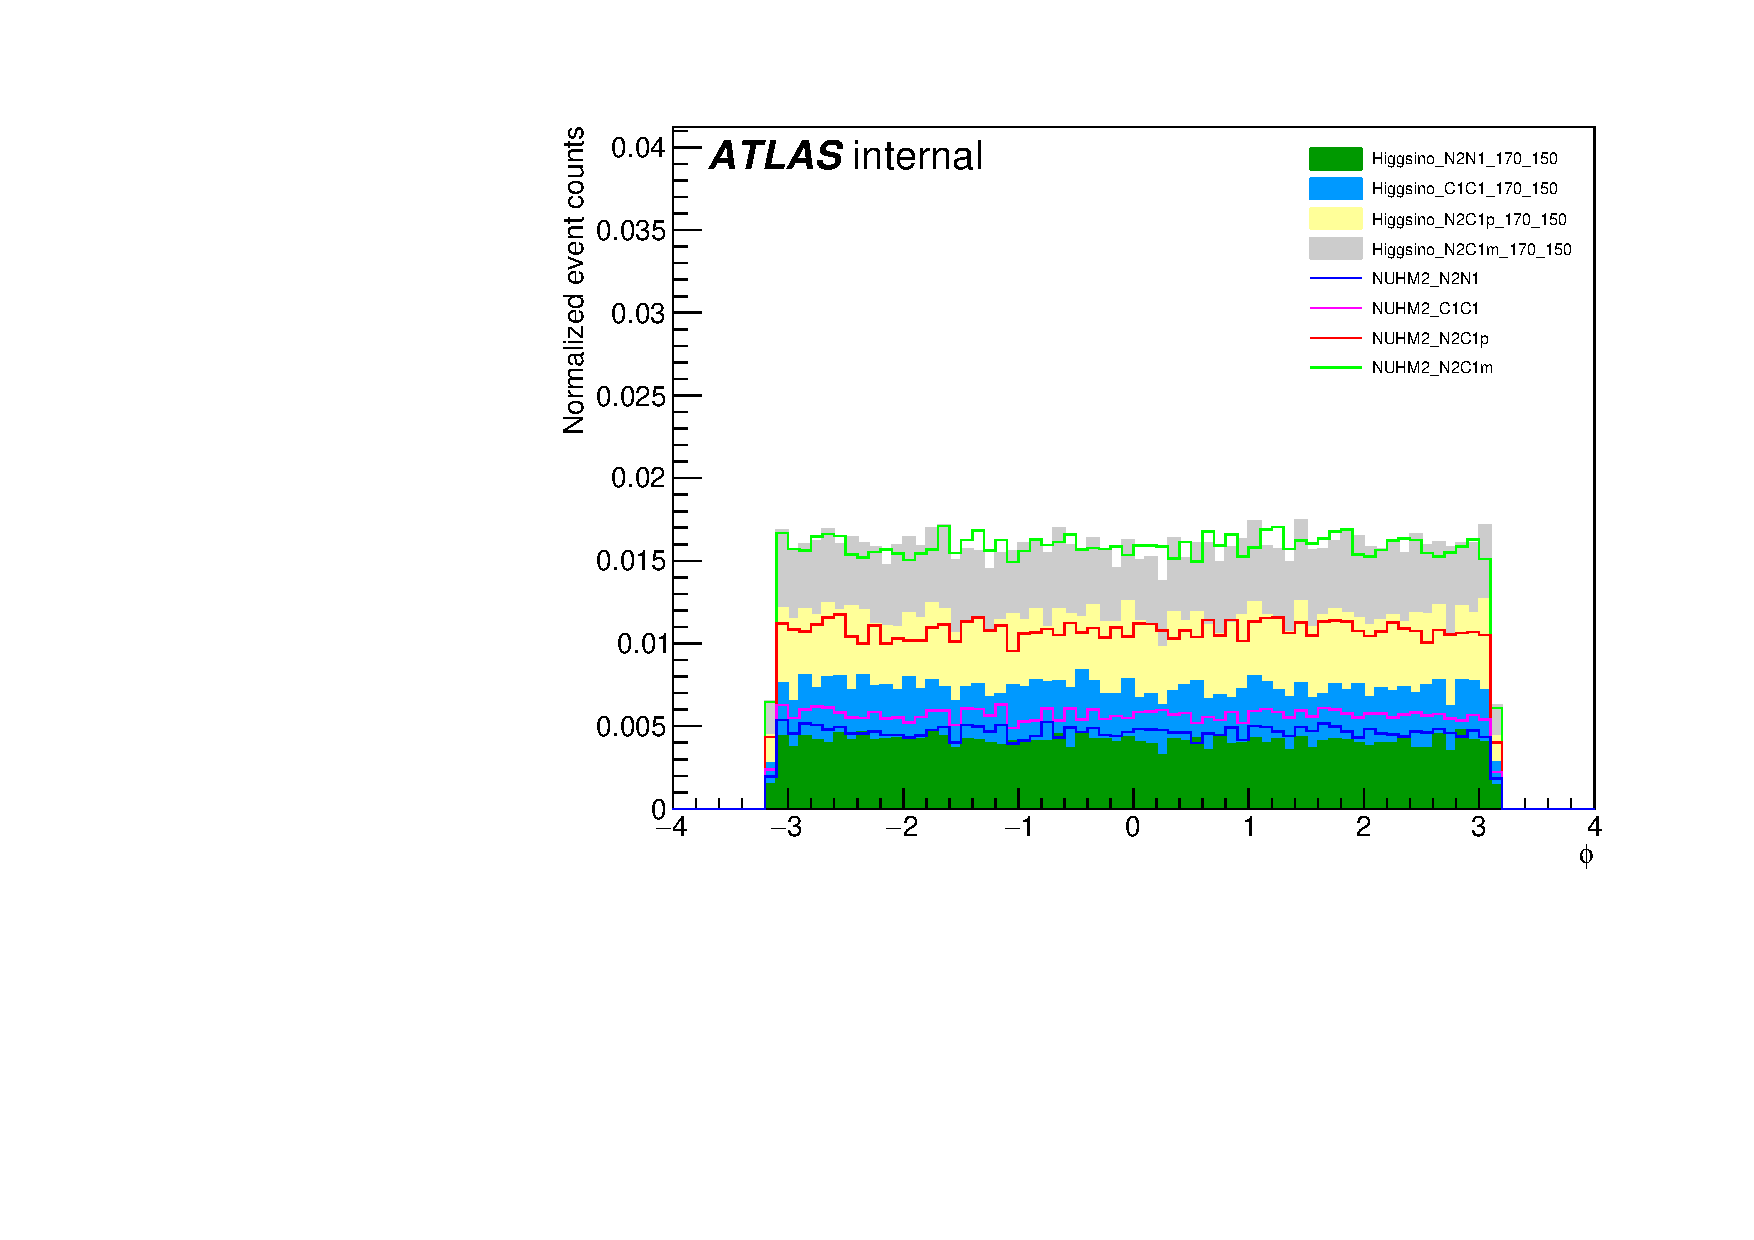
\includegraphics[scale=0.35]{signalElectrons_phi.pdf}
            \caption{Signal electrons $\phi$}
        \end{subfigure}
        \begin{subfigure}[b]{0.48\textwidth}
            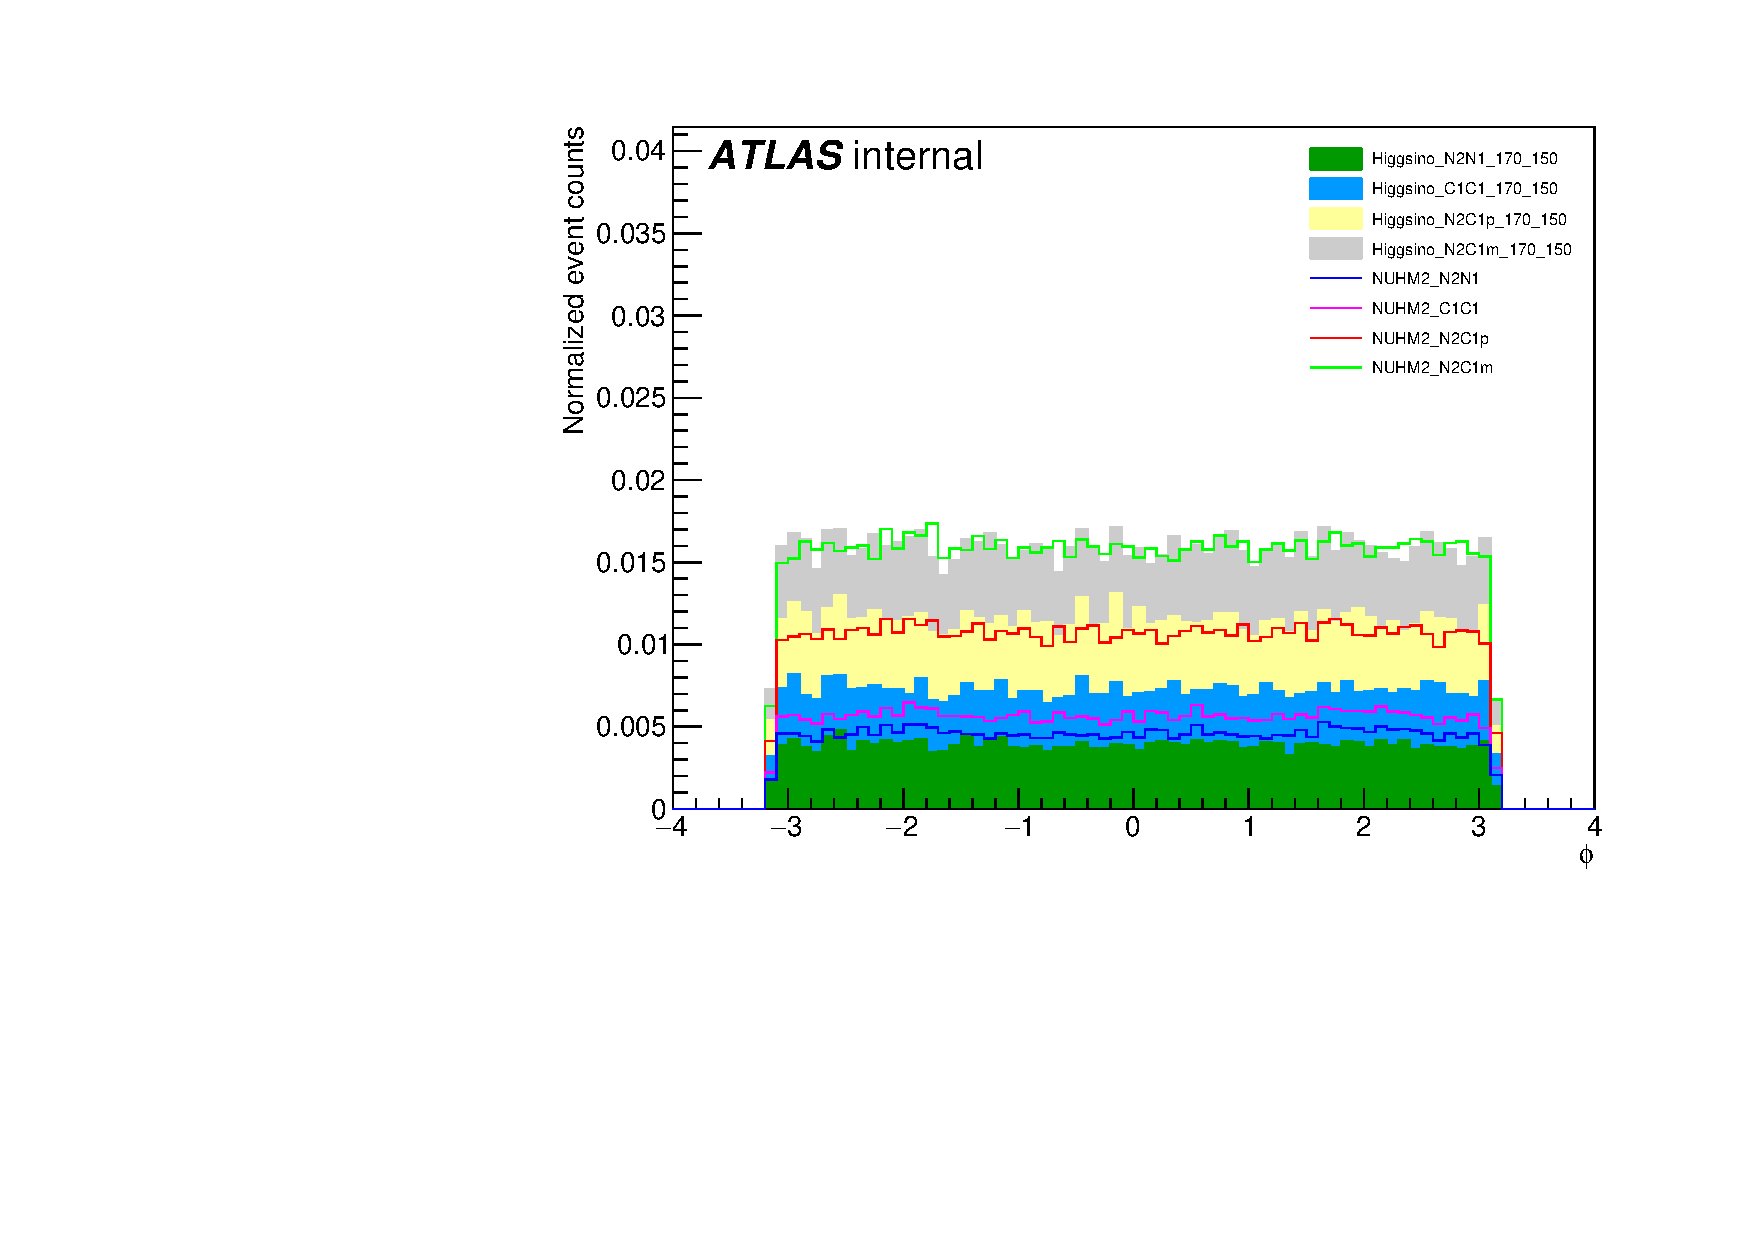
\includegraphics[scale=0.35]{signalMuons_phi.pdf}
            \caption{Signal muons $\phi$}
        \end{subfigure}
    \end{center}
    \caption{The \pt, $\eta$, and $\phi$ distributions for the NUHM2 with $m_{1/2} = 600$~{\GeV} and the simplified Higgsino model with $m_{\widetilde{\chi}^{0}_{2}}=170$~{\GeV} and $m_{\widetilde{\chi}^{0}_{1}}=150$~{\GeV}.
    The signal electrons \pt, $\eta$, and $\phi$ distributions are on the left column and the signal muons distributions are on the right.
    Four different production channels, $\widetilde{\chi}^{0}_{2}\widetilde{\chi}^{0}_{1}$, $\widetilde{\chi}^{0}_{2}\widetilde{\chi}^{+}_{1}$, $\widetilde{\chi}^{0}_{2}\widetilde{\chi}^{-}_{1}$, and $\widetilde{\chi}^{\pm}_{1}\widetilde{\chi}^{\mp}_{1}$, for the NUHM2 and the simplified Higgsino model are considered.
    The distributions of four productions are combined and normalized to equal area.}
    \label{fig:results_nuhm2_leptons_pt_eta_phi}
\end{figure}

\begin{figure}[htbp]
    \begin{center}
        \begin{subfigure}[b]{0.48\textwidth}
            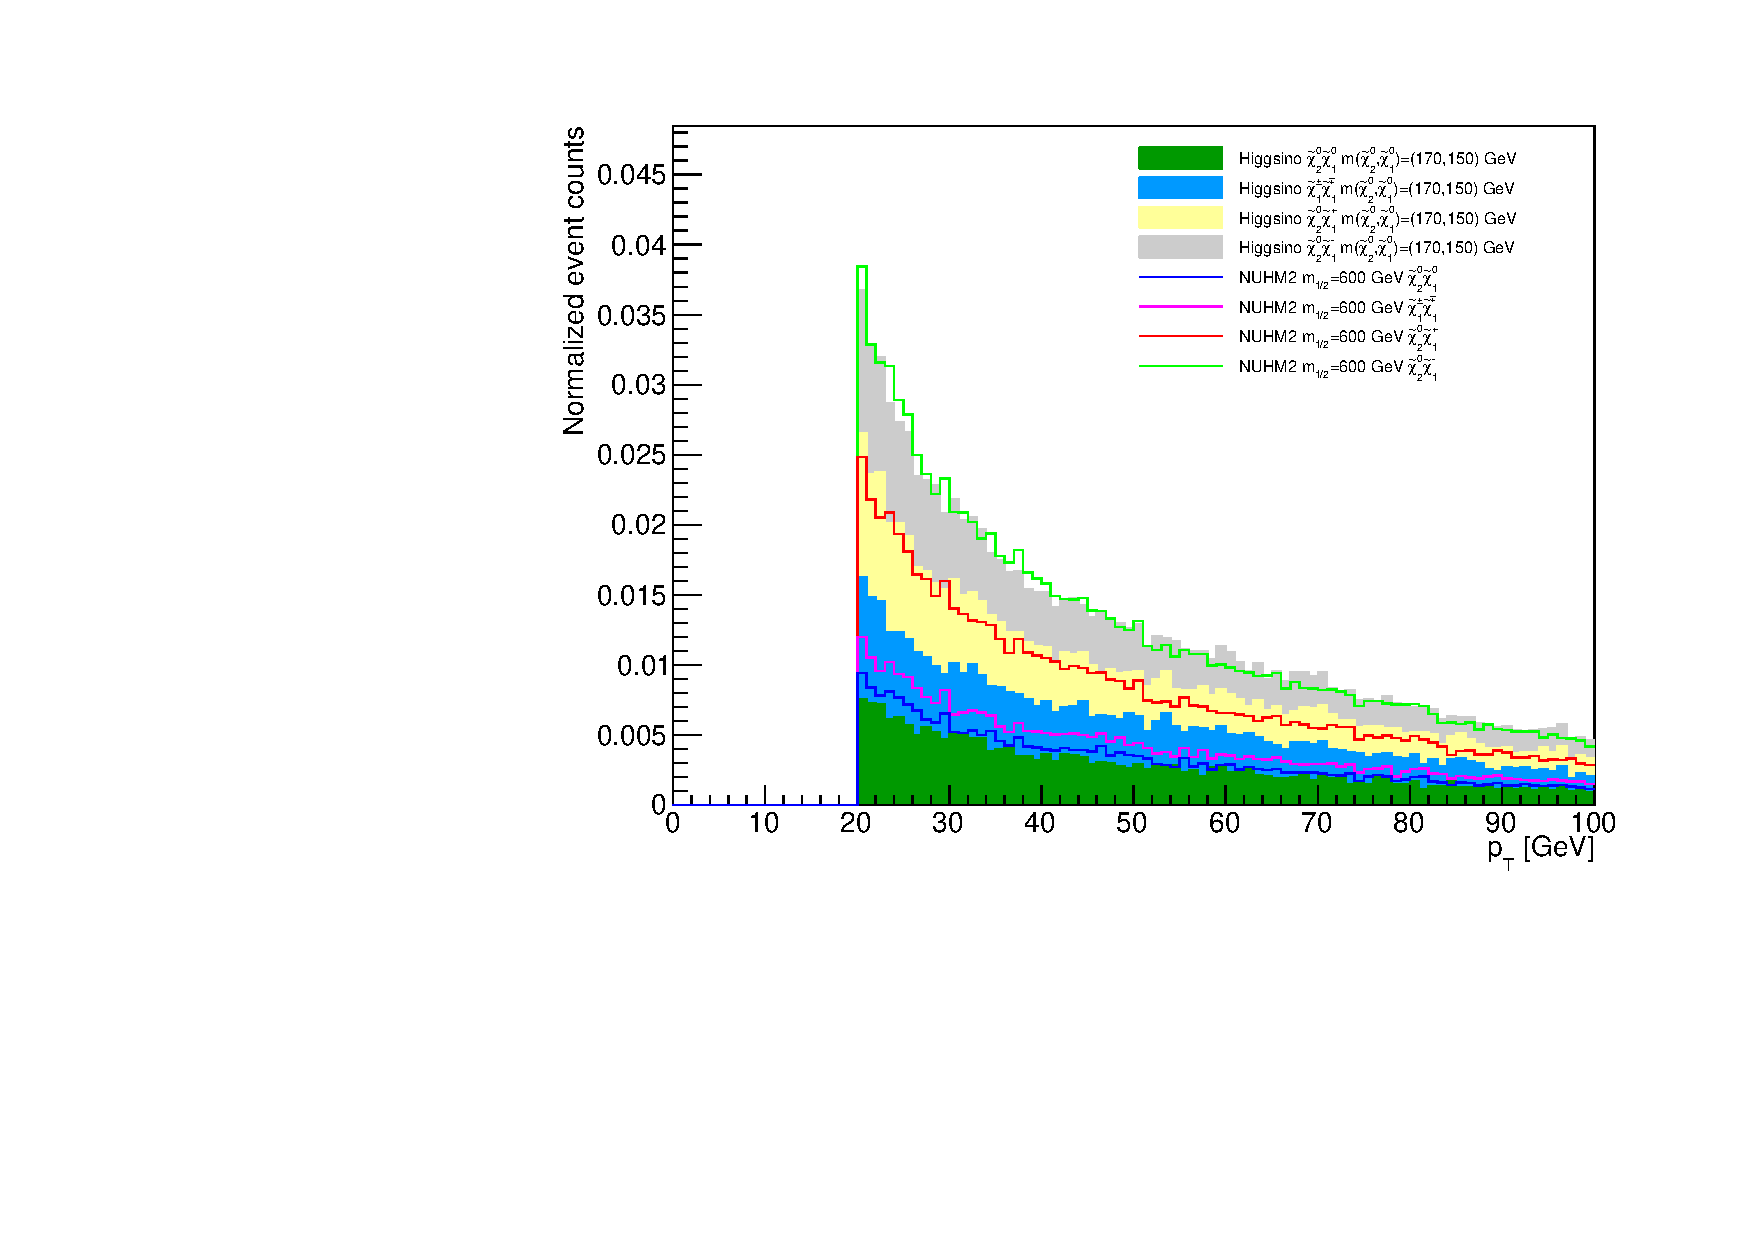
\includegraphics[scale=0.35]{signalJets_pt.pdf}
            \caption{The signal jets \pt.}
        \end{subfigure}
        \begin{subfigure}[b]{0.48\textwidth}
            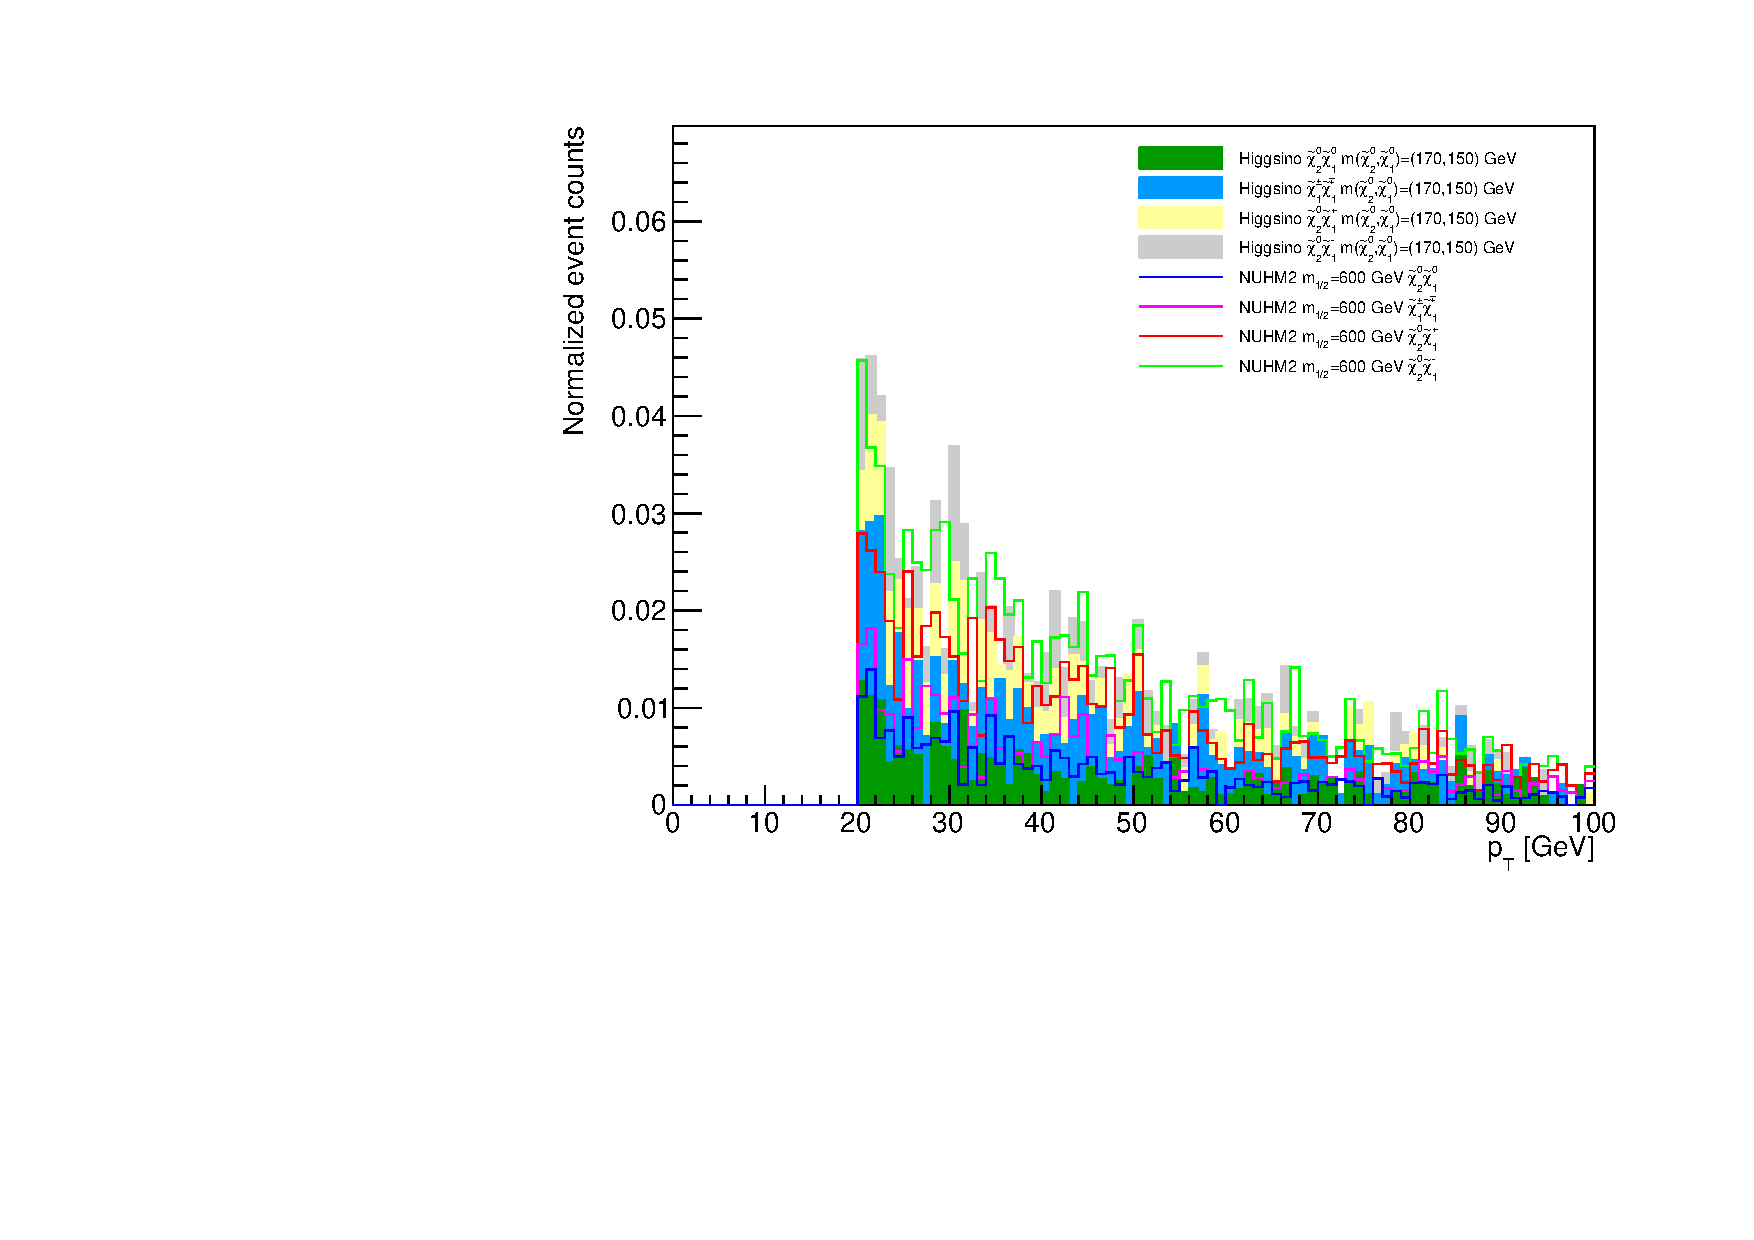
\includegraphics[scale=0.35]{signalBjets_pt.pdf}
            \caption{The signal $b$-jets \pt.}
        \end{subfigure}
        \begin{subfigure}[b]{0.48\textwidth}
            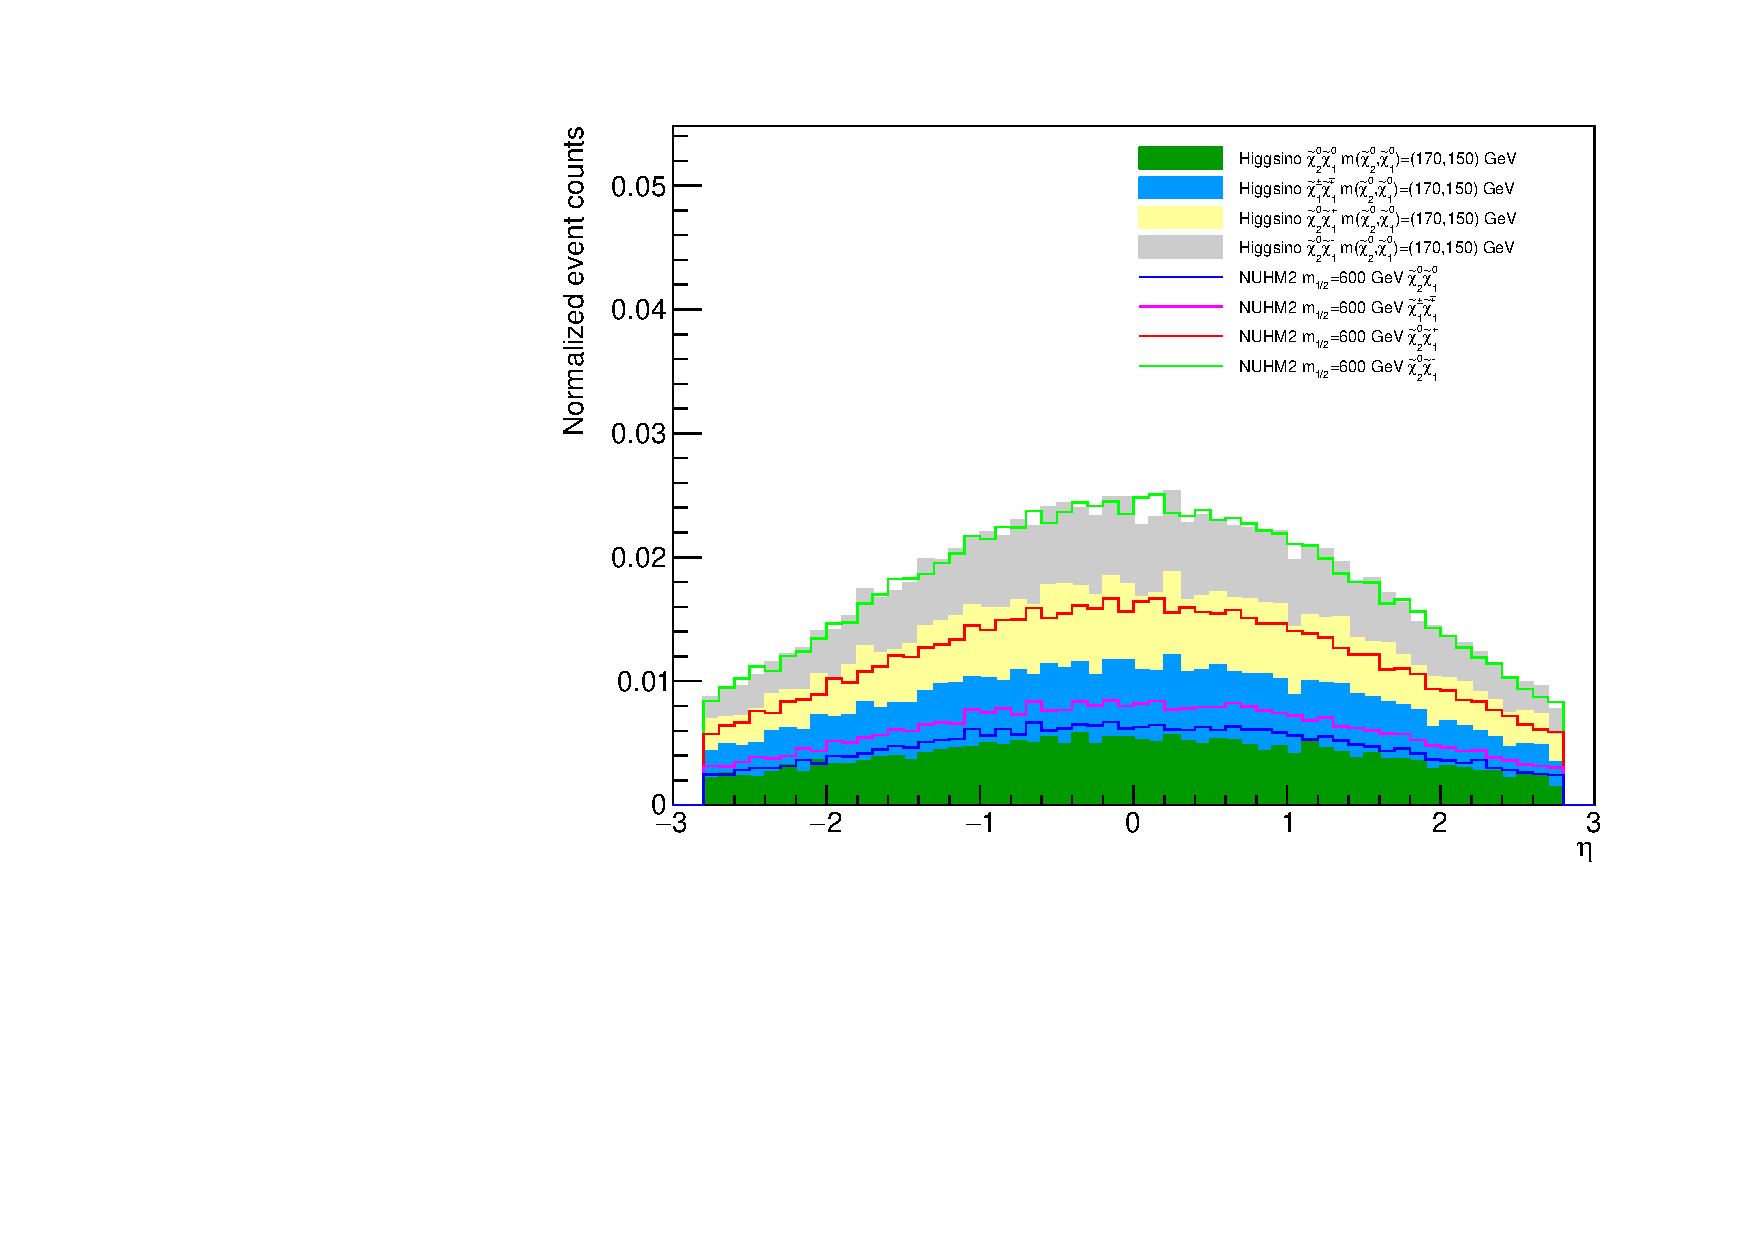
\includegraphics[scale=0.35]{signalJets_eta.pdf}
            \caption{The signal jets $\eta$.}
        \end{subfigure}
        \begin{subfigure}[b]{0.48\textwidth}
            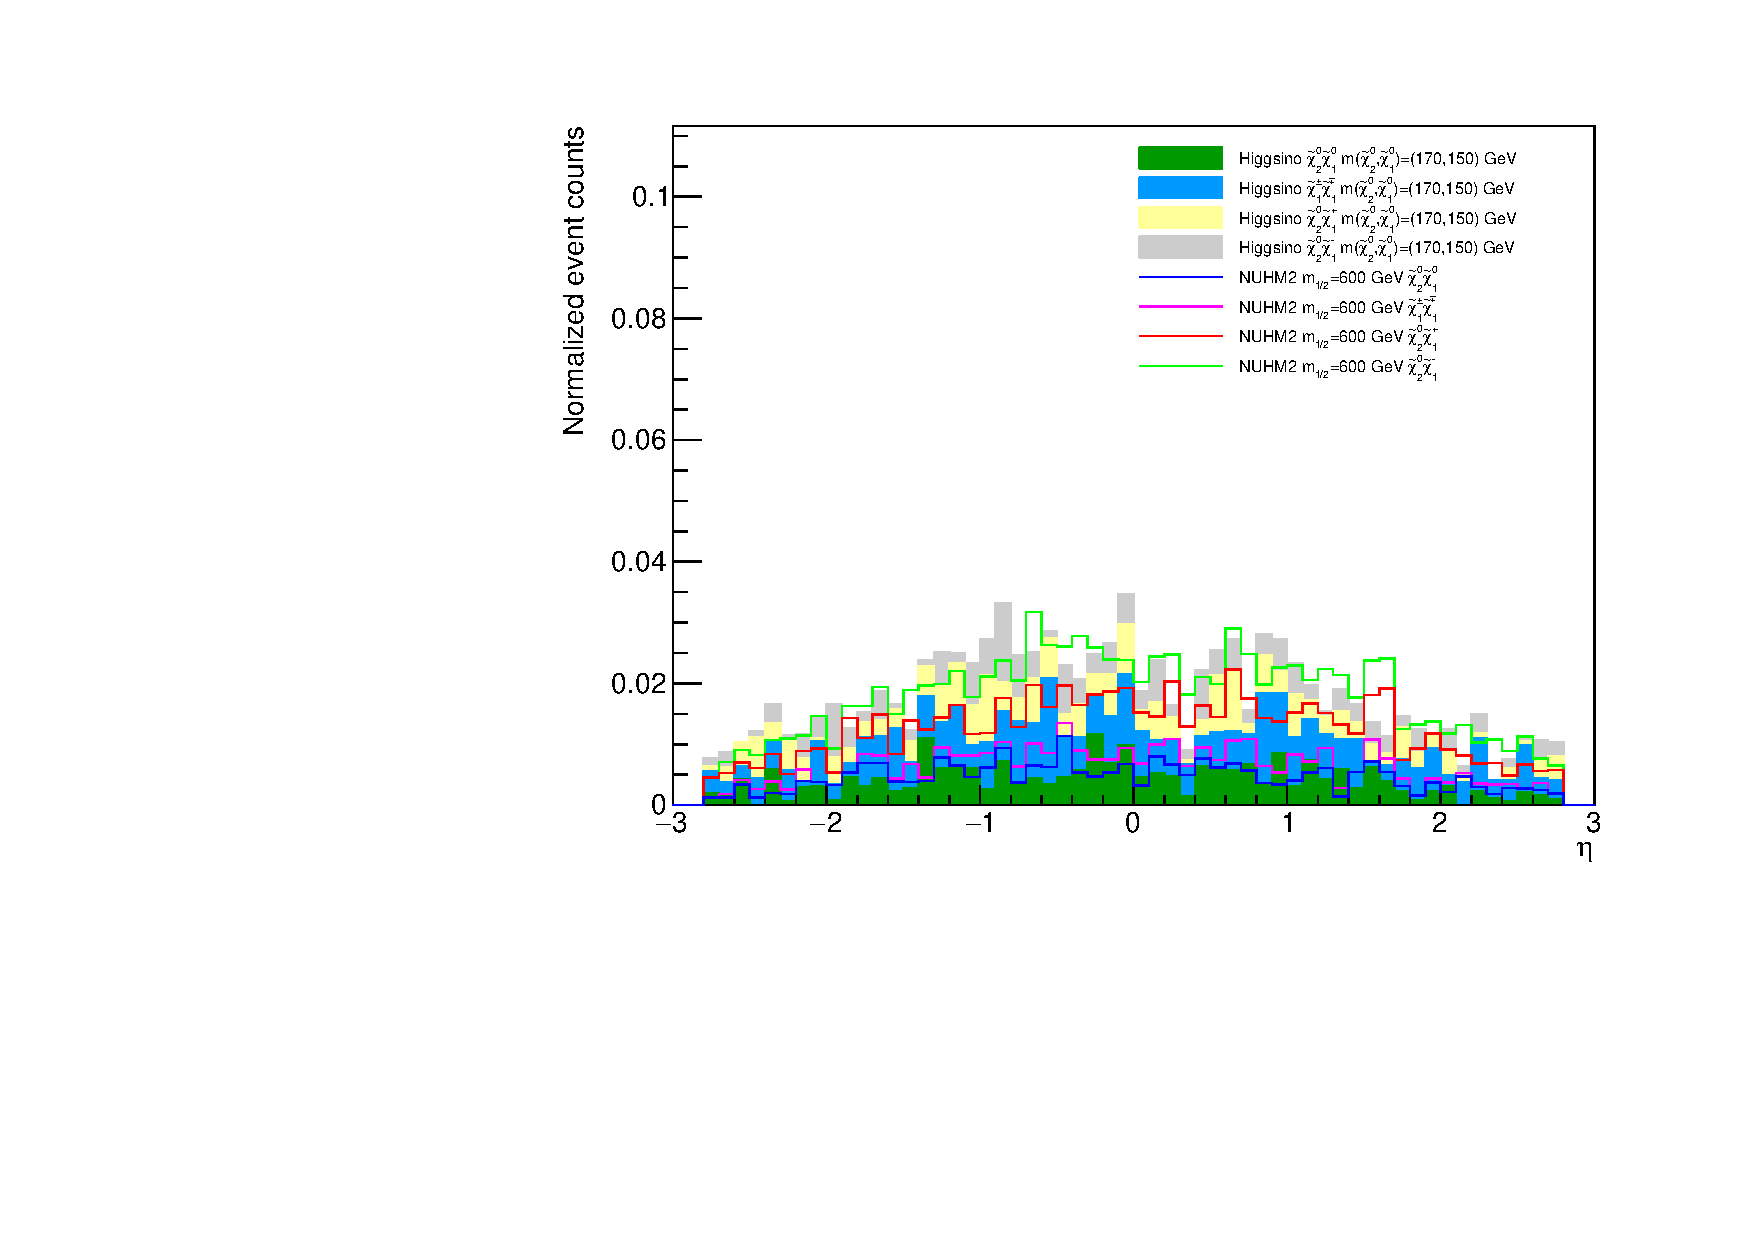
\includegraphics[scale=0.35]{signalBjets_eta.pdf}
            \caption{The signal $b$-jets $\eta$.}
        \end{subfigure}
        \begin{subfigure}[b]{0.48\textwidth}
            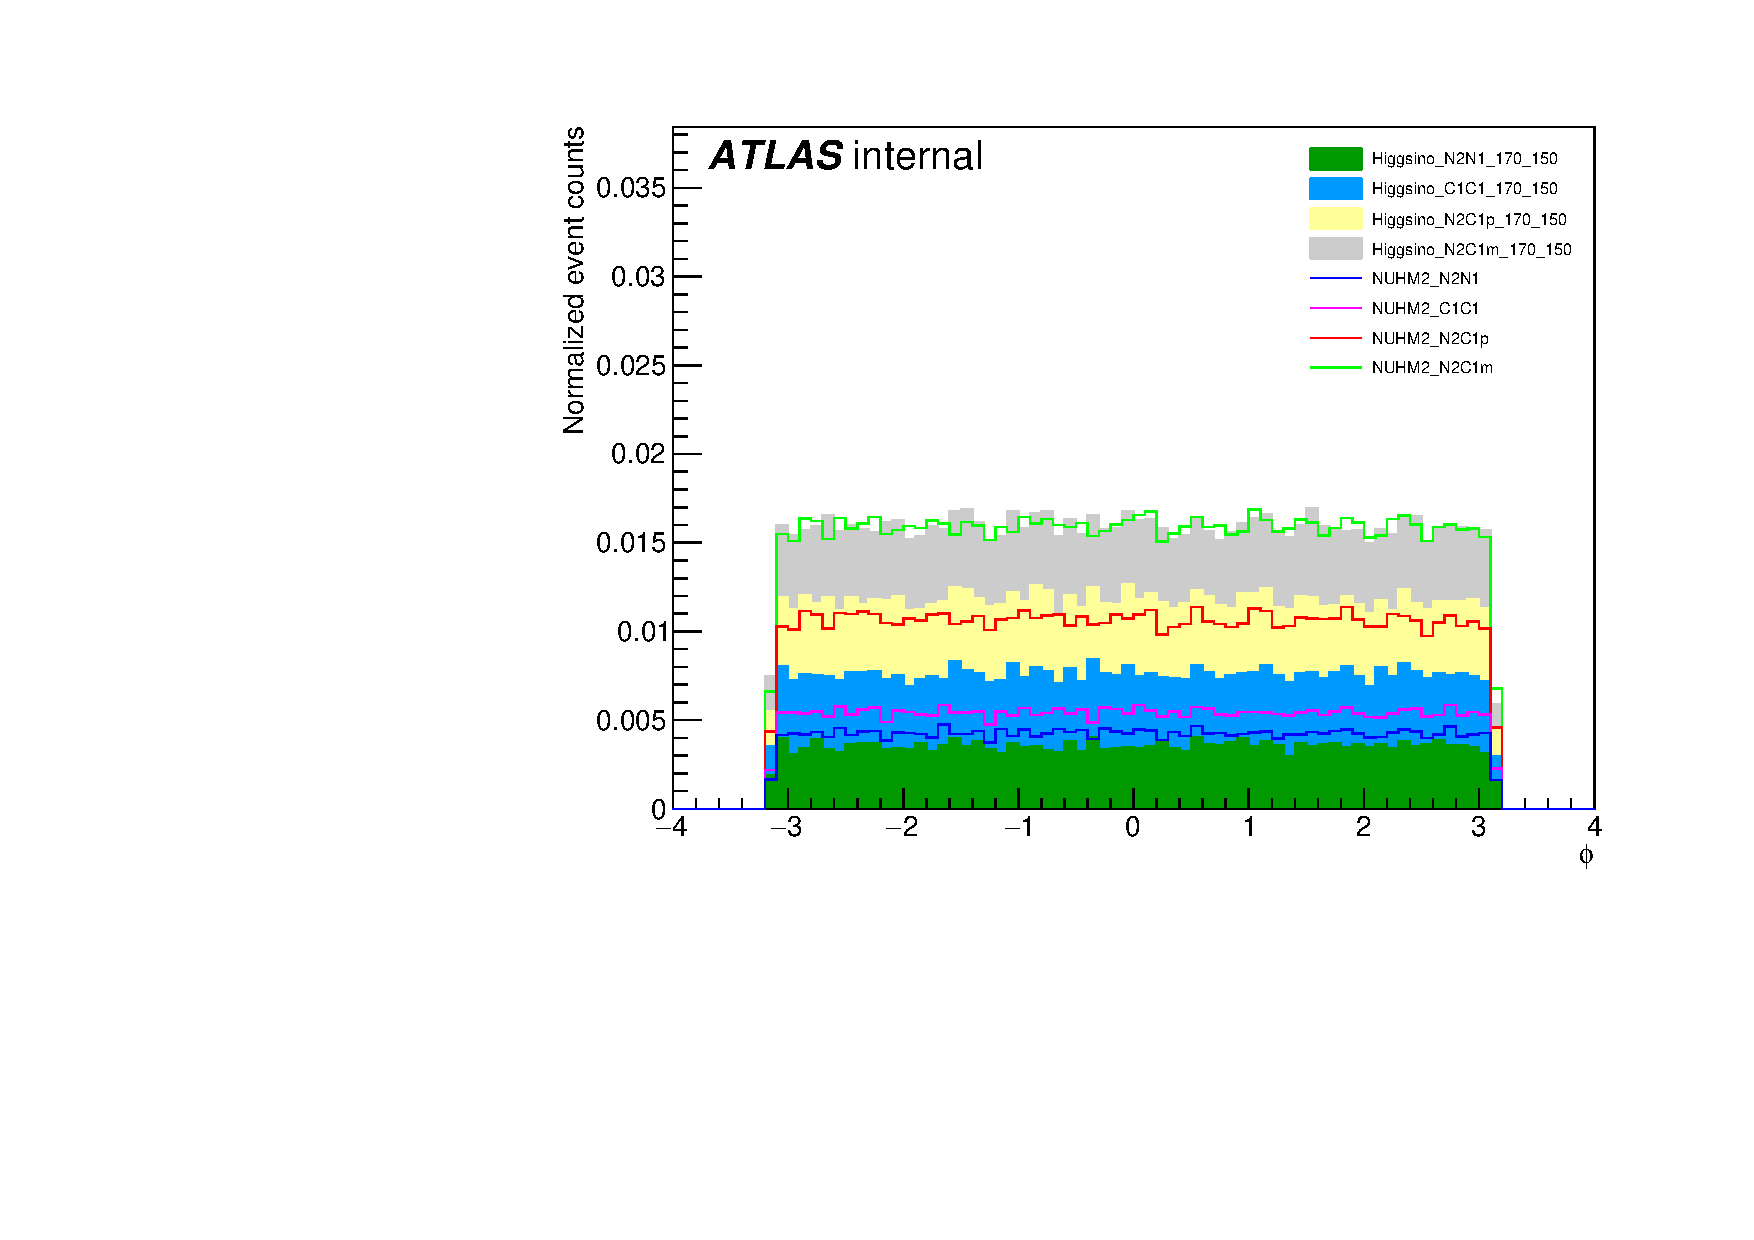
\includegraphics[scale=0.35]{signalJets_phi.pdf}
            \caption{The signal jets $\phi$.}
        \end{subfigure}
        \begin{subfigure}[b]{0.48\textwidth}
            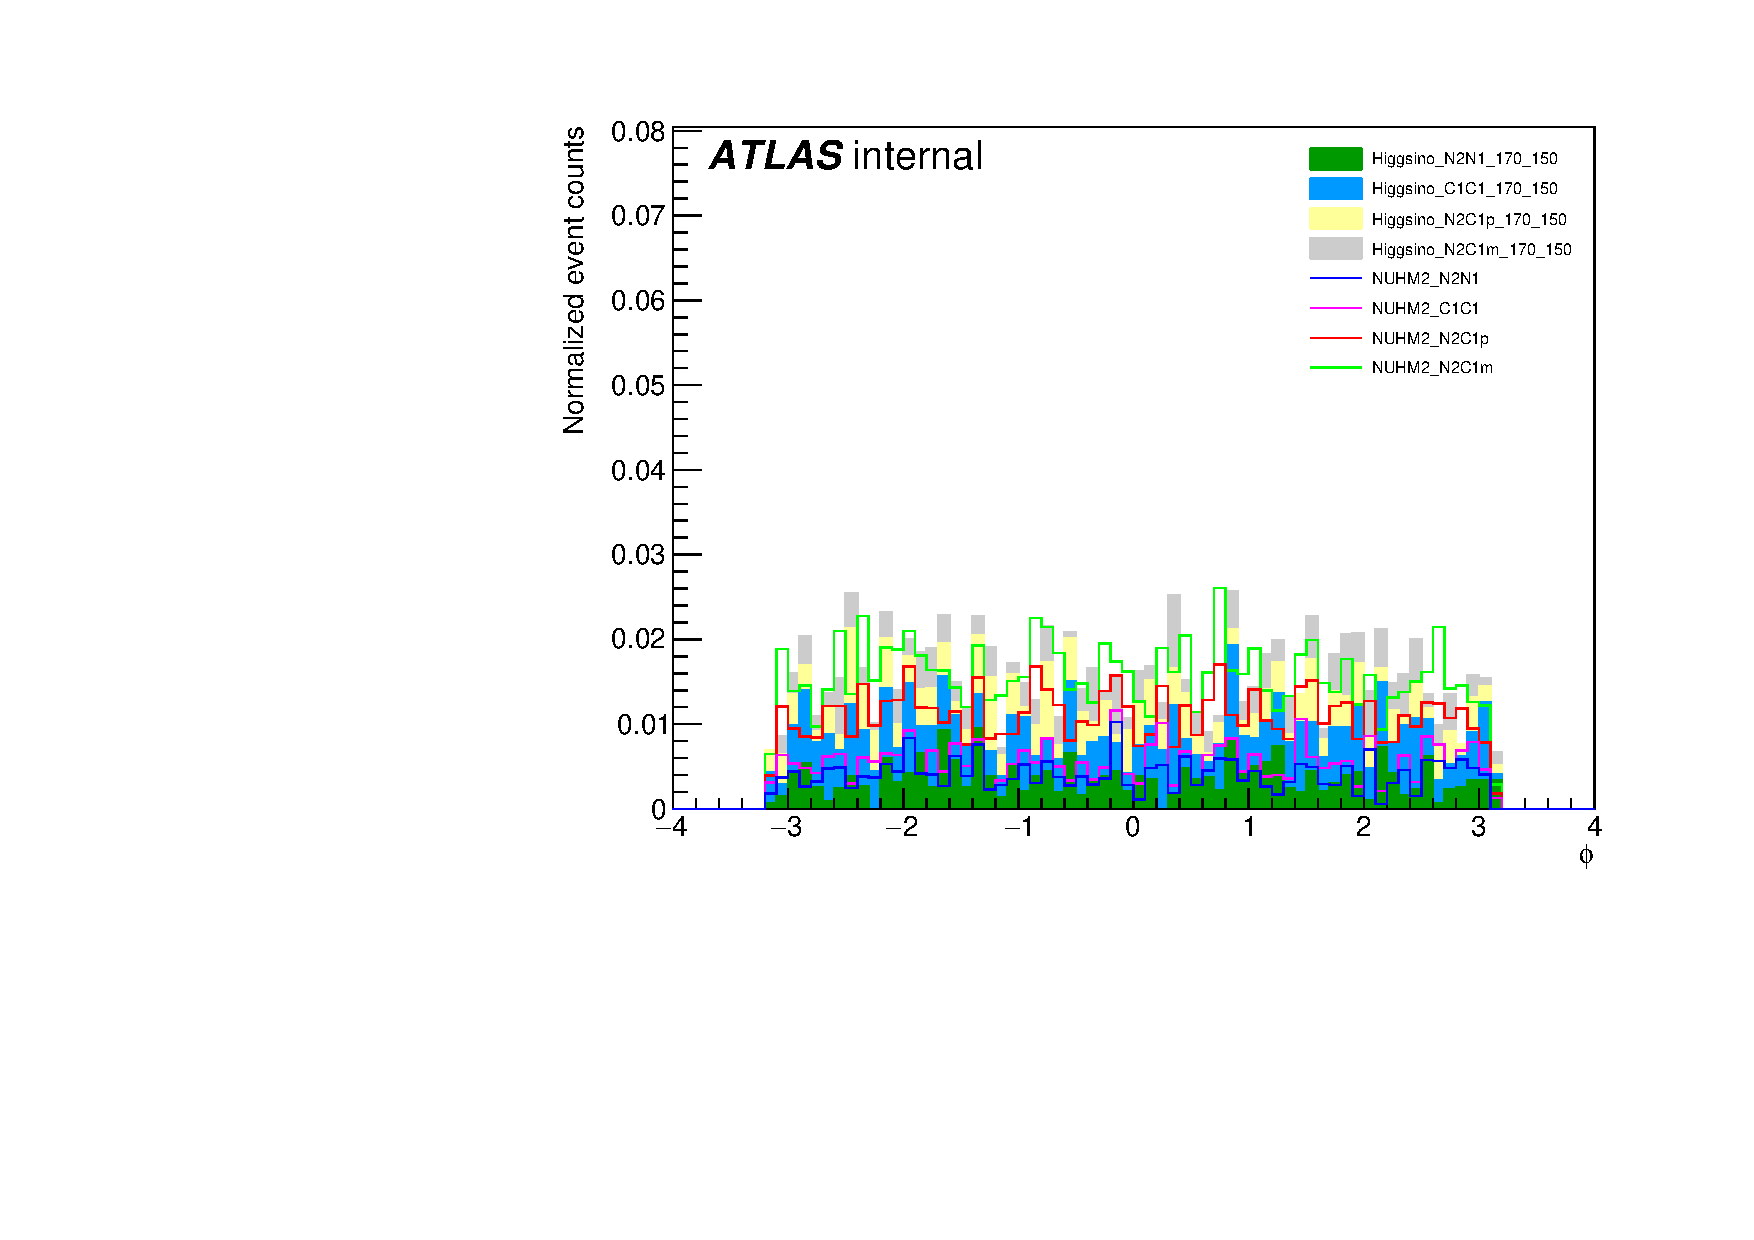
\includegraphics[scale=0.35]{signalBjets_phi.pdf}
            \caption{The signal $b$-jets $\phi$.}
        \end{subfigure}
    \end{center}
    \caption{The signal jets and the signal $b$-jets \pt, $\eta$, and $\phi$ distributions for the NUHM2 with $m_{1/2} = 600$~{\GeV} and the simplified Higgsino model with $m_{\widetilde{\chi}^{0}_{2}}=170$~{\GeV} and $m_{\widetilde{\chi}^{0}_{1}}=150$~{\GeV}.
    Four different production channels, $\widetilde{\chi}^{0}_{2}\widetilde{\chi}^{0}_{1}$, $\widetilde{\chi}^{0}_{2}\widetilde{\chi}^{+}_{1}$, $\widetilde{\chi}^{0}_{2}\widetilde{\chi}^{-}_{1}$, and $\widetilde{\chi}^{\pm}_{1}\widetilde{\chi}^{\mp}_{1}$, for the NUHM2 and the simplified Higgsino model are considered.
    The distributions of four productions are combined and normalized to equal area.}
    \label{fig:results_nuhm2_jets_bjets_pt_eta_phi}
\end{figure}

\begin{figure}[htbp]
    \begin{center}
        \begin{subfigure}[b]{0.48\textwidth}
            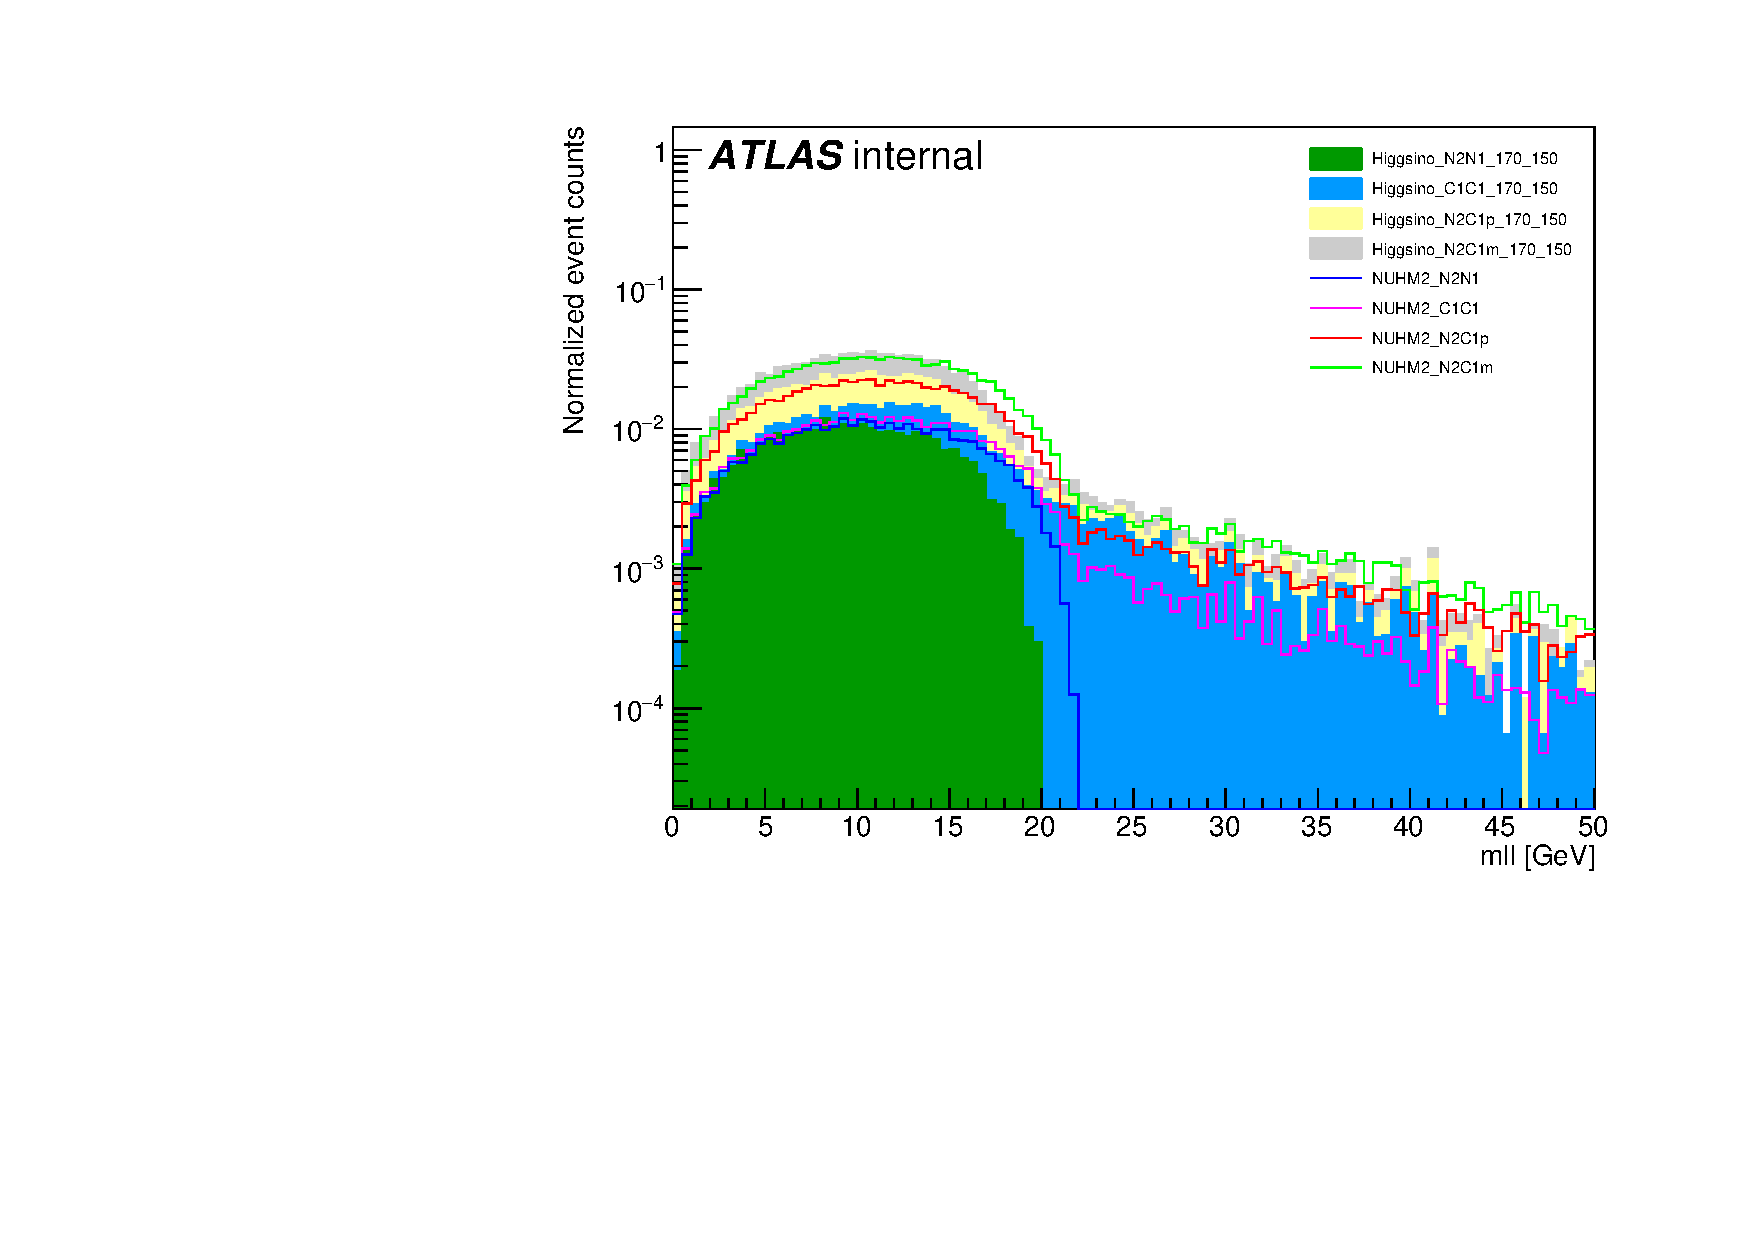
\includegraphics[scale=0.4]{mll.pdf}
            \caption{$M_{\ell\ell}$}
        \end{subfigure}
        \begin{subfigure}[b]{0.48\textwidth}
            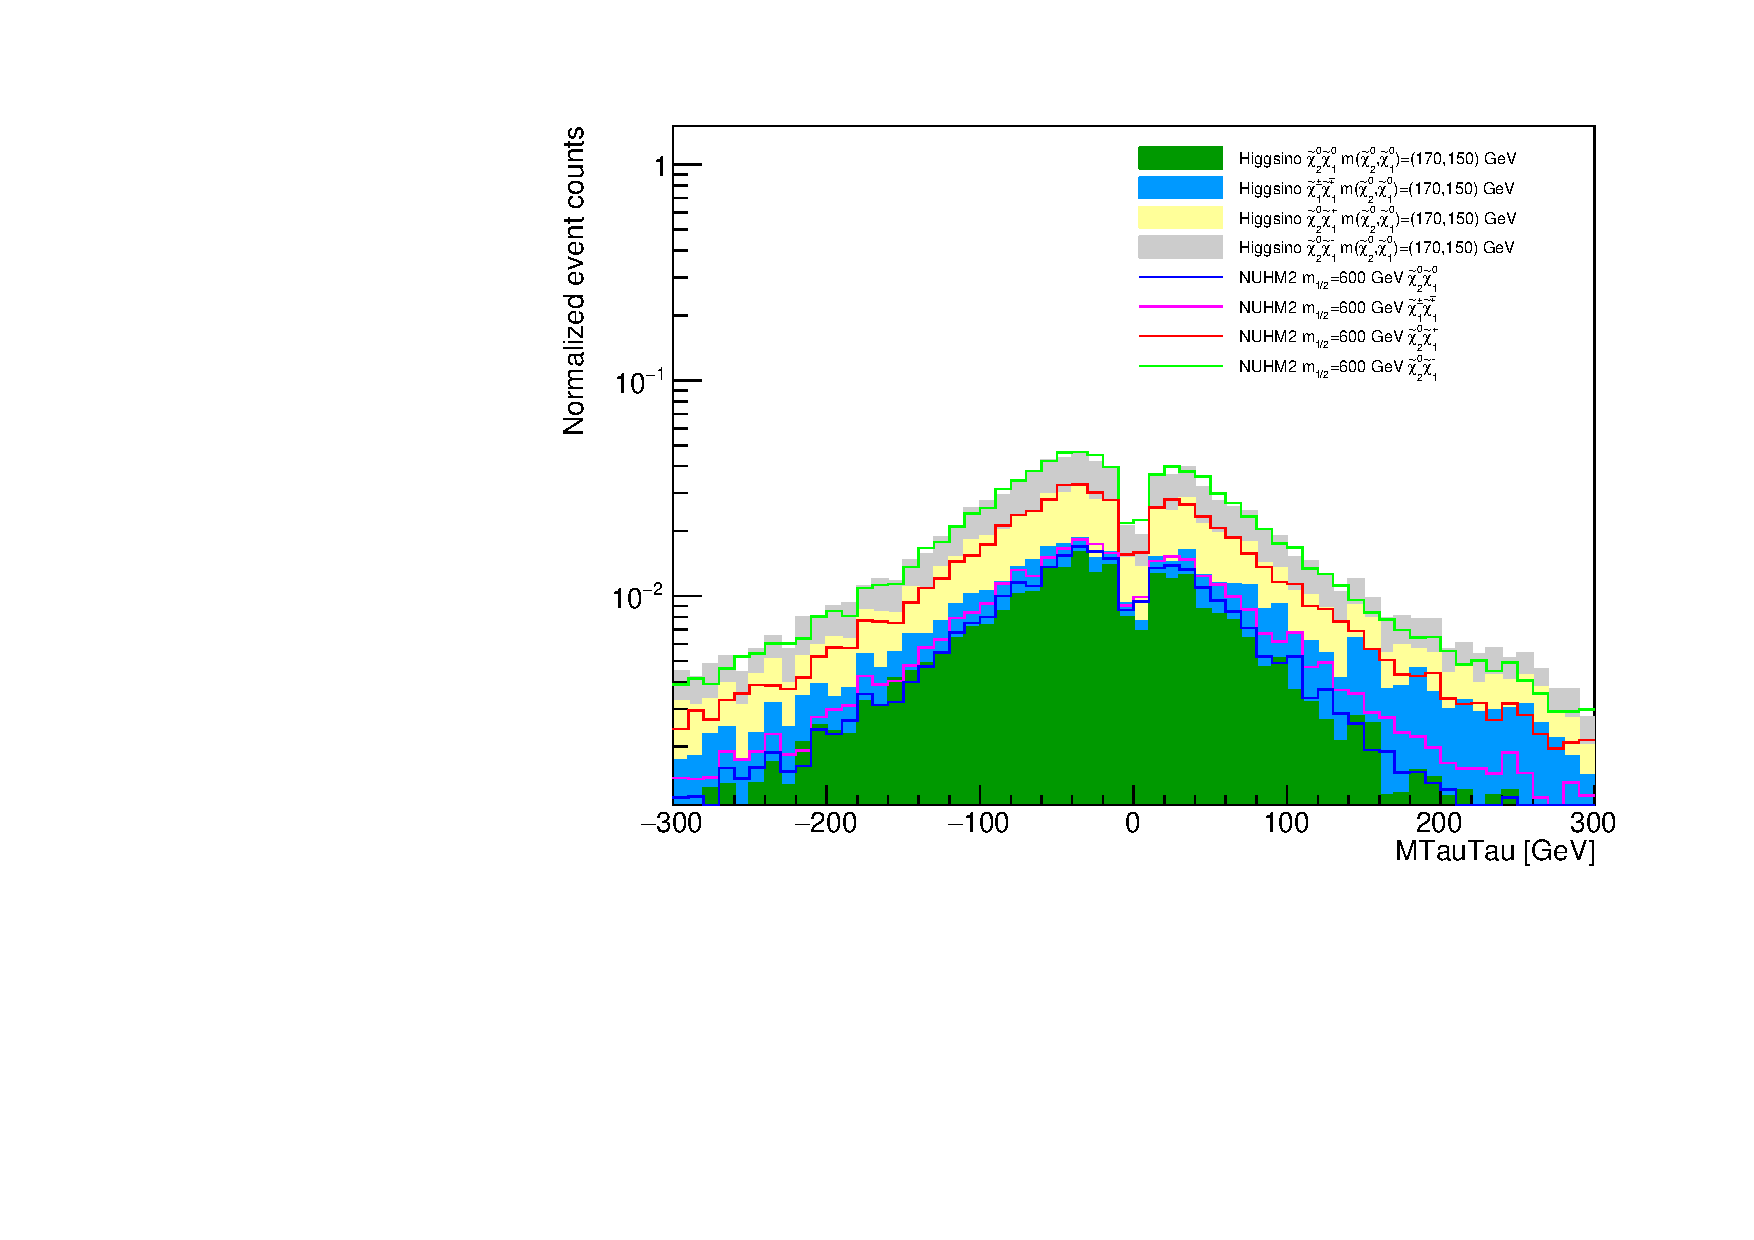
\includegraphics[scale=0.4]{MTauTau.pdf}
            \caption{$M_{\tau\tau}$}
        \end{subfigure}
        \begin{subfigure}[b]{0.48\textwidth}
            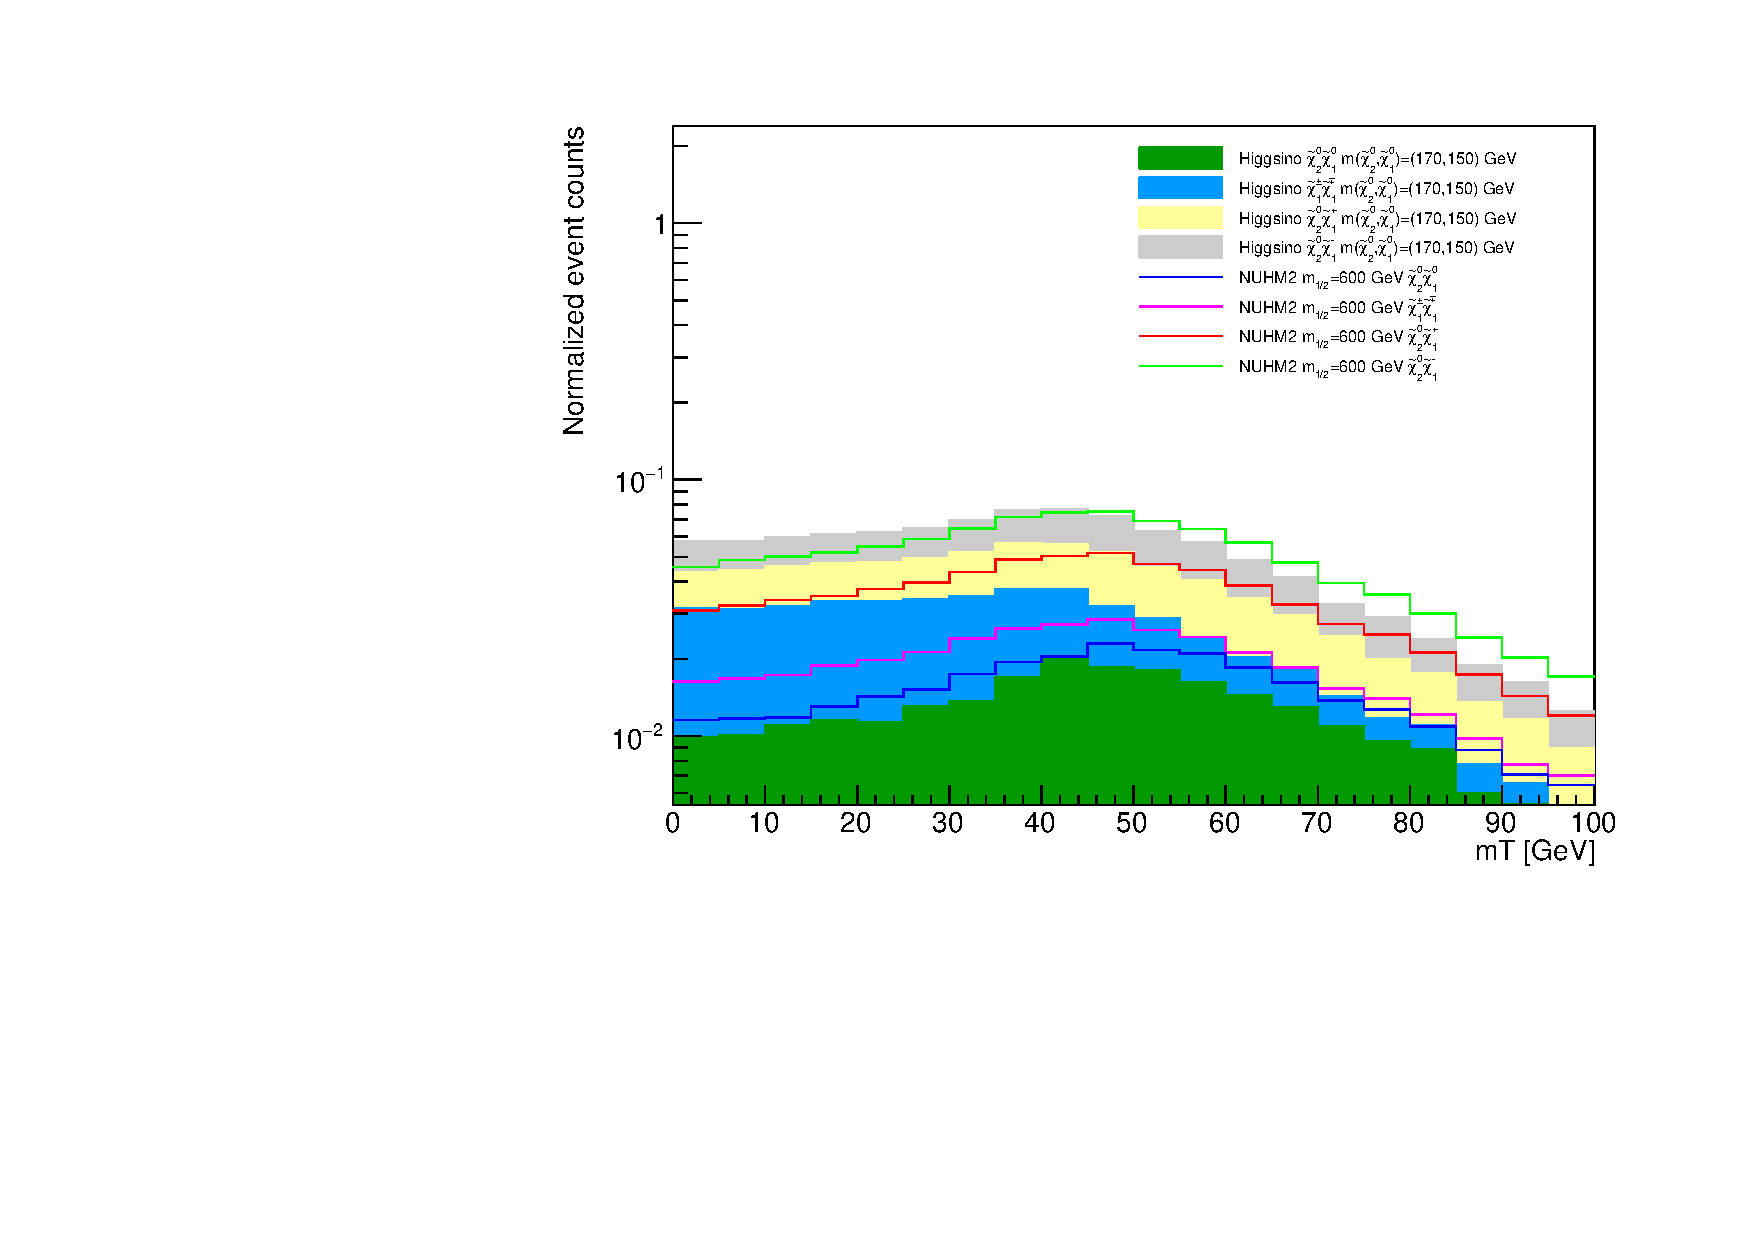
\includegraphics[scale=0.4]{mT.pdf}
            \caption{$M_{T}$}
        \end{subfigure}
        \begin{subfigure}[b]{0.48\textwidth}
            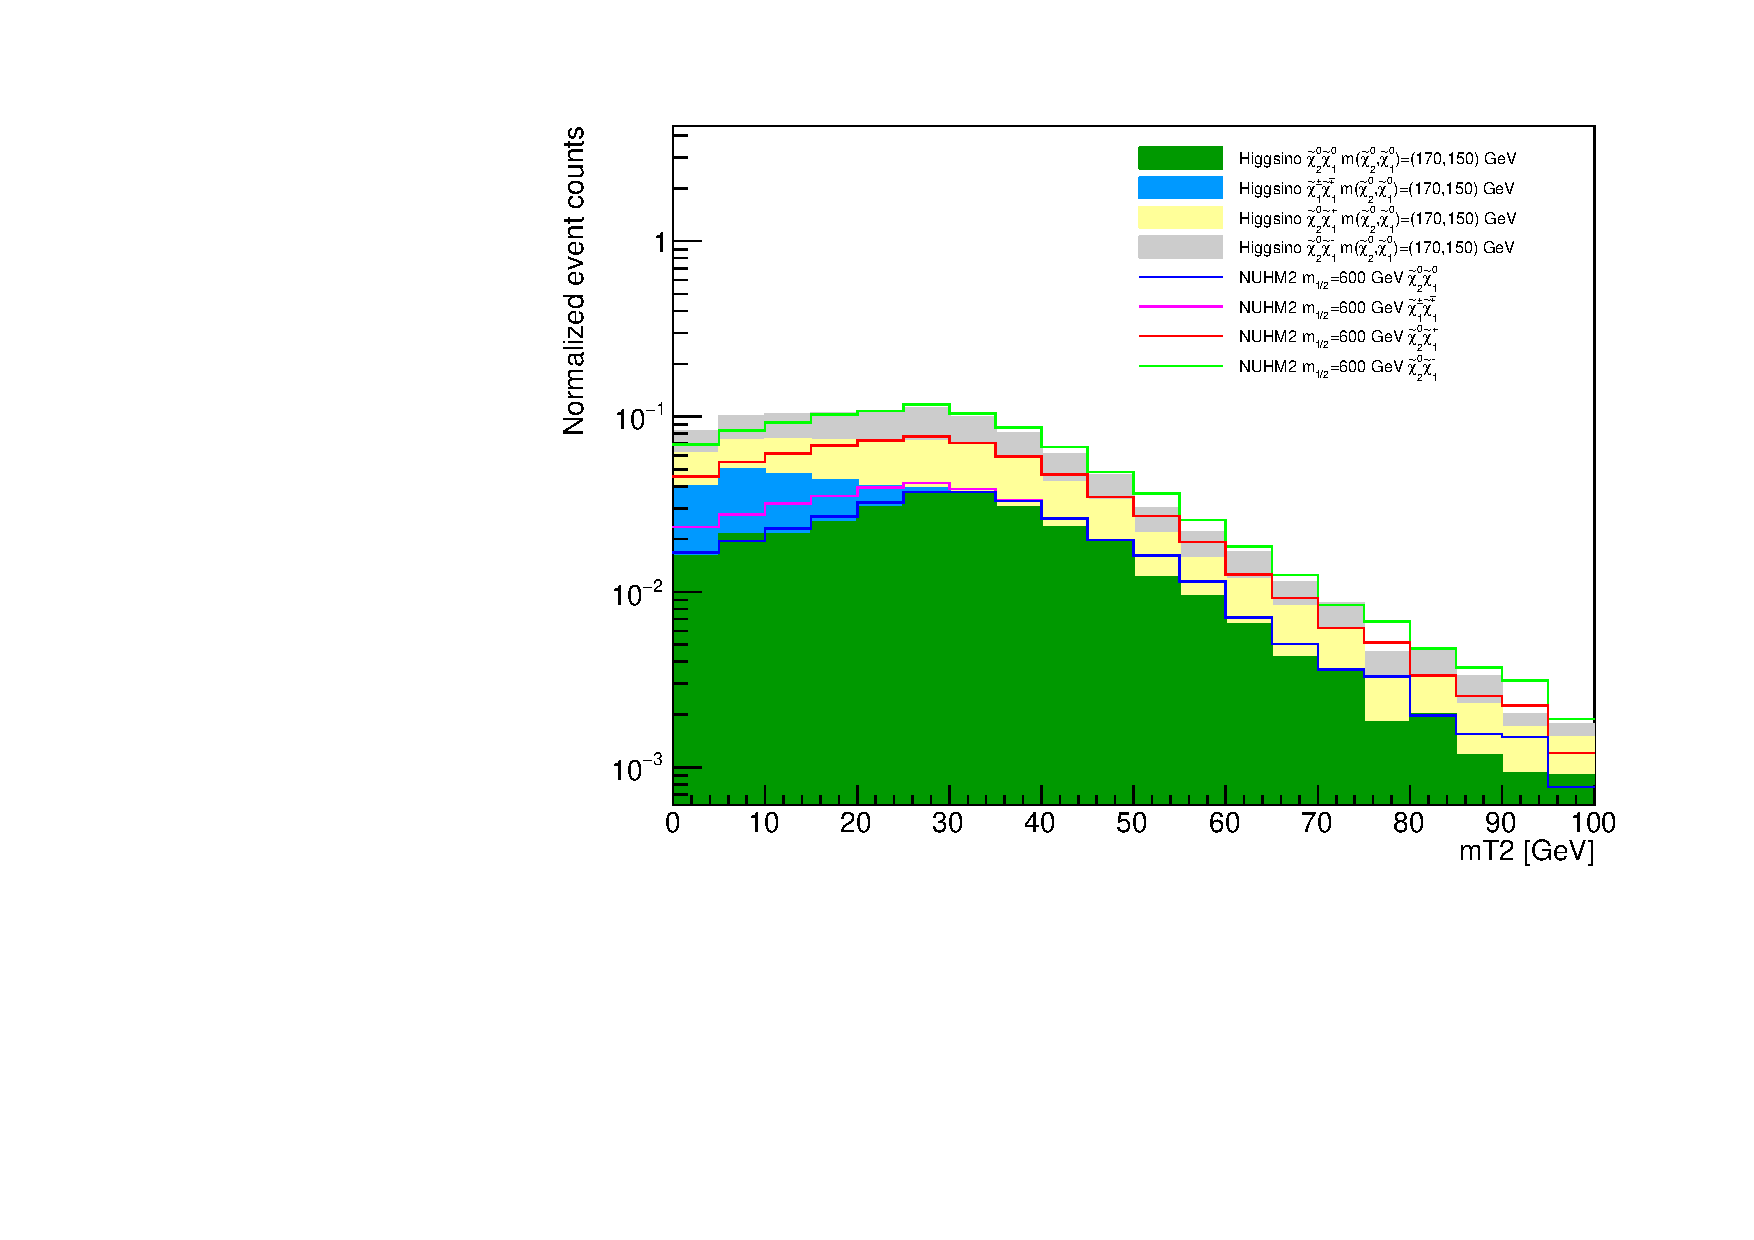
\includegraphics[scale=0.4]{mT2.pdf}
            \caption{$M_{T2}$}
        \end{subfigure}
    \end{center}
    \caption{The invariant mass $M_{\ell\ell}$ and $M_{\tau\tau}$ distributions and the transverse mass $M_\mathrm{T}$ and $M_\mathrm{T2}$ distributions.
    The first two leading baseline leptons are used to calculate the $M_{\ell\ell}$ which contains a hump and a tail region.
    The $\widetilde{\chi}^{0}_{2} \widetilde{\chi}^{0}_{1}$ contributes to the hump only and the tail is contributed by the decay products containing the chargino $\widetilde{\chi}^{\pm}_{1}$.
    The Eq.~(\ref{eq:event_mtautau}) is used to calculate the di-tau invariant mass $M_{\tau\tau}$.
    The first or first two leading signal leptons and \met are used to evaluate the transverse mass $M_\mathrm{T}$ and $M_\mathrm{T2}$, respectively.
    Four different production channels, $\widetilde{\chi}^{0}_{2}\widetilde{\chi}^{0}_{1}$, $\widetilde{\chi}^{0}_{2}\widetilde{\chi}^{+}_{1}$, $\widetilde{\chi}^{0}_{2}\widetilde{\chi}^{-}_{1}$, and $\widetilde{\chi}^{\pm}_{1}\widetilde{\chi}^{\mp}_{1}$, for the NUHM2 and the simplified Higgsino model are considered.
    The distributions of four productions are combined and normalized to equal area.}
    \label{fig:results_nuhm2_mll_mtautau_mT_mT2}
\end{figure}

\begin{figure}[htbp]
    \begin{center}
        \begin{subfigure}[b]{0.48\textwidth}
            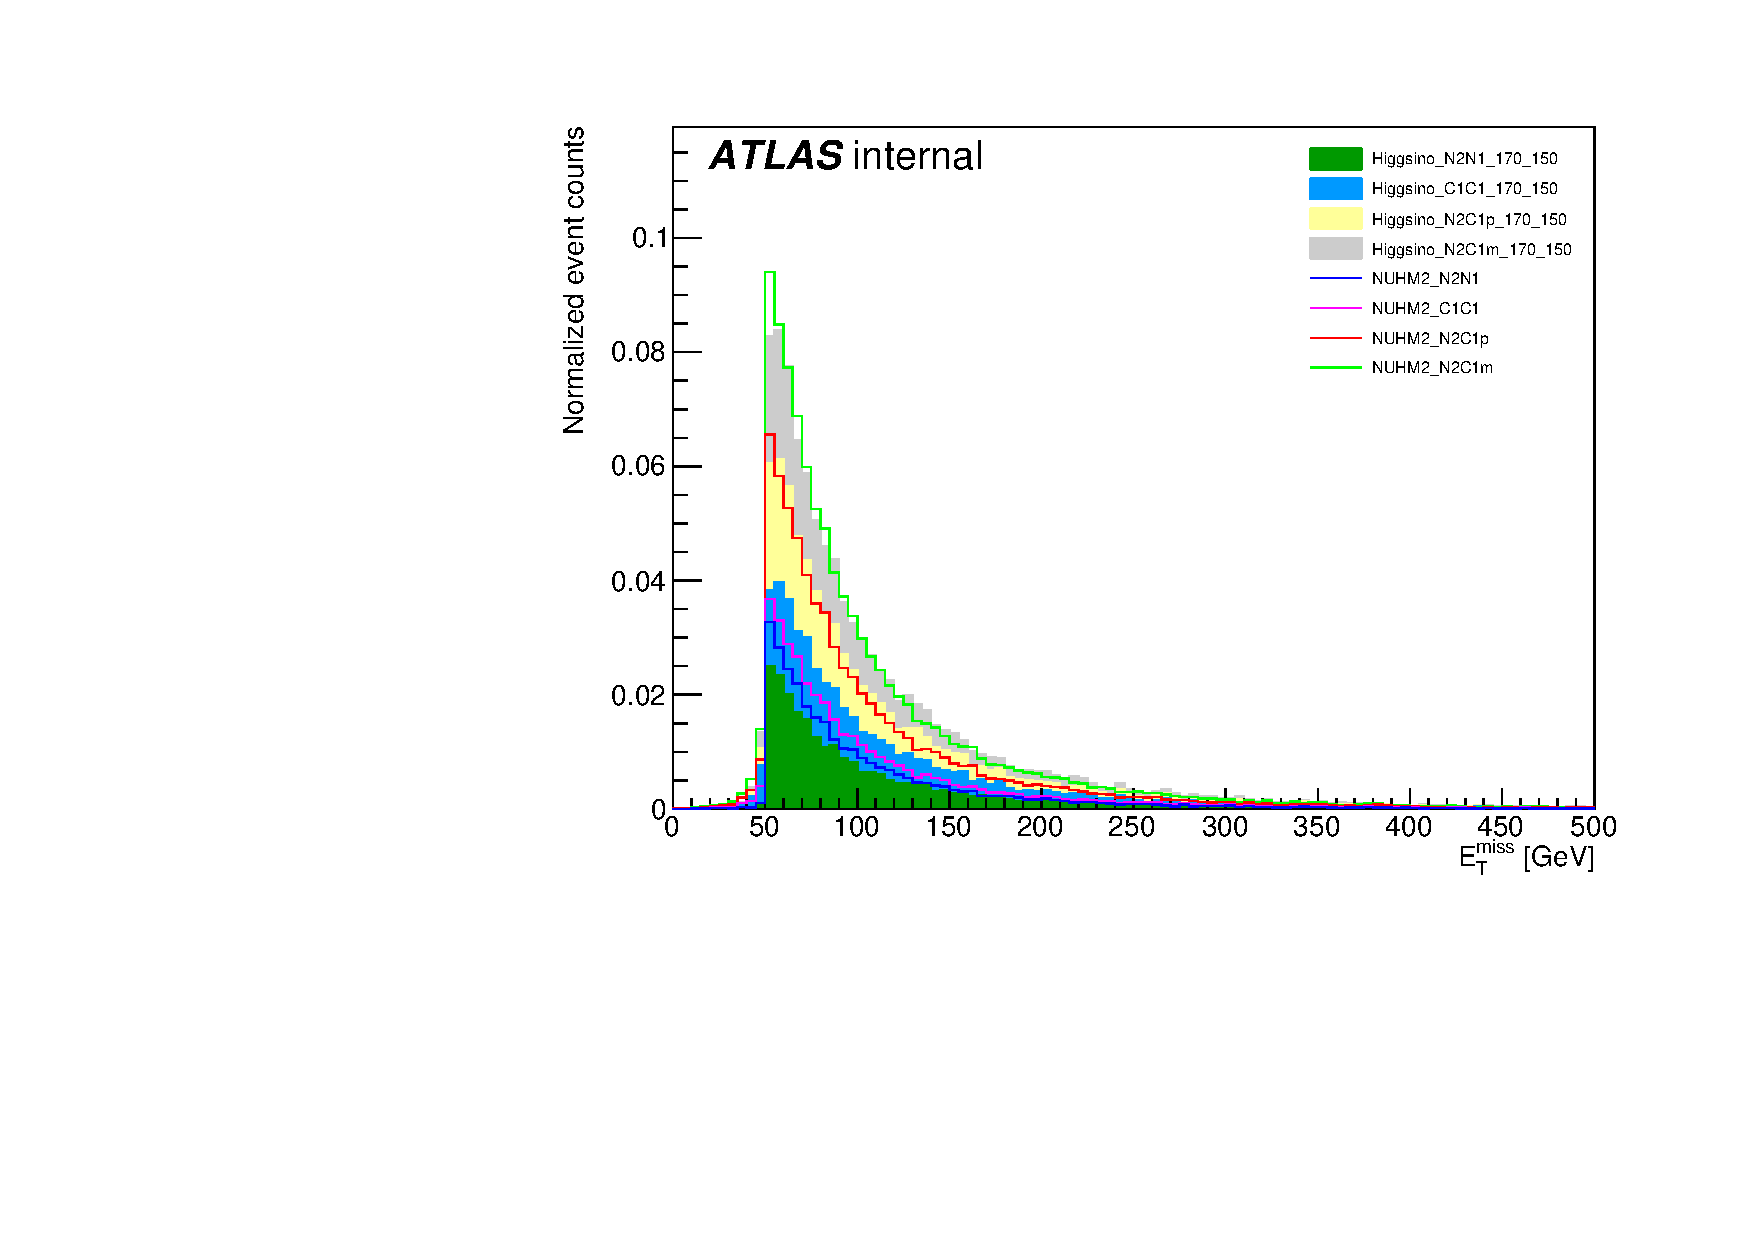
\includegraphics[scale=0.4]{met.pdf}
            \caption{\met}
        \end{subfigure}
        \begin{subfigure}[b]{0.48\textwidth}
            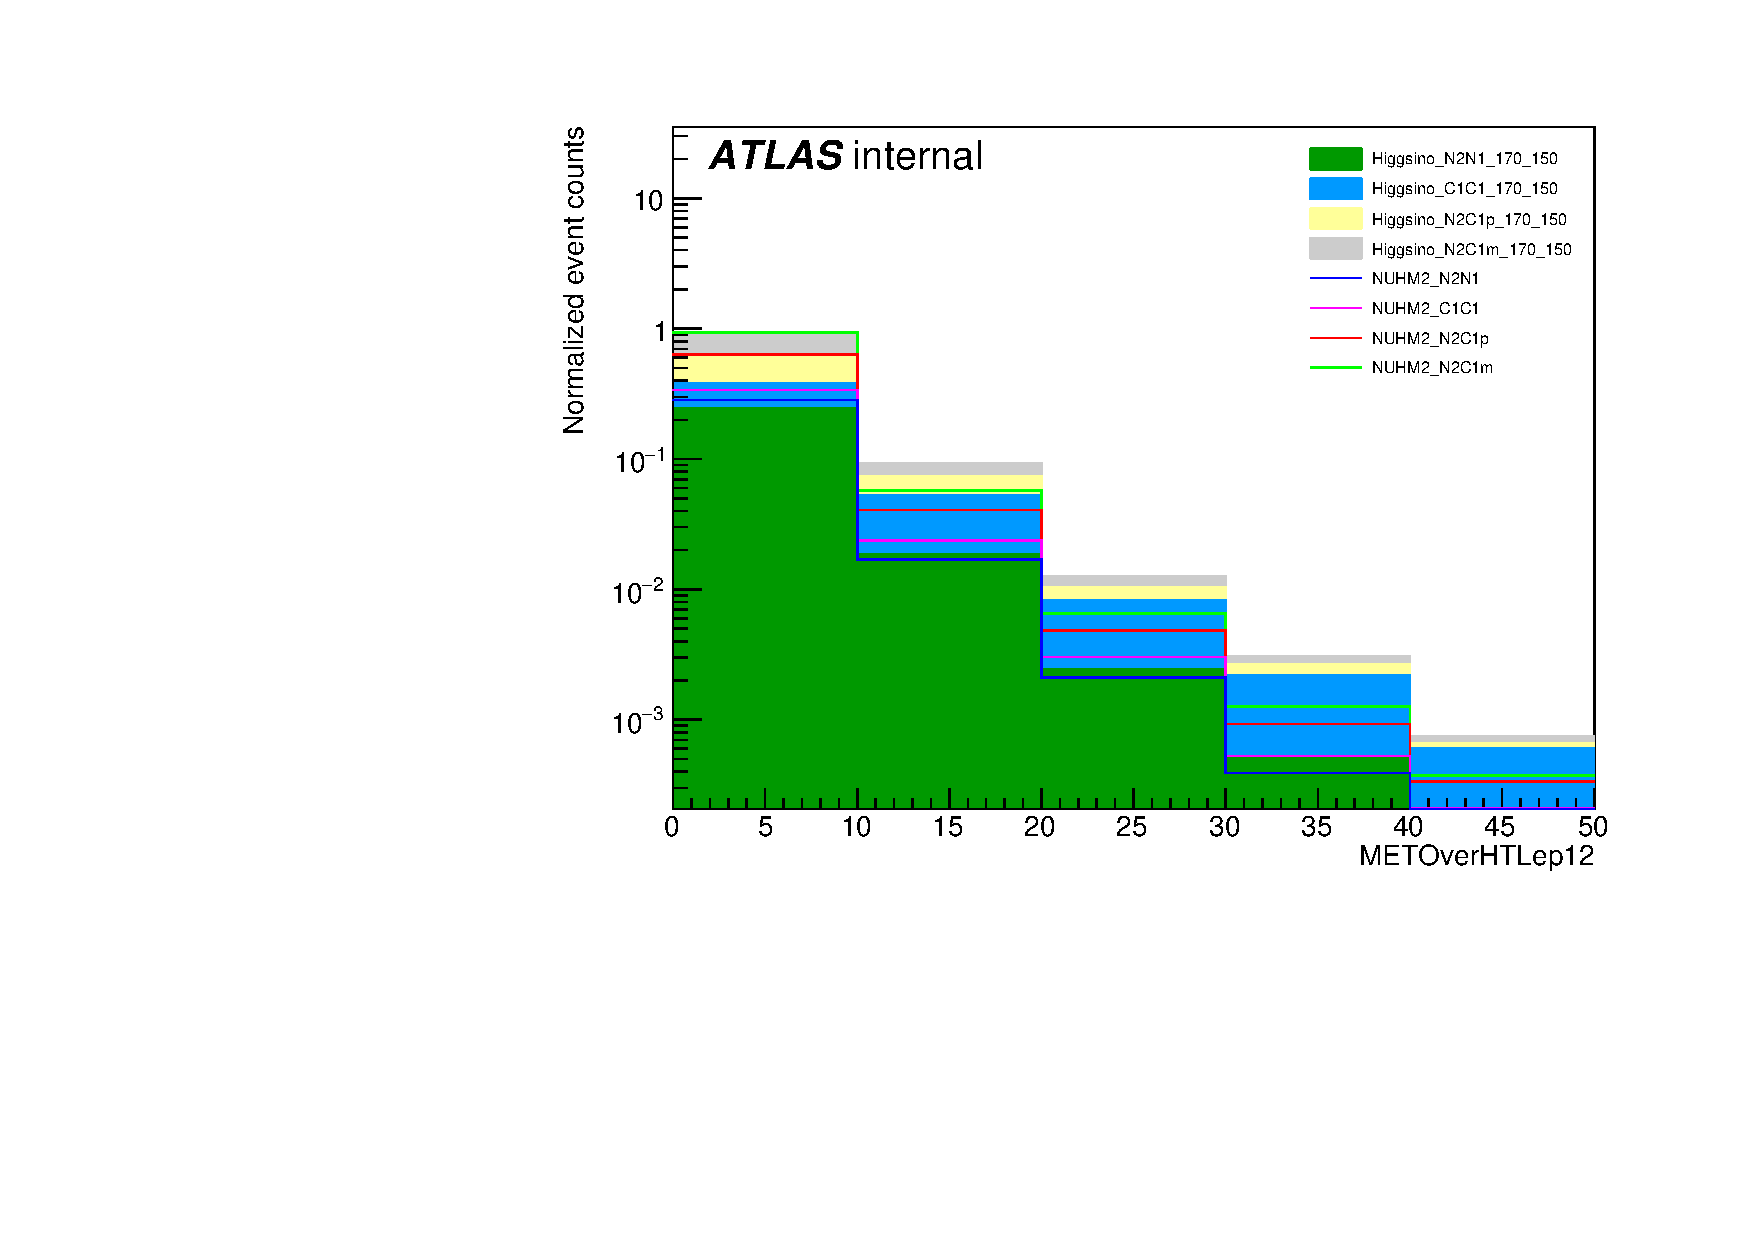
\includegraphics[scale=0.4]{METOverHTLep12.pdf}
            \caption{$\met/H_\mathrm{T}^\mathrm{lepton}$}
        \end{subfigure}
        \begin{subfigure}[b]{0.48\textwidth}
            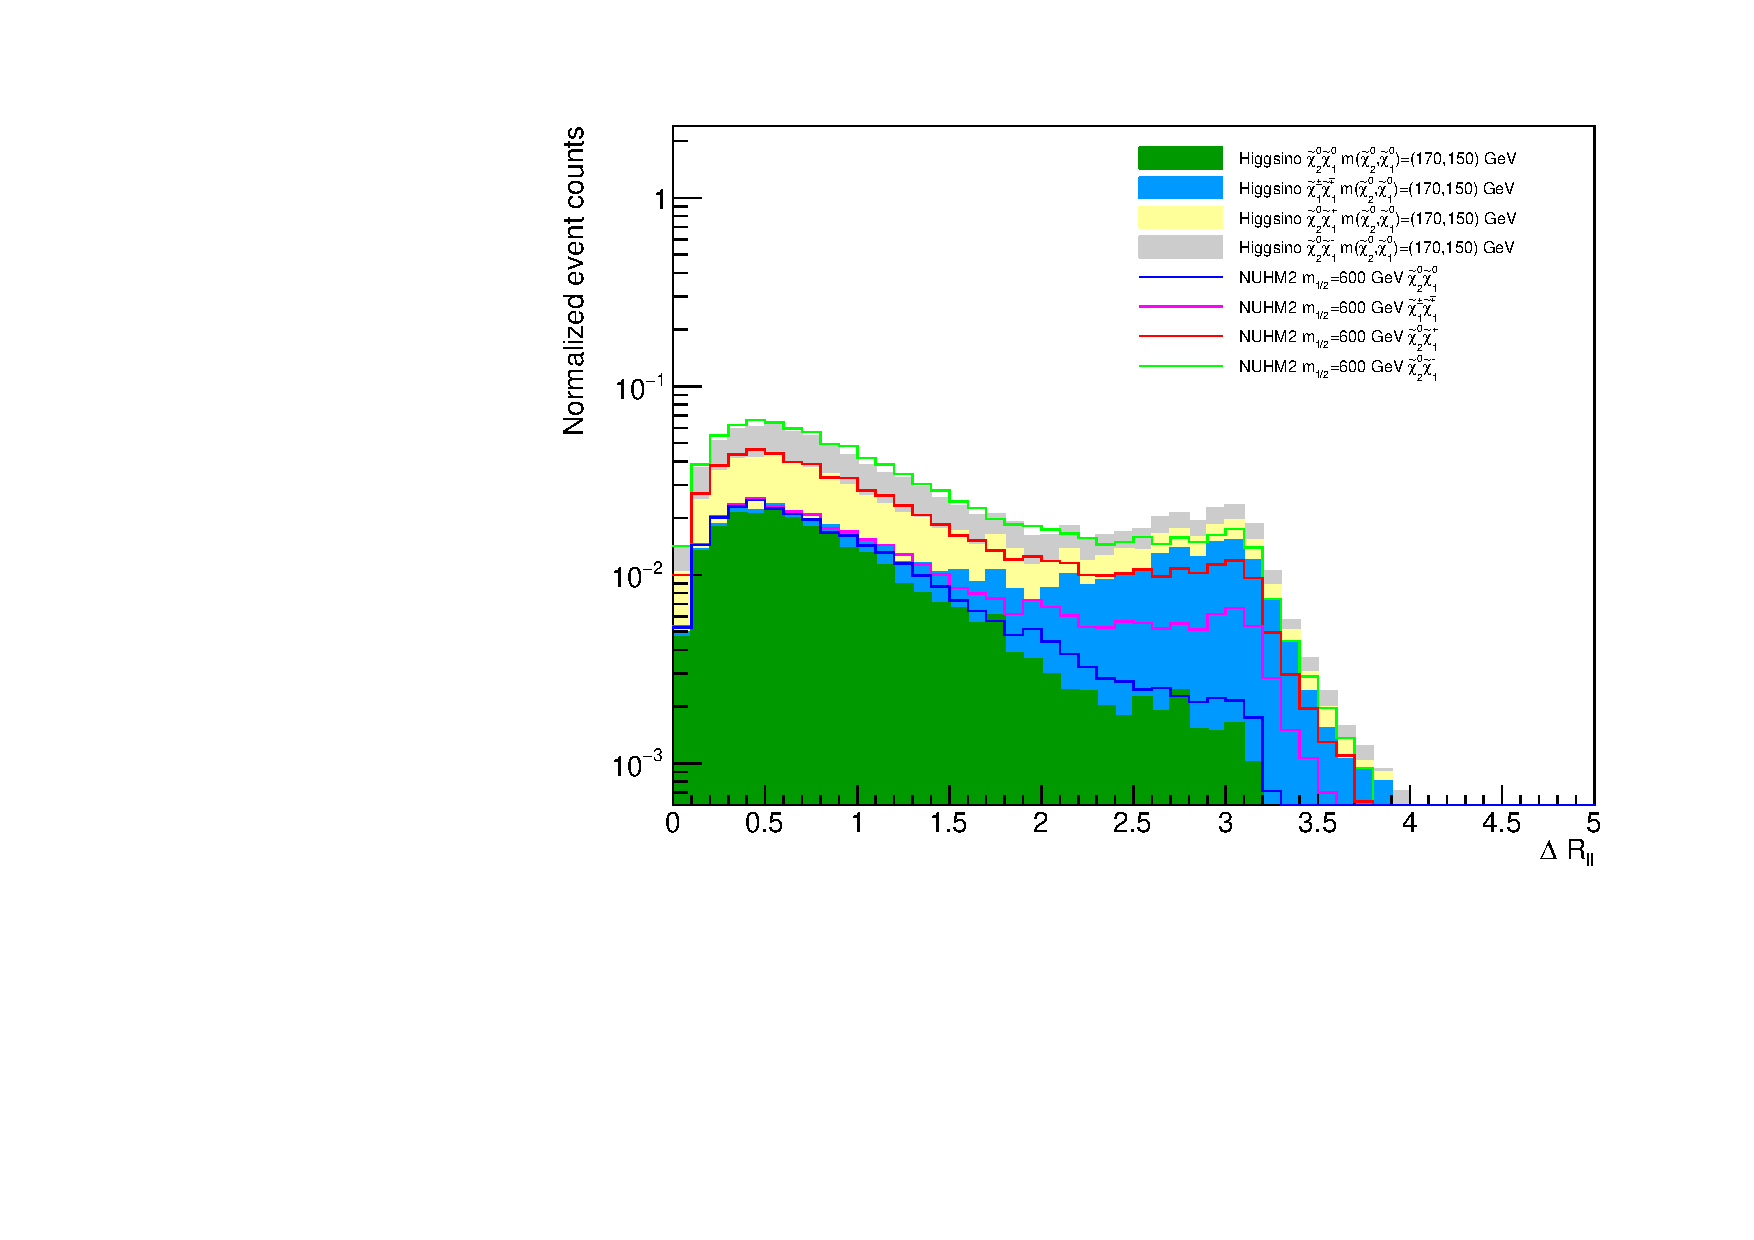
\includegraphics[scale=0.4]{Rll.pdf}
            \caption{$\Delta R(\ell_{1}, \ell_{2})$}
        \end{subfigure}
        \begin{subfigure}[b]{0.48\textwidth}
            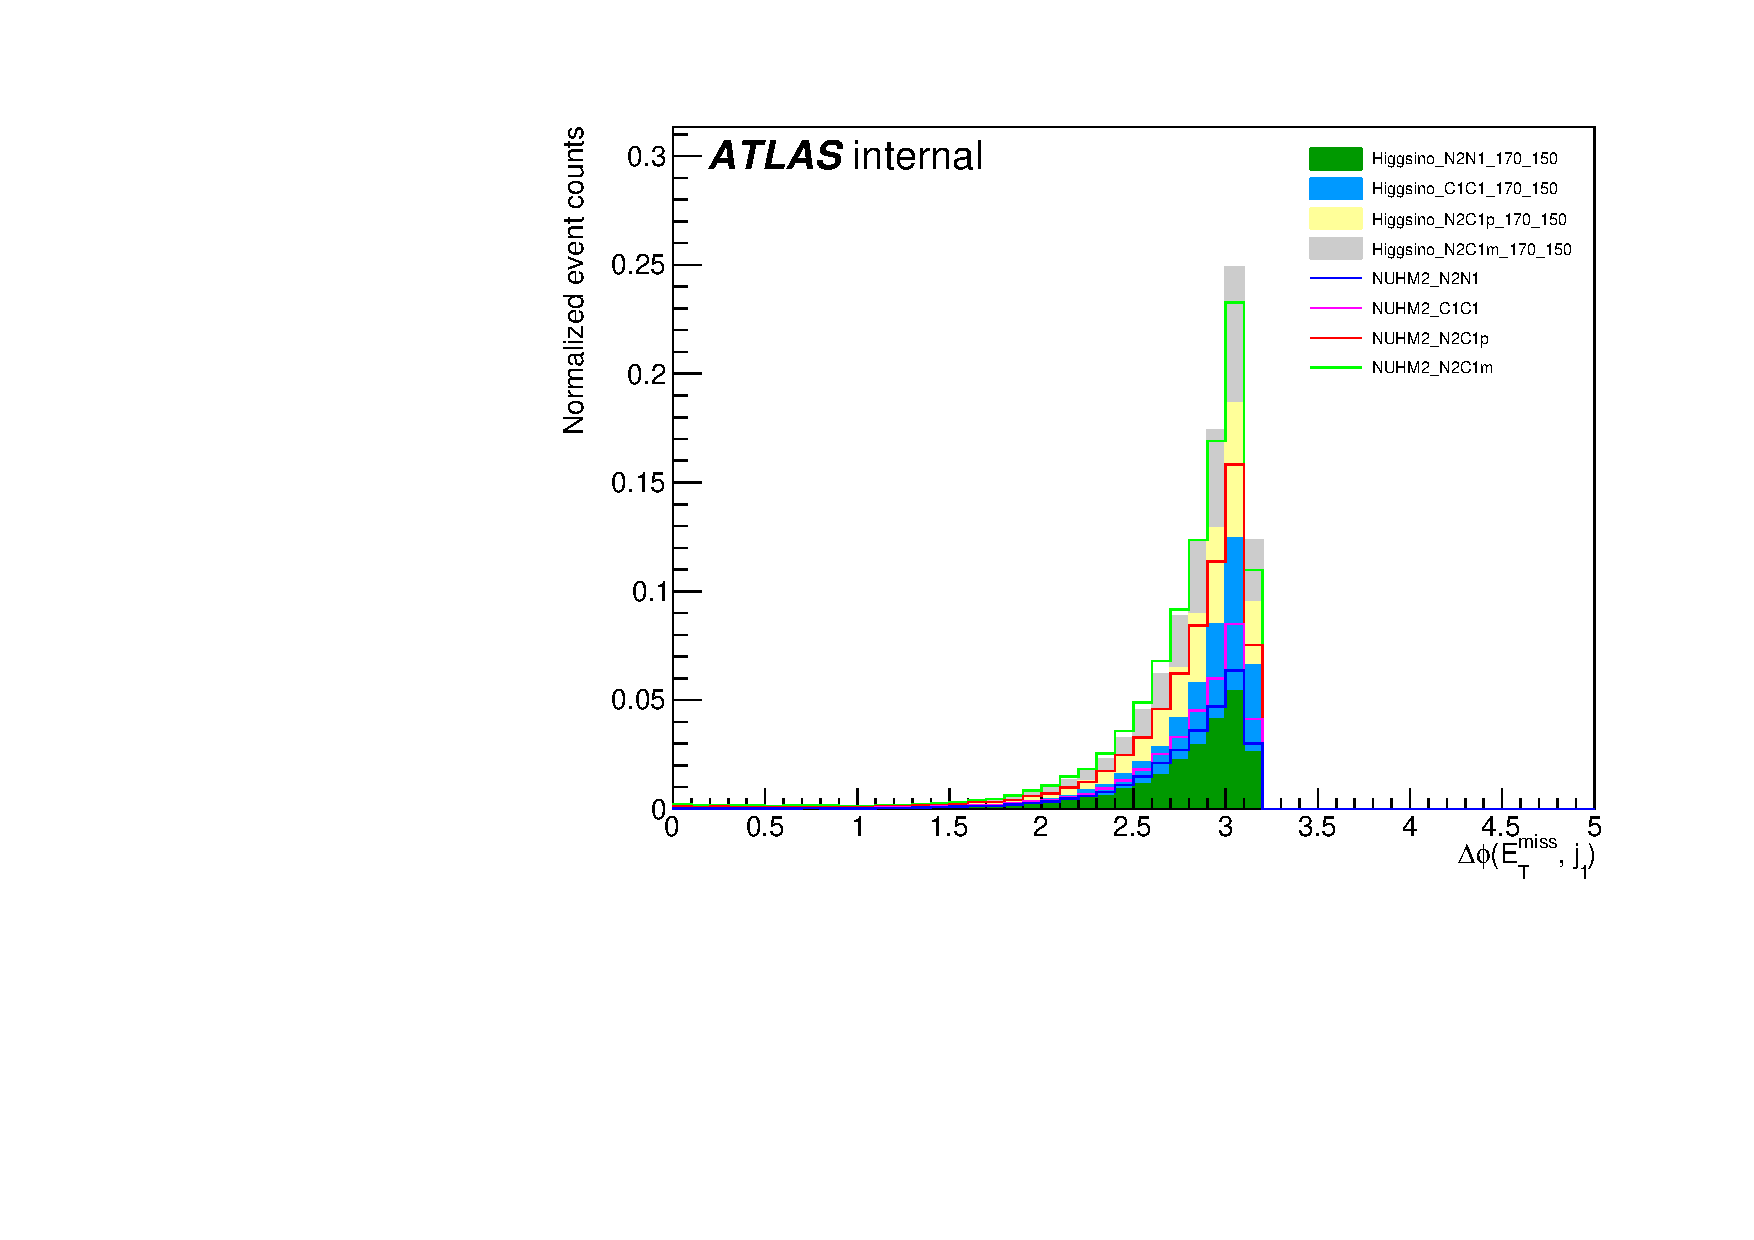
\includegraphics[scale=0.4]{dphiMin1.pdf}
            \caption{$\Delta \phi(\met, j_{1})$}
        \end{subfigure}
    \end{center}
    \caption{The \met, $\met/H_\mathrm{T}^\mathrm{lepton}$, $\Delta R(\ell_{1}, \ell_{2})$, and $\Delta \phi(\met, j_{1})$ distributions.
    The $H_\mathrm{T}^\mathrm{lepton}$ is the scalar sum of the first two leading baseline leptons \pt only.
    The distance $\Delta R(\ell_{1}, \ell_{2})$ is calculated by the first two leading baseline leptons and the $\Delta \phi(\met, j_{1})$ uses \met and first leading signal jet.
    Four different production channels, $\widetilde{\chi}^{0}_{2}\widetilde{\chi}^{0}_{1}$, $\widetilde{\chi}^{0}_{2}\widetilde{\chi}^{+}_{1}$, $\widetilde{\chi}^{0}_{2}\widetilde{\chi}^{-}_{1}$, and $\widetilde{\chi}^{\pm}_{1}\widetilde{\chi}^{\mp}_{1}$, for the NUHM2 and the simplified Higgsino model are considered.
    The distributions of four productions are combined and normalized to equal area.}
    \label{fig:results_nuhm2_met_METOverHTLep12_Rll_dphiMin1}
\end{figure}



%%%
%%%
%%%

\section{NUHM2 interpretation using the $m_{\ell \ell}$ re-weighting method}
\label{sec:results_mll_reweighting}



\begin{figure}[htbp]
    \begin{center}
        \begin{subfigure}[b]{0.48\textwidth}
            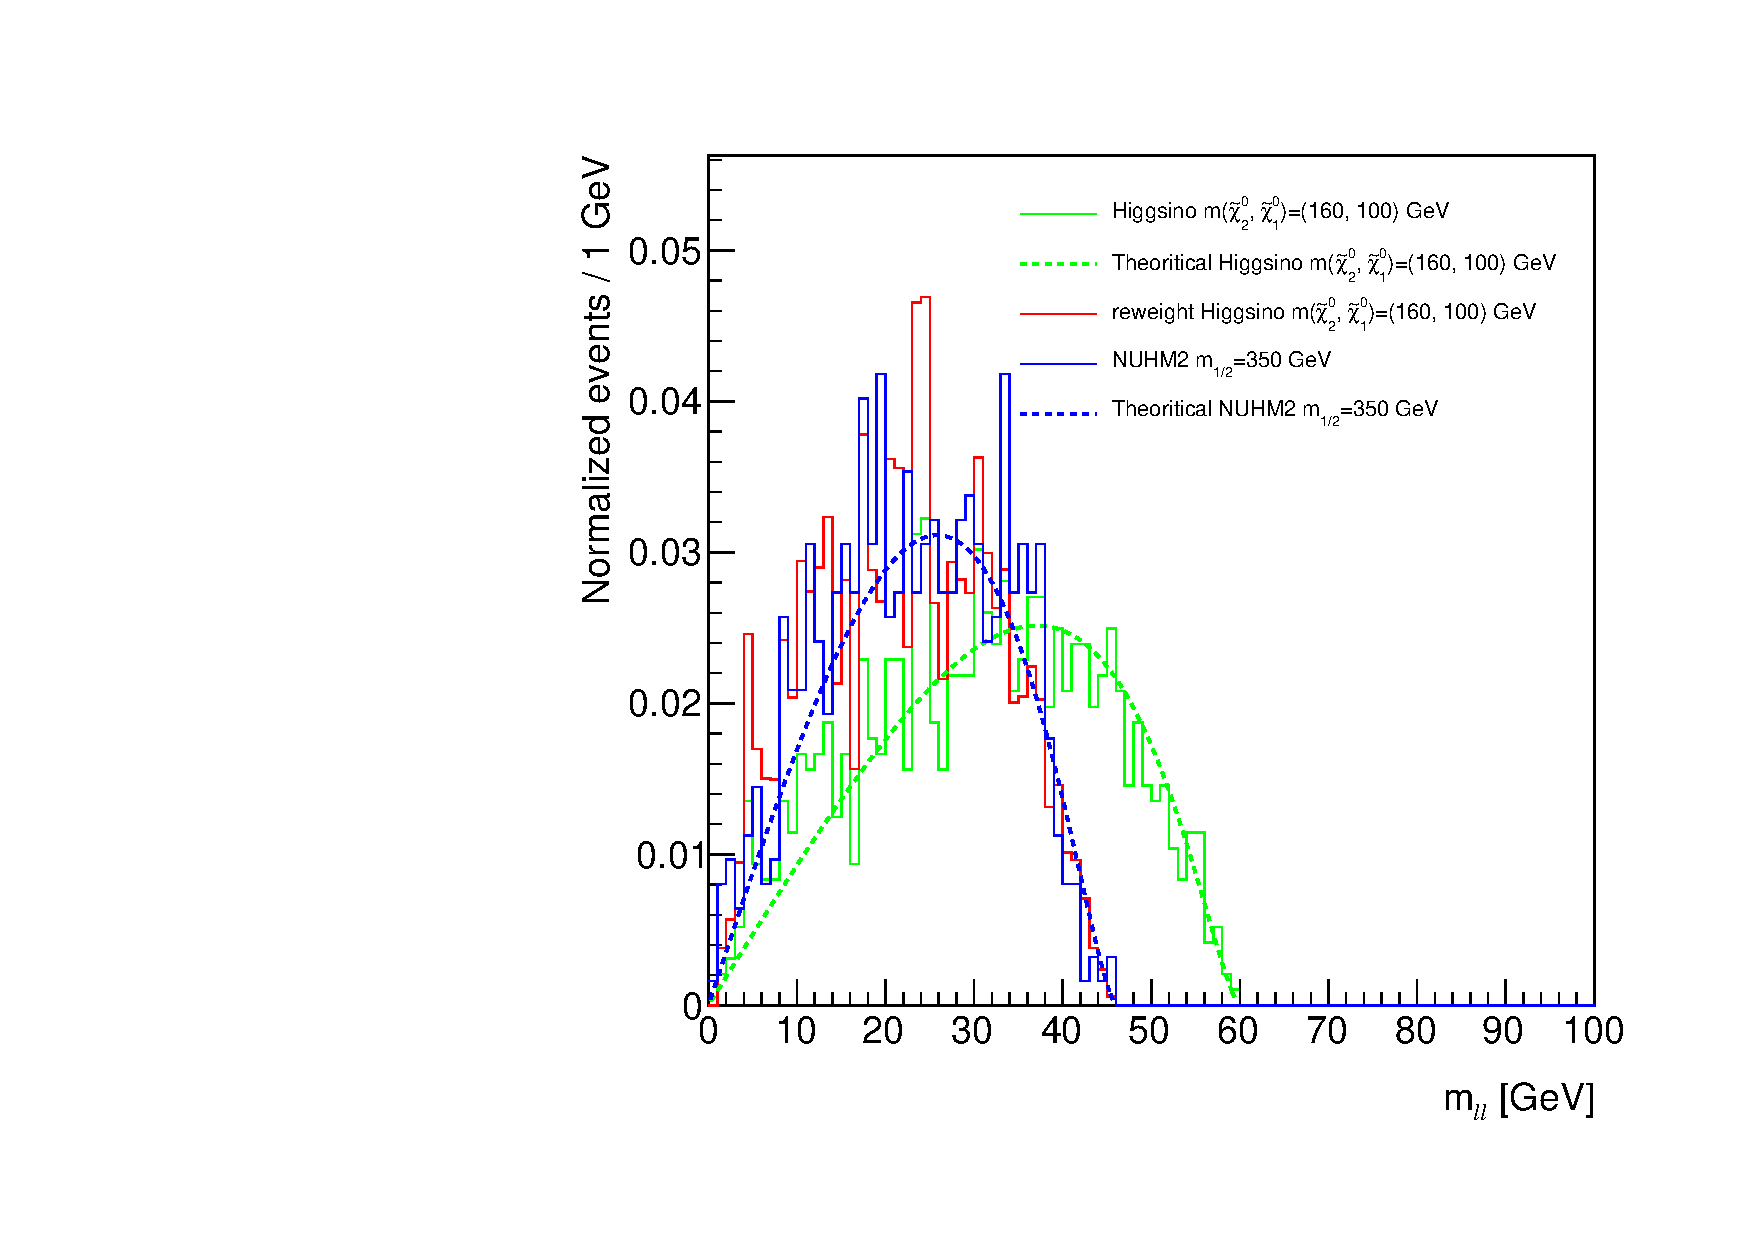
\includegraphics[scale=0.35]{reweight_Lorenzo_Higgsino_160_100_m12_350.pdf}
            \caption{NUHM2 $m_{1/2}=350$~{\GeV}}
        \end{subfigure}
        \begin{subfigure}[b]{0.48\textwidth}
            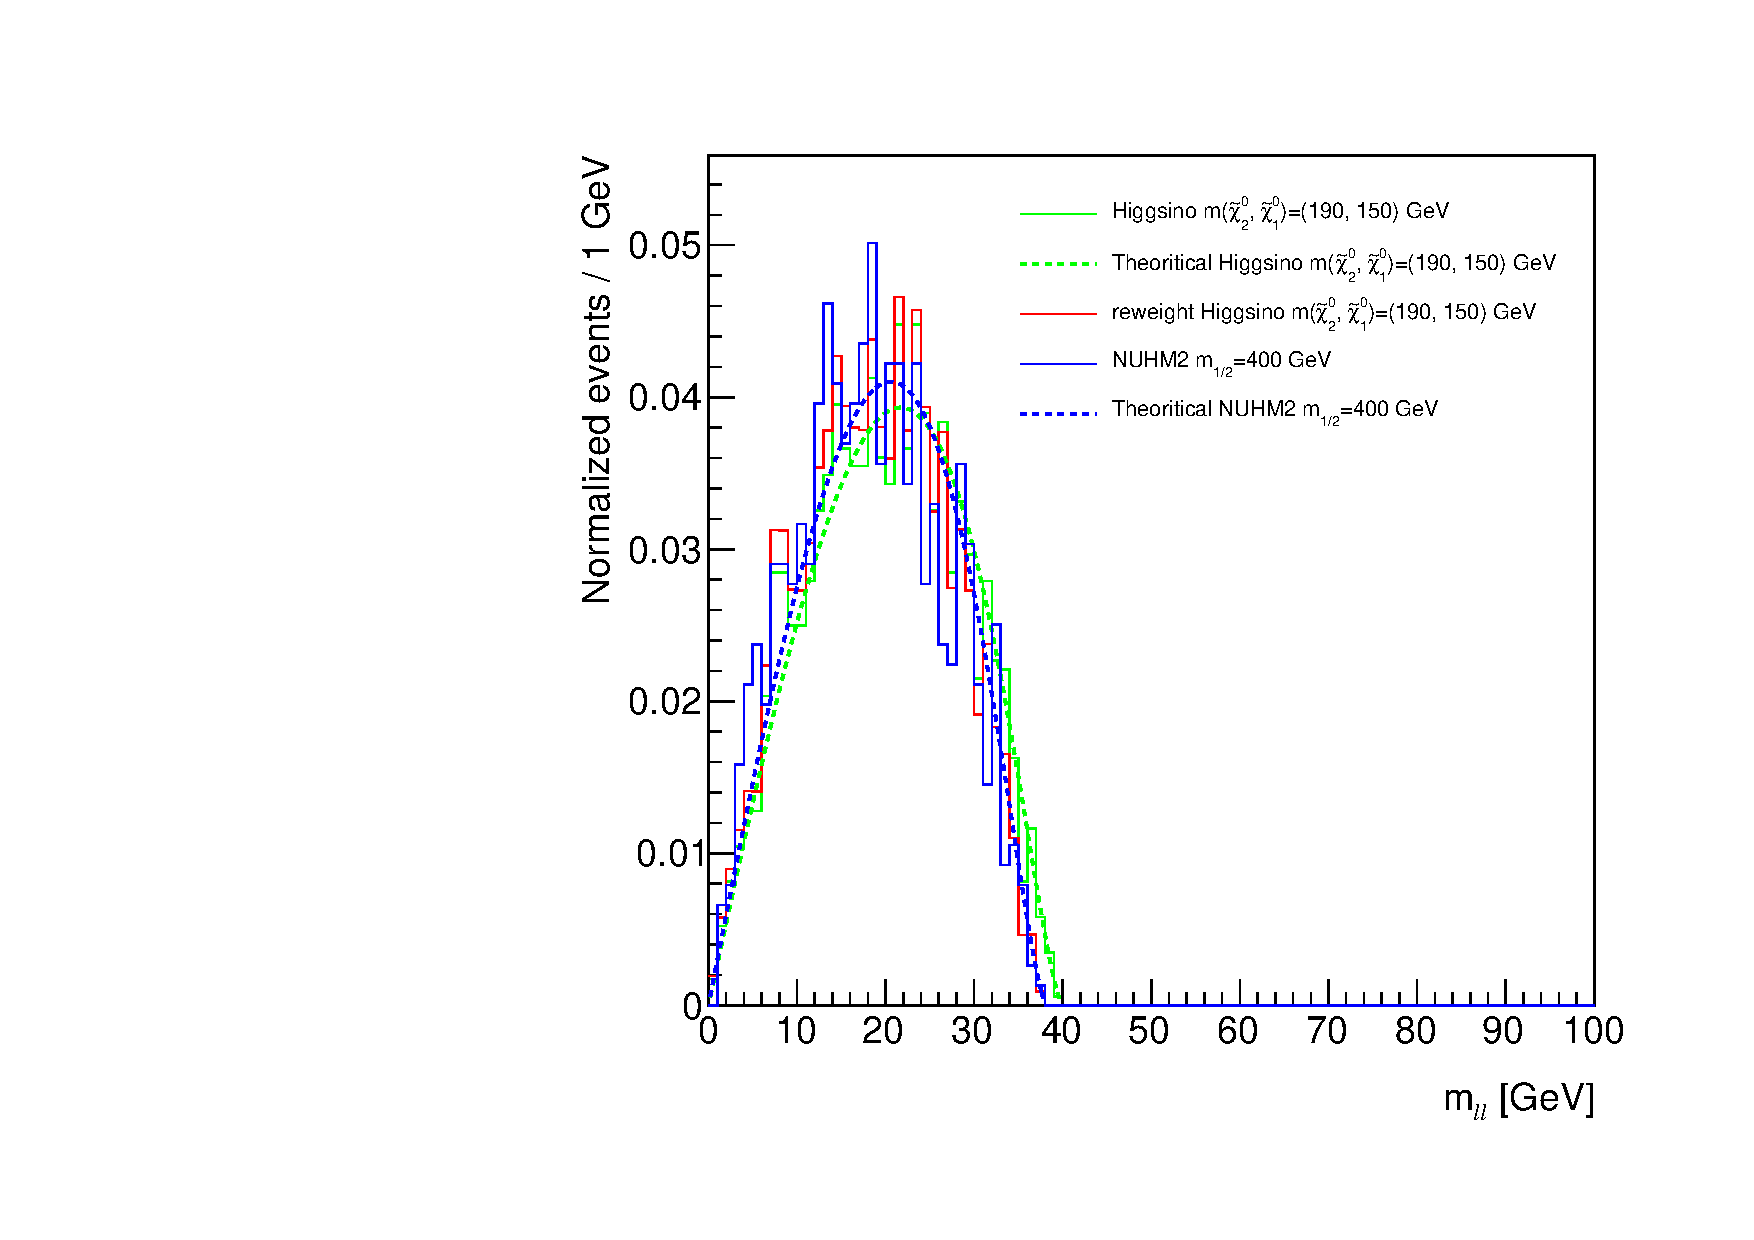
\includegraphics[scale=0.35]{reweight_Lorenzo_Higgsino_190_150_m12_400.pdf}
            \caption{NUHM2 $m_{1/2}=400$~{\GeV}}
        \end{subfigure}
        \begin{subfigure}[b]{0.48\textwidth}
            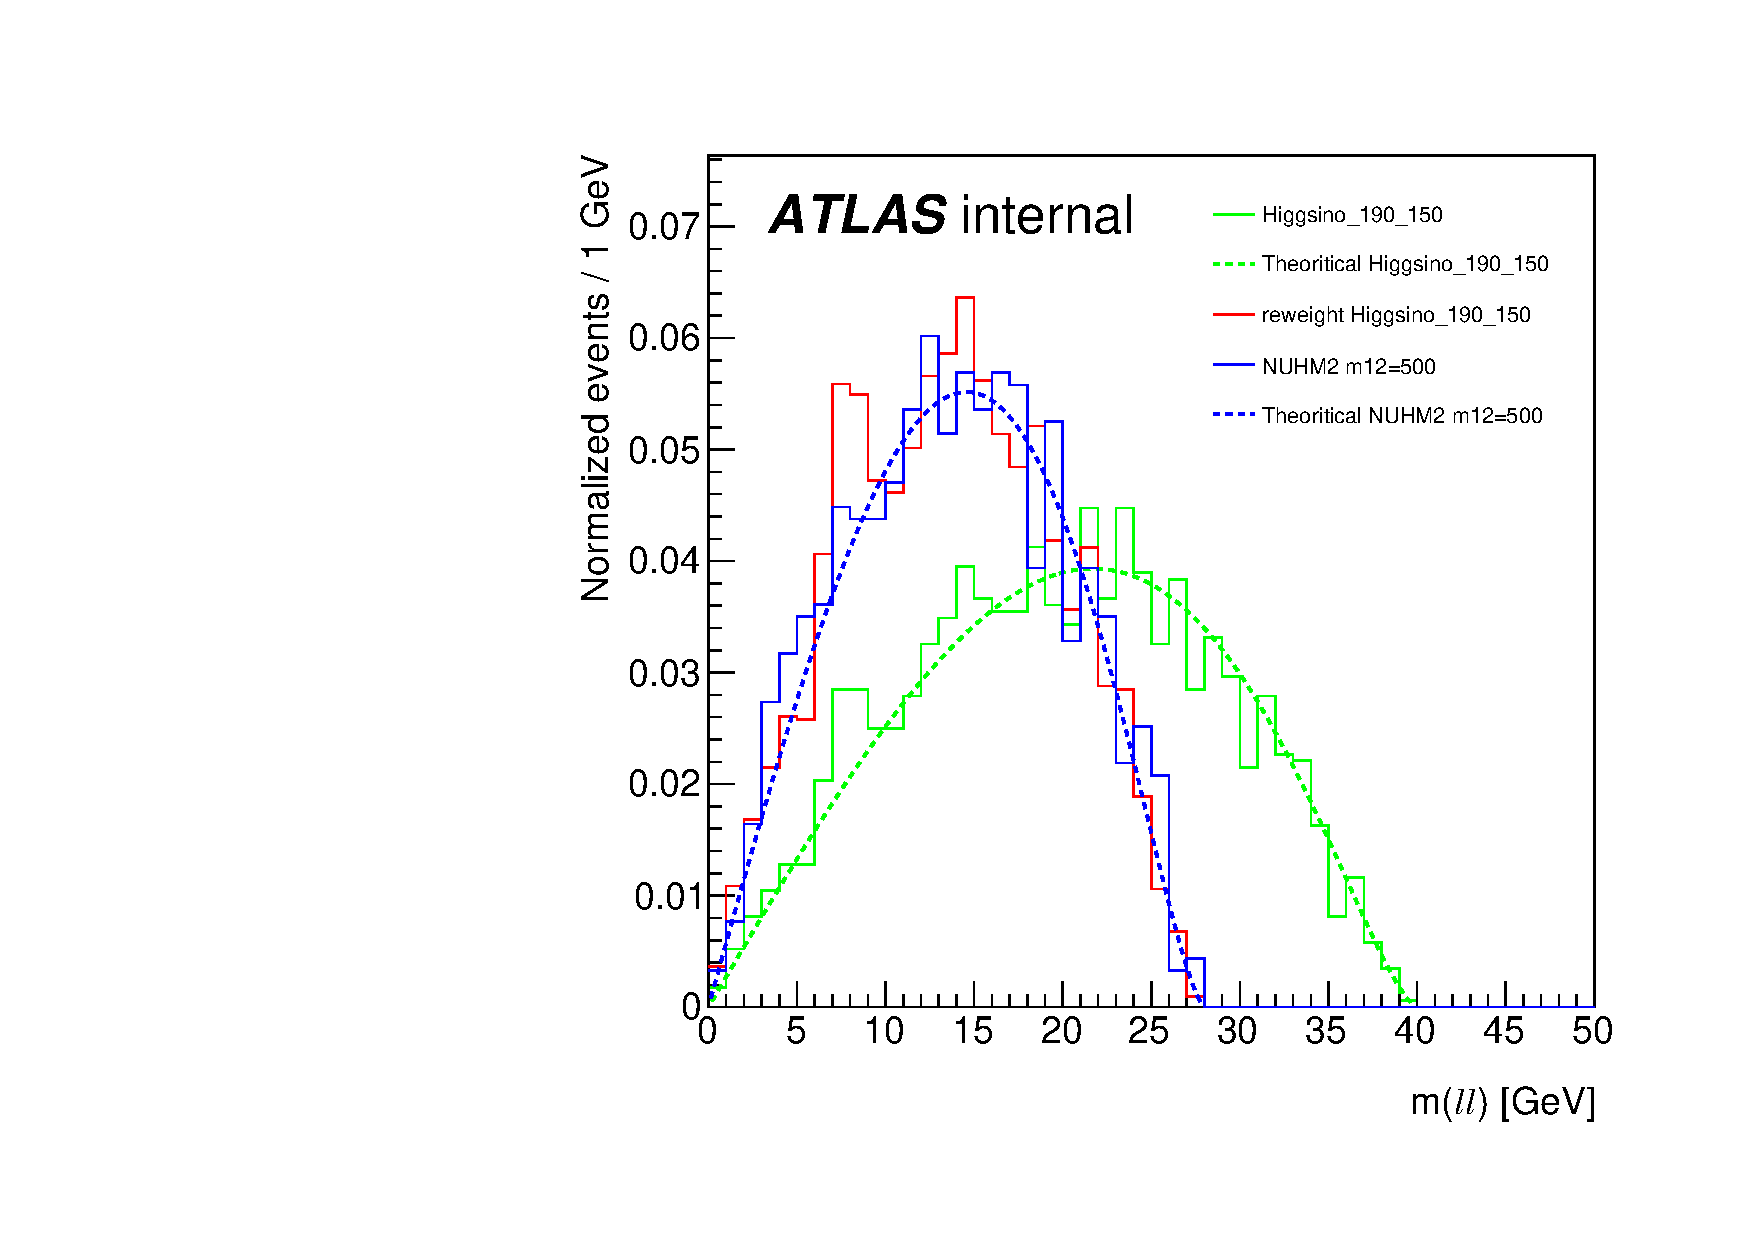
\includegraphics[scale=0.35]{reweight_Lorenzo_Higgsino_190_150_m12_500.pdf}
            \caption{NUHM2 $m_{1/2}=500$~{\GeV}}
        \end{subfigure}
        \begin{subfigure}[b]{0.48\textwidth}
            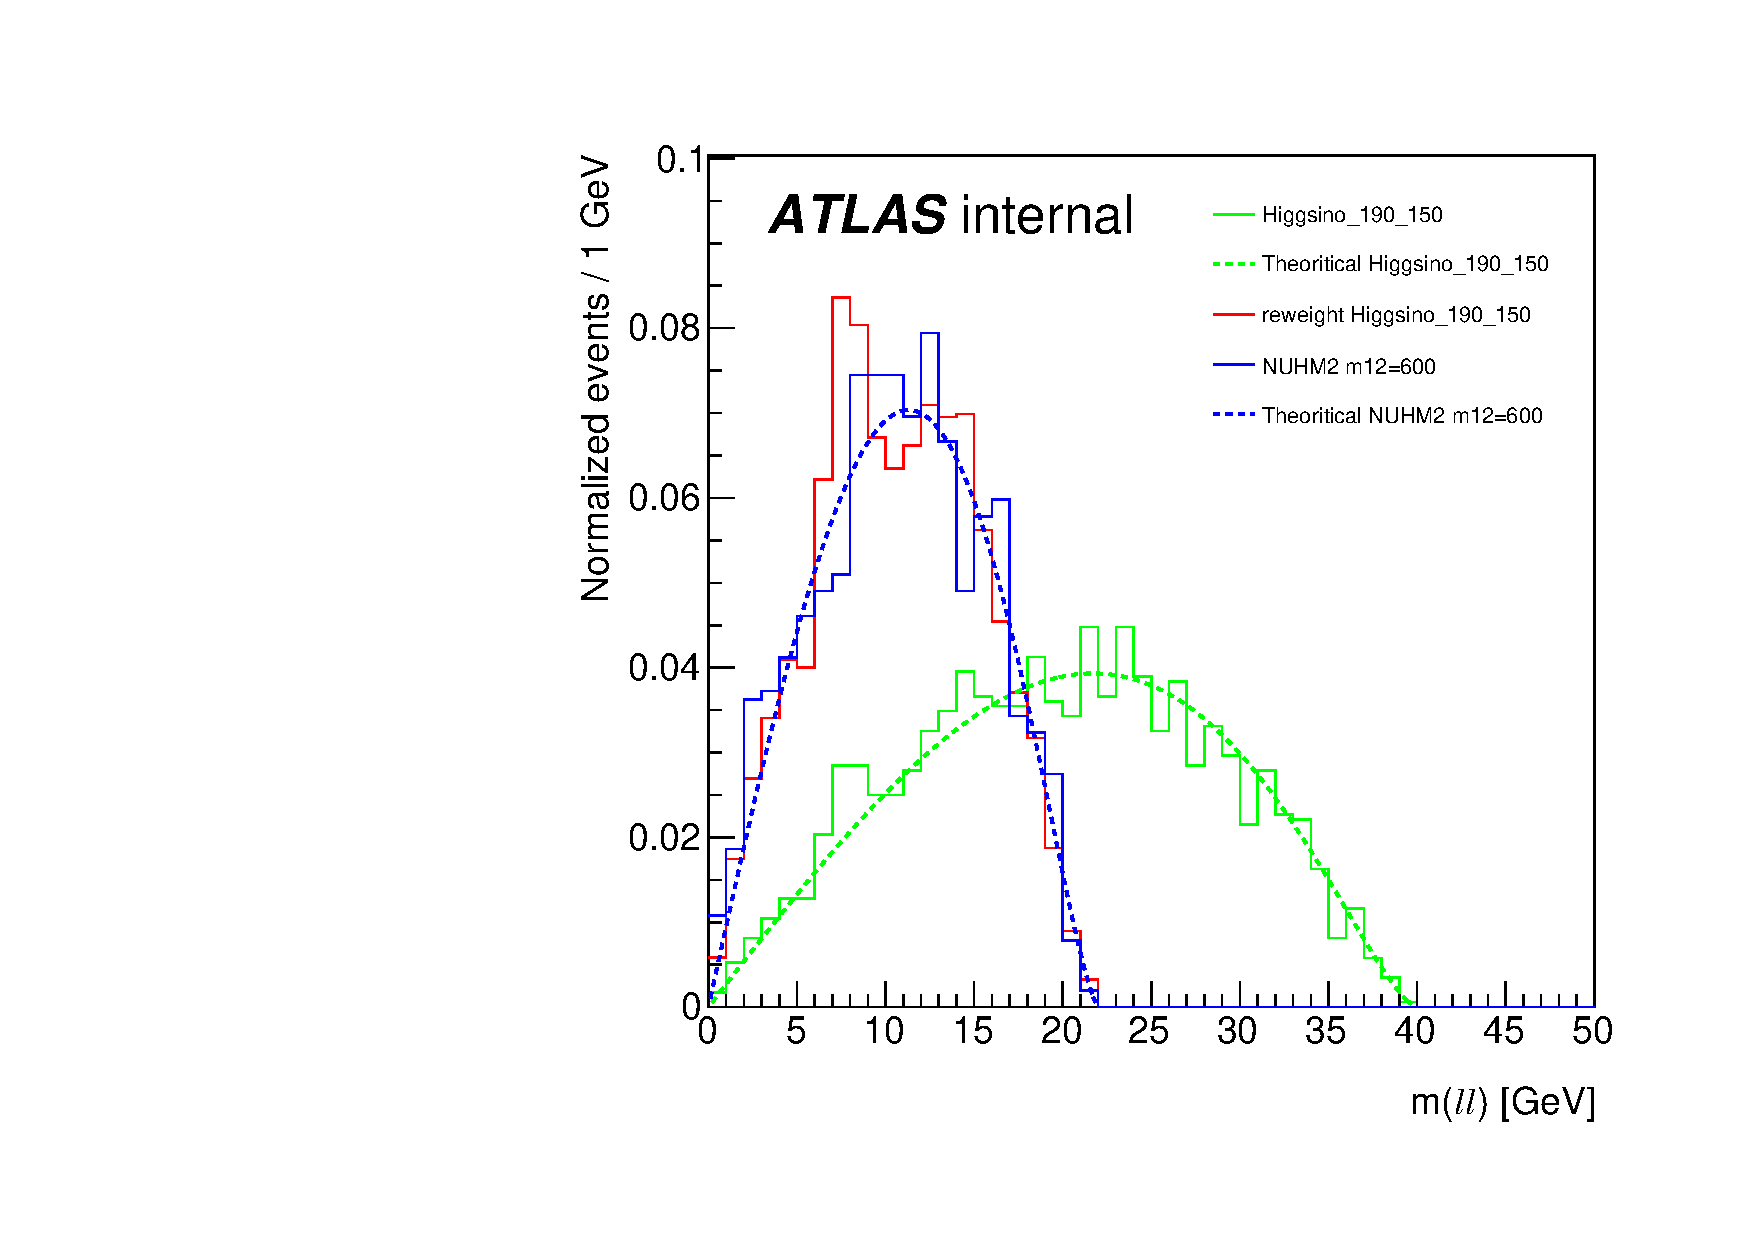
\includegraphics[scale=0.35]{reweight_Lorenzo_Higgsino_190_150_m12_600.pdf}
            \caption{NUHM2 $m_{1/2}=600$~{\GeV}}
        \end{subfigure}
        \begin{subfigure}[b]{0.48\textwidth}
            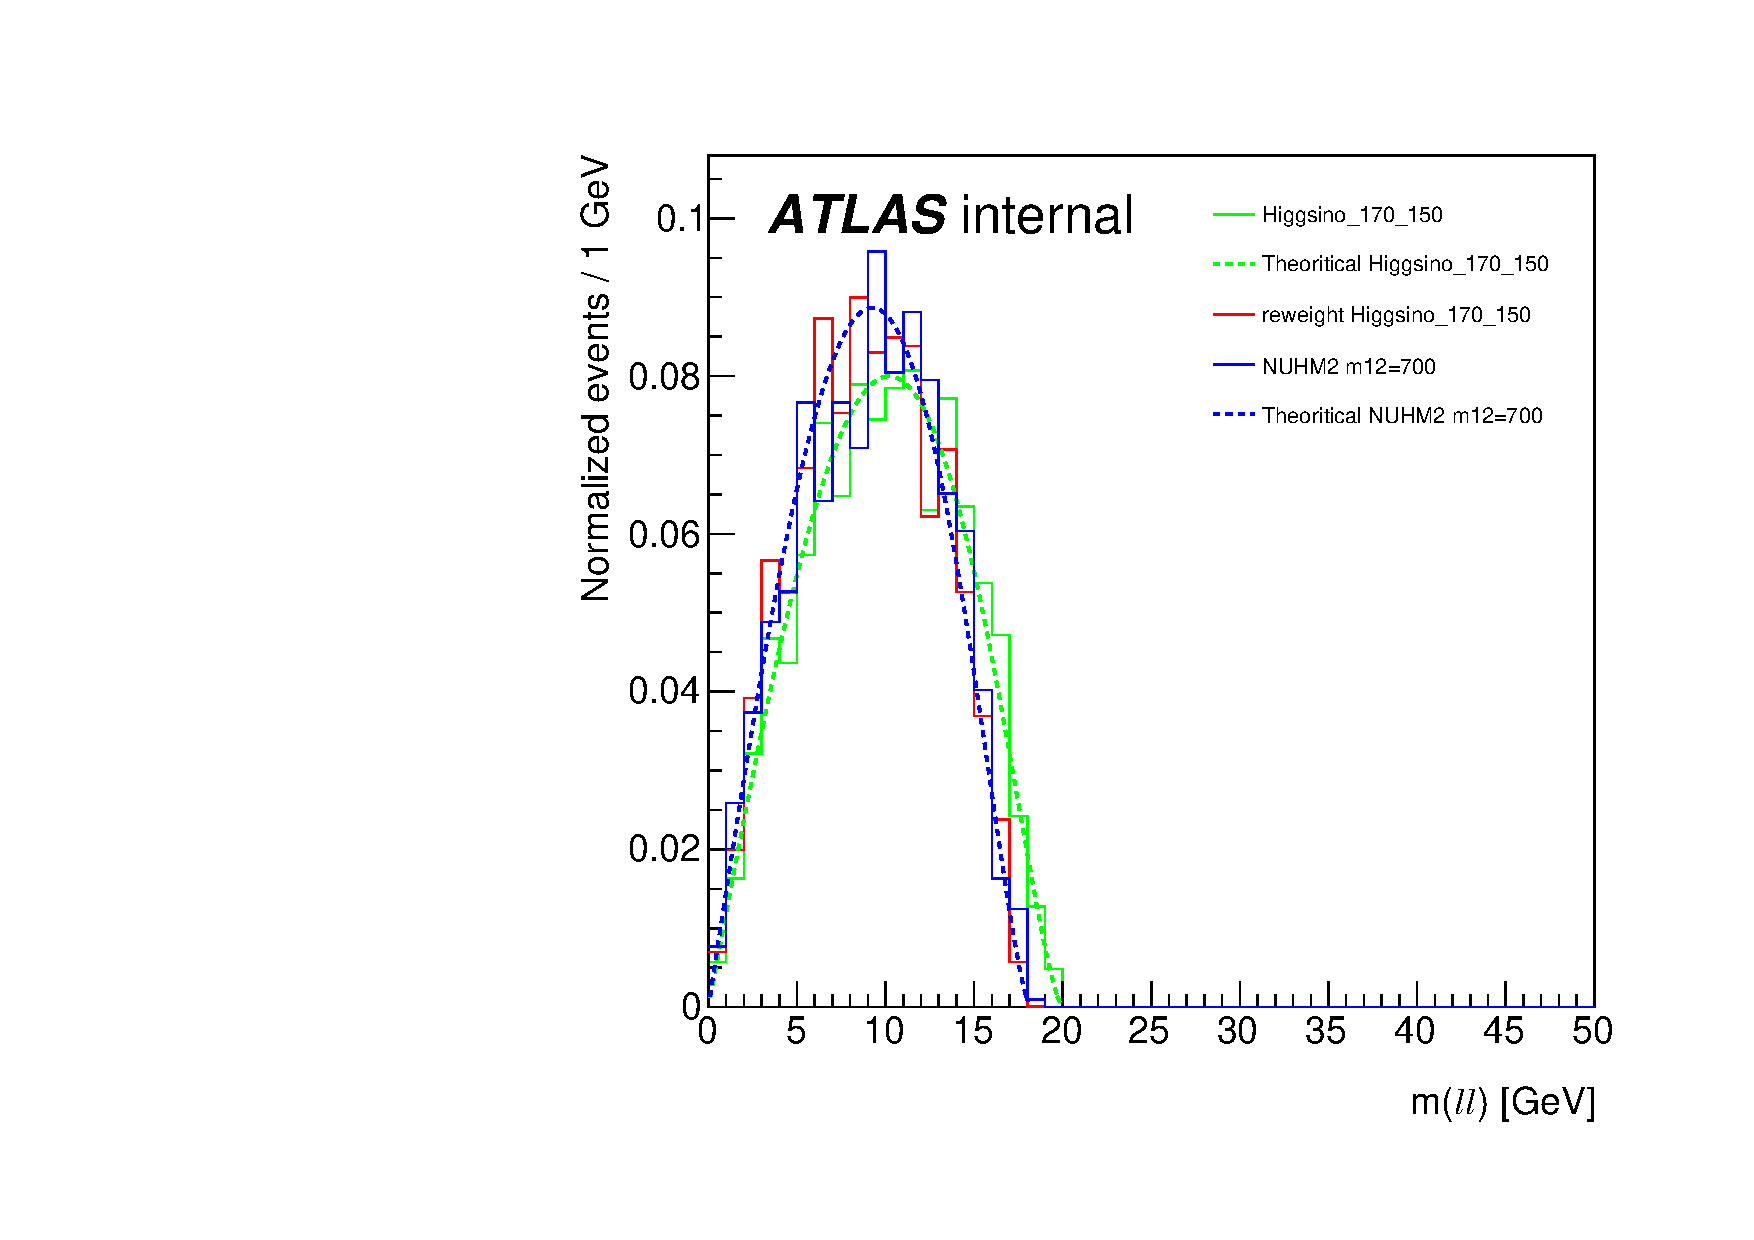
\includegraphics[scale=0.35]{reweight_Lorenzo_Higgsino_170_150_m12_700.pdf}
            \caption{NUHM2 $m_{1/2}=700$~{\GeV}}
        \end{subfigure}
        \begin{subfigure}[b]{0.48\textwidth}
            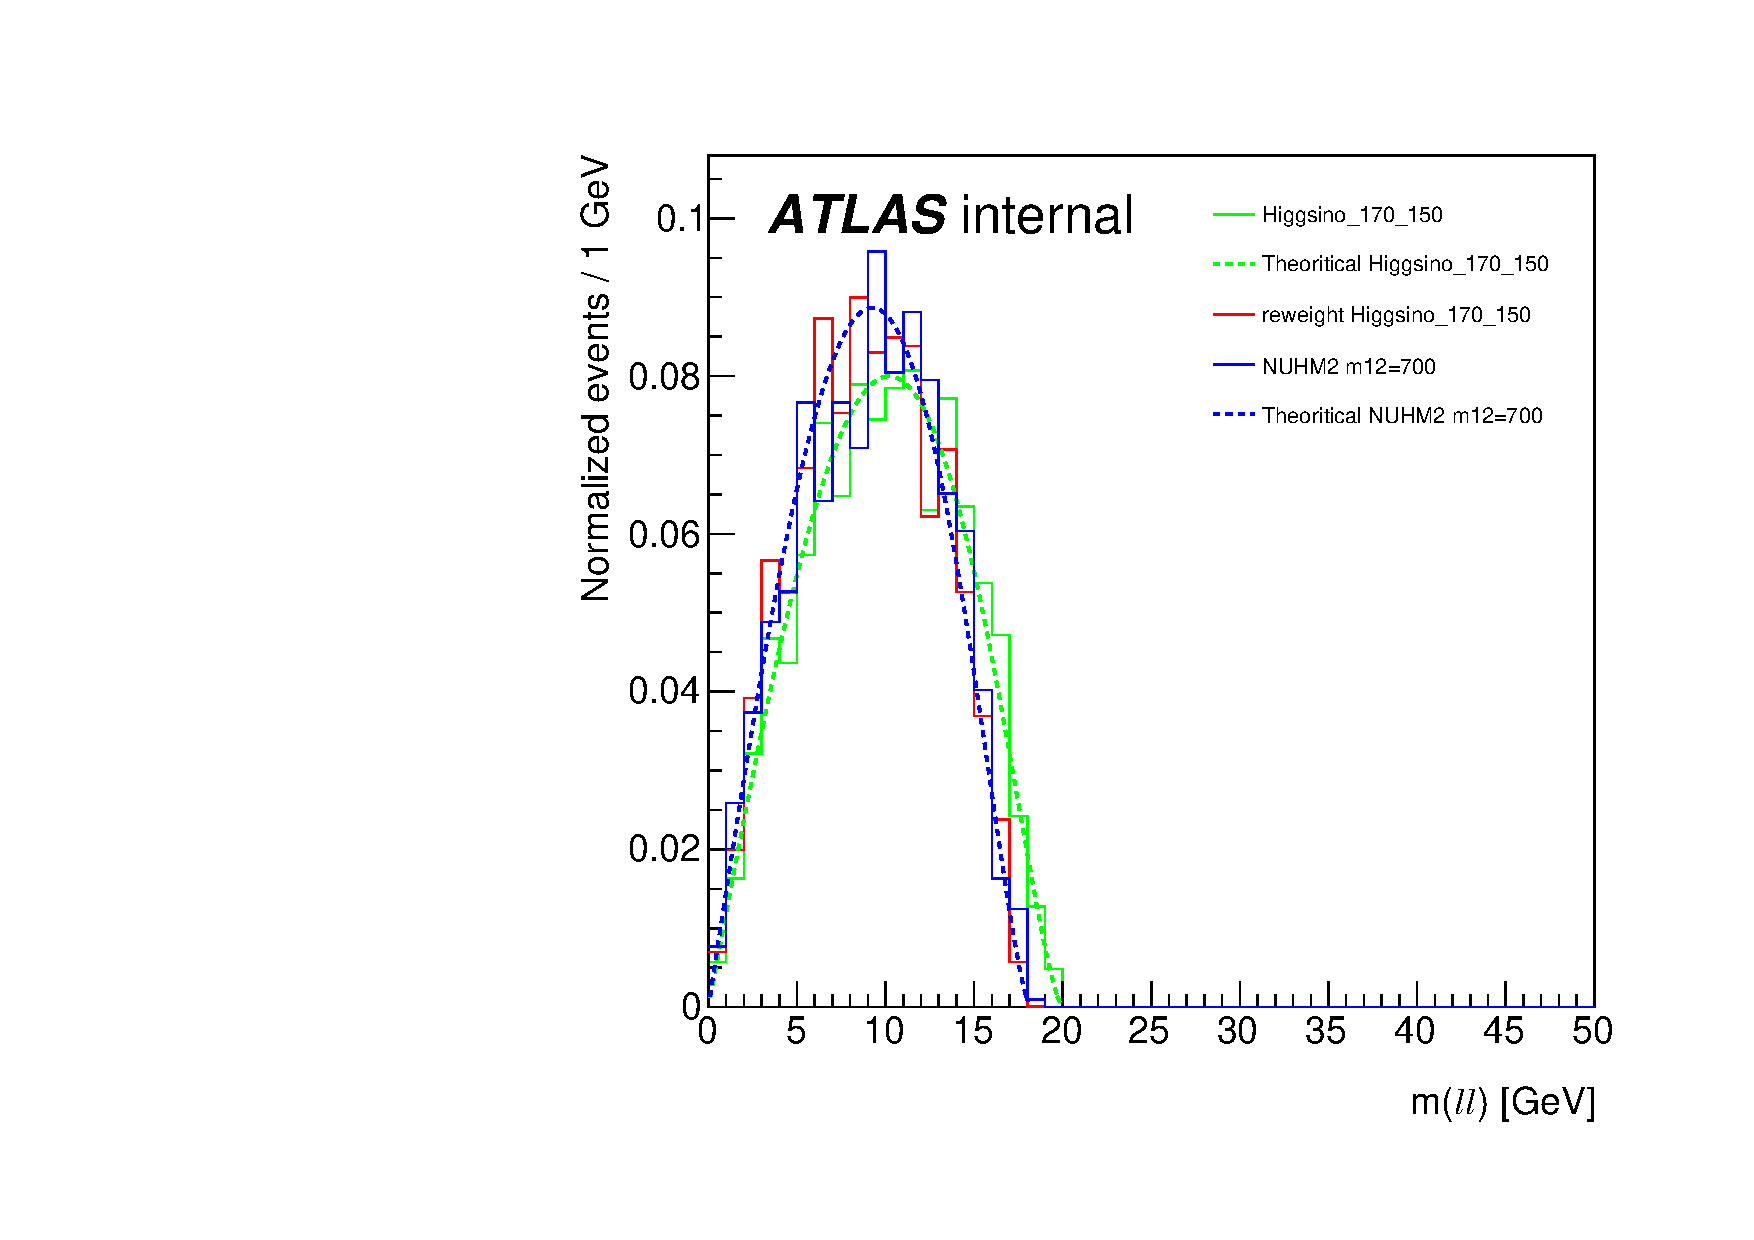
\includegraphics[scale=0.35]{reweight_Lorenzo_Higgsino_170_150_m12_700.pdf}
            \caption{NUHM2 $m_{1/2}=800$~{\GeV}}
        \end{subfigure}
    \end{center}
    % \caption{The $m_{\ell \ell}$ distributions for the NUHM2 and simplified Higgsino model.



    % \mll re-weighting method for the NUHM2 using Higgsino samples.
    % The blue solid line and green solid line are the truth $m_{\ell\ell}$ distributions for the NUHM2 and Higgsino, respectively.
    % The green dashed line is the \mll distribution obtained from the formula for the Higgsino sample.
    % The good agreement between green solid line and green dashed line indicates the robustness of the formula.
    % The event-by-event re-weighting of the Higgsino to the NUHM2 \mll distribution is shown in red solid line which matches the \mll distribution for the NUHM2 predicted by the formula (blue dashed line).
    % }
    \label{fig:results_nuhm2_reweighting}
\end{figure}




%%%
%%%
%%%

\section{NUHM2 interpretation using the MC production}
\label{sec:results_mc_production}